\documentclass[twoside]{book}

% Packages required by doxygen
\usepackage{fixltx2e}
\usepackage{calc}
\usepackage{doxygen}
\usepackage[export]{adjustbox} % also loads graphicx
\usepackage{graphicx}
\usepackage[utf8]{inputenc}
\usepackage{makeidx}
\usepackage{multicol}
\usepackage{multirow}
\PassOptionsToPackage{warn}{textcomp}
\usepackage{textcomp}
\usepackage[nointegrals]{wasysym}
\usepackage[table]{xcolor}

% Font selection
\usepackage[T1]{fontenc}
\usepackage[scaled=.90]{helvet}
\usepackage{courier}
\usepackage{amssymb}
\usepackage{sectsty}
\renewcommand{\familydefault}{\sfdefault}
\allsectionsfont{%
  \fontseries{bc}\selectfont%
  \color{darkgray}%
}
\renewcommand{\DoxyLabelFont}{%
  \fontseries{bc}\selectfont%
  \color{darkgray}%
}
\newcommand{\+}{\discretionary{\mbox{\scriptsize$\hookleftarrow$}}{}{}}

% Page & text layout
\usepackage{geometry}
\geometry{%
  a4paper,%
  top=2.5cm,%
  bottom=2.5cm,%
  left=2.5cm,%
  right=2.5cm%
}
\tolerance=750
\hfuzz=15pt
\hbadness=750
\setlength{\emergencystretch}{15pt}
\setlength{\parindent}{0cm}
\setlength{\parskip}{3ex plus 2ex minus 2ex}
\makeatletter
\renewcommand{\paragraph}{%
  \@startsection{paragraph}{4}{0ex}{-1.0ex}{1.0ex}{%
    \normalfont\normalsize\bfseries\SS@parafont%
  }%
}
\renewcommand{\subparagraph}{%
  \@startsection{subparagraph}{5}{0ex}{-1.0ex}{1.0ex}{%
    \normalfont\normalsize\bfseries\SS@subparafont%
  }%
}
\makeatother

% Headers & footers
\usepackage{fancyhdr}
\pagestyle{fancyplain}
\fancyhead[LE]{\fancyplain{}{\bfseries\thepage}}
\fancyhead[CE]{\fancyplain{}{}}
\fancyhead[RE]{\fancyplain{}{\bfseries\leftmark}}
\fancyhead[LO]{\fancyplain{}{\bfseries\rightmark}}
\fancyhead[CO]{\fancyplain{}{}}
\fancyhead[RO]{\fancyplain{}{\bfseries\thepage}}
\fancyfoot[LE]{\fancyplain{}{}}
\fancyfoot[CE]{\fancyplain{}{}}
\fancyfoot[RE]{\fancyplain{}{\bfseries\scriptsize Generated by Doxygen }}
\fancyfoot[LO]{\fancyplain{}{\bfseries\scriptsize Generated by Doxygen }}
\fancyfoot[CO]{\fancyplain{}{}}
\fancyfoot[RO]{\fancyplain{}{}}
\renewcommand{\footrulewidth}{0.4pt}
\renewcommand{\chaptermark}[1]{%
  \markboth{#1}{}%
}
\renewcommand{\sectionmark}[1]{%
  \markright{\thesection\ #1}%
}

% Indices & bibliography
\usepackage{natbib}
\usepackage[titles]{tocloft}
\setcounter{tocdepth}{3}
\setcounter{secnumdepth}{5}
\makeindex

% Packages requested by user
\usepackage{mathtools}
\usepackage{amsfonts}
\usepackage{amsmath}
\usepackage{amssymb}

% Hyperlinks (required, but should be loaded last)
\usepackage{ifpdf}
\ifpdf
  \usepackage[pdftex,pagebackref=true]{hyperref}
\else
  \usepackage[ps2pdf,pagebackref=true]{hyperref}
\fi
\hypersetup{%
  colorlinks=true,%
  linkcolor=blue,%
  citecolor=blue,%
  unicode%
}

% Custom commands
\newcommand{\clearemptydoublepage}{%
  \newpage{\pagestyle{empty}\cleardoublepage}%
}

\usepackage{caption}
\captionsetup{labelsep=space,justification=centering,font={bf},singlelinecheck=off,skip=4pt,position=top}

%===== C O N T E N T S =====

\begin{document}

% Titlepage & ToC
\hypersetup{pageanchor=false,
             bookmarksnumbered=true,
             pdfencoding=unicode
            }
\pagenumbering{alph}
\begin{titlepage}
\vspace*{7cm}
\begin{center}%
{\Large schwz \\[1ex]\large Generated automatically from event-\/test }\\
\vspace*{1cm}
{\large Generated by Doxygen 1.8.13}\\
\end{center}
\end{titlepage}
\clearemptydoublepage
\pagenumbering{roman}
\tableofcontents
\clearemptydoublepage
\pagenumbering{arabic}
\hypersetup{pageanchor=true}

%--- Begin generated contents ---
\chapter{Main Page}
\label{index}\hypertarget{index}{}This is the main page for the Schwarz library user documentation. The repository is hosted on \href{https://github.com/pratikvn/schwarz-lib}{\tt github}. Documentation on aspects such as the build system, can be found at the \hyperlink{install_schwarz}{\# Installation Instructions} page.

\subsubsection*{Modules}

The structure of the Schwarz Library code is divided into different \href{modules.html}{\tt modules} \+:


\begin{DoxyItemize}
\item \hyperlink{group__init}{Initialization} \+: Handles the initialization of the problem and the solver.
\item \hyperlink{group__comm}{Communicate} \+: Handles the communication.
\item \hyperlink{group__solve}{Solve} \+: Handles the local solution and the convergence detection.
\item \hyperlink{group__schwarz__class}{Schwarz Class} \+: The Classes related to the Schwarz solvers.
\item \hyperlink{group__utils}{Utils} \+: Provides some basic utilities. 
\end{DoxyItemize}
\chapter{\# Installation Instructions}
\label{install_schwarz}
\Hypertarget{install_schwarz}
\subsection*{Building}

Use the standard cmake build procedure\+:


\begin{DoxyCode}
mkdir build; cd build
cmake -G "Unix Makefiles" [OPTIONS] .. && make
\end{DoxyCode}


Replace {\ttfamily \mbox{[}O\+P\+T\+I\+O\+NS\mbox{]}} with desired cmake options for your build. The library adds the following additional switches to control what is being built\+:


\begin{DoxyItemize}
\item {\ttfamily -\/\+D\+S\+C\+H\+W\+A\+R\+Z\+\_\+\+B\+U\+I\+L\+D\+\_\+\+B\+E\+N\+C\+H\+M\+A\+R\+K\+I\+NG=\{ON, O\+FF\}} Builds some example benchmarks. Default is {\ttfamily ON}
\item {\ttfamily -\/\+D\+S\+C\+H\+W\+A\+R\+Z\+\_\+\+B\+U\+I\+L\+D\+\_\+\+M\+E\+T\+IS=\{ON, O\+FF\}} Builds with support for the {\ttfamily M\+E\+T\+IS} partitioner. User needs to provide the path to the installation of the {\ttfamily M\+E\+T\+IS} library in {\ttfamily M\+E\+T\+I\+S\+\_\+\+D\+IR}, preferably as an environment variable. Default is {\ttfamily O\+FF}
\item {\ttfamily -\/\+D\+S\+C\+H\+W\+A\+R\+Z\+\_\+\+B\+U\+I\+L\+D\+\_\+\+C\+H\+O\+L\+M\+OD=\{ON, O\+FF\}} Builds with support for the {\ttfamily C\+H\+O\+L\+M\+OD} module from the Suitesparse library. User needs to set an environment variable {\ttfamily C\+H\+O\+L\+M\+O\+D\+\_\+\+D\+IR} to the path containing the {\ttfamily C\+H\+O\+L\+M\+OD} installation. Default is {\ttfamily O\+FF}
\item {\ttfamily -\/\+D\+S\+C\+H\+W\+A\+R\+Z\+\_\+\+B\+U\+I\+L\+D\+\_\+\+C\+U\+DA=\{ON, O\+FF\}} Builds with C\+U\+DA support. Though Ginkgo provides most of the required C\+U\+DA support, we do need to link to C\+U\+DA for explicit setting of G\+PU affinities, some custom gather and scatter operations. Default is {\ttfamily O\+FF}.
\item {\ttfamily -\/\+D\+S\+C\+H\+W\+A\+R\+Z\+\_\+\+B\+U\+I\+L\+D\+\_\+\+C\+L\+A\+N\+G\+\_\+\+T\+I\+DY=\{ON, O\+FF\}} Builds with support for {\ttfamily clang-\/tidy} Default is {\ttfamily O\+FF}
\item {\ttfamily -\/\+D\+S\+C\+H\+W\+A\+R\+Z\+\_\+\+B\+U\+I\+L\+D\+\_\+\+D\+E\+A\+L\+II=\{ON, O\+FF\}} Builds with support for the finite element library {\ttfamily deal.\+ii} Default is {\ttfamily O\+FF}
\item {\ttfamily -\/\+D\+S\+C\+H\+W\+A\+R\+Z\+\_\+\+W\+I\+T\+H\+\_\+\+H\+W\+L\+OC=\{ON, O\+FF\}} Builds with support for the hardware locality library used for binding hardware. {\ttfamily hwloc} is distributed as a part of the Open-\/\+M\+PI project. Default is {\ttfamily ON}
\item {\ttfamily -\/\+D\+S\+C\+H\+W\+A\+R\+Z\+\_\+\+D\+E\+V\+E\+L\+\_\+\+T\+O\+O\+LS=\{ON, O\+FF\}} Builds with some developer tools support. Default is {\ttfamily ON}. In particular uses \href{https://github.com/ginkgo-project/git-cmake-format}{\tt {\ttfamily git-\/cmake-\/format}} to automatically format the source files with {\ttfamily clang-\/format}.
\end{DoxyItemize}

\subsection*{Tips}


\begin{DoxyItemize}
\item If you are having C\+U\+DA problems and you are not using C\+U\+DA, then feel free to switch the C\+U\+DA module off with {\ttfamily -\/\+D\+S\+C\+H\+W\+A\+R\+Z\+\_\+\+B\+U\+I\+L\+D\+\_\+\+C\+U\+DA=off}.
\item Installing C\+H\+O\+L\+M\+OD can be a bit annoying. T\+O\+DO add some details on fixing Suitesparse compilation.
\item When doing merge commits it is possible that make format does not work. You can run {\ttfamily cmake -\/\+D\+S\+C\+H\+W\+A\+R\+Z\+\_\+\+D\+E\+V\+E\+L\+\_\+\+T\+O\+O\+LS=O\+FF ..} to temporarily switch off the formatting. Please switch it on again when committing normally. 
\end{DoxyItemize}
\chapter{Testing Instructions}
\label{testing_schwarz}
\Hypertarget{testing_schwarz}
Will be updated soon. 
\chapter{Benchmarking.}
\label{benchmarking_schwarz}
\Hypertarget{benchmarking_schwarz}
\section*{\# Generic Benchmark settings. }

The flag {\ttfamily -\/\+D\+S\+C\+H\+W\+A\+R\+Z\+\_\+\+B\+U\+I\+L\+D\+\_\+\+B\+E\+N\+C\+H\+M\+A\+R\+K\+I\+NG} (default {\ttfamily ON}) enables the examples and benchmarking snippets.

If {\ttfamily schwarz-\/lib} has been built with {\ttfamily deal.\+ii}, then the {\ttfamily deal.\+ii} examples, {\ttfamily ex\+\_\+6} and {\ttfamily ex\+\_\+9} are also built, else only the {\ttfamily bench\+\_\+ras} example is built. The following command line options are available for this example. This is setup using {\ttfamily gflags}.

The executable is run in the following fashion\+:

```sh \mbox{[}M\+P\+I\+\_\+\+C\+O\+M\+M\+A\+ND\mbox{]} \mbox{[}M\+P\+I\+\_\+\+O\+P\+T\+I\+O\+NS\mbox{]} 
\chapter{Module Index}
\section{Modules}
Here is a list of all modules\+:\begin{DoxyCompactList}
\item \contentsline{section}{Communicate}{\pageref{group__comm}}{}
\item \contentsline{section}{Initialization}{\pageref{group__init}}{}
\item \contentsline{section}{Schwarz Class}{\pageref{group__schwarz__class}}{}
\item \contentsline{section}{Solve}{\pageref{group__solve}}{}
\item \contentsline{section}{Utils}{\pageref{group__utils}}{}
\end{DoxyCompactList}

\chapter{Namespace Index}
\section{Namespace List}
Here is a list of all documented namespaces with brief descriptions\+:\begin{DoxyCompactList}
\item\contentsline{section}{\hyperlink{namespaceProcessTopology}{Process\+Topology} \\*The \hyperlink{namespaceProcessTopology}{Process\+Topology} namespace }{\pageref{namespaceProcessTopology}}{}
\item\contentsline{section}{\hyperlink{namespaceschwz}{schwz} \\*The Schwarz wrappers namespace }{\pageref{namespaceschwz}}{}
\item\contentsline{section}{\hyperlink{namespaceschwz_1_1CommHelpers}{schwz\+::\+Comm\+Helpers} \\*The Comm\+Helper namespace }{\pageref{namespaceschwz_1_1CommHelpers}}{}
\item\contentsline{section}{\hyperlink{namespaceschwz_1_1conv__tools}{schwz\+::conv\+\_\+tools} \\*The \hyperlink{namespaceschwz_1_1conv__tools}{conv\+\_\+tools} namespace }{\pageref{namespaceschwz_1_1conv__tools}}{}
\item\contentsline{section}{\hyperlink{namespaceschwz_1_1PartitionTools}{schwz\+::\+Partition\+Tools} \\*The \hyperlink{namespaceschwz_1_1PartitionTools}{Partition\+Tools} namespace }{\pageref{namespaceschwz_1_1PartitionTools}}{}
\item\contentsline{section}{\hyperlink{namespaceschwz_1_1SolverTools}{schwz\+::\+Solver\+Tools} \\*The \hyperlink{namespaceschwz_1_1SolverTools}{Solver\+Tools} namespace }{\pageref{namespaceschwz_1_1SolverTools}}{}
\end{DoxyCompactList}

\chapter{Hierarchical Index}
\section{Class Hierarchy}
This inheritance list is sorted roughly, but not completely, alphabetically\+:\begin{DoxyCompactList}
\item \contentsline{section}{schwz\+:\+:Settings\+:\+:comm\+\_\+settings}{\pageref{structschwz_1_1Settings_1_1comm__settings}}{}
\item \contentsline{section}{schwz\+:\+:Communicate$<$ Value\+Type, Index\+Type, Mixed\+Value\+Type $>$\+:\+:comm\+\_\+struct}{\pageref{structschwz_1_1Communicate_1_1comm__struct}}{}
\item \contentsline{section}{schwz\+:\+:Communicate$<$ Value\+Type, Index\+Type, Mixed\+Value\+Type $>$}{\pageref{classschwz_1_1Communicate}}{}
\begin{DoxyCompactList}
\item \contentsline{section}{schwz\+:\+:Schwarz\+Base$<$ Value\+Type, Index\+Type, Mixed\+Value\+Type $>$}{\pageref{classschwz_1_1SchwarzBase}}{}
\begin{DoxyCompactList}
\item \contentsline{section}{schwz\+:\+:Solver\+R\+AS$<$ Value\+Type, Index\+Type, Mixed\+Value\+Type $>$}{\pageref{classschwz_1_1SolverRAS}}{}
\end{DoxyCompactList}
\end{DoxyCompactList}
\item \contentsline{section}{schwz\+:\+:Settings\+:\+:convergence\+\_\+settings}{\pageref{structschwz_1_1Settings_1_1convergence__settings}}{}
\item \contentsline{section}{schwz\+:\+:device\+\_\+guard}{\pageref{classschwz_1_1device__guard}}{}
\item std\+:\+:exception\begin{DoxyCompactList}
\item \contentsline{section}{Error}{\pageref{classError}}{}
\begin{DoxyCompactList}
\item \contentsline{section}{Bad\+Dimension}{\pageref{classBadDimension}}{}
\item \contentsline{section}{Cuda\+Error}{\pageref{classCudaError}}{}
\item \contentsline{section}{Cusparse\+Error}{\pageref{classCusparseError}}{}
\item \contentsline{section}{Metis\+Error}{\pageref{classMetisError}}{}
\item \contentsline{section}{Module\+Not\+Implemented}{\pageref{classModuleNotImplemented}}{}
\item \contentsline{section}{Not\+Implemented}{\pageref{classNotImplemented}}{}
\item \contentsline{section}{Umfpack\+Error}{\pageref{classUmfpackError}}{}
\end{DoxyCompactList}
\end{DoxyCompactList}
\item \contentsline{section}{schwz\+:\+:Metadata$<$ Value\+Type, Index\+Type $>$}{\pageref{structschwz_1_1Metadata}}{}
\begin{DoxyCompactList}
\item \contentsline{section}{schwz\+:\+:Initialize$<$ Value\+Type, Index\+Type $>$}{\pageref{classschwz_1_1Initialize}}{}
\begin{DoxyCompactList}
\item \contentsline{section}{schwz\+:\+:Schwarz\+Base$<$ Value\+Type, Index\+Type, Mixed\+Value\+Type $>$}{\pageref{classschwz_1_1SchwarzBase}}{}
\end{DoxyCompactList}
\end{DoxyCompactList}
\item Operation\begin{DoxyCompactList}
\item \contentsline{section}{schwz\+:\+:Gather$<$ Value\+Type, Index\+Type $>$}{\pageref{structschwz_1_1Gather}}{}
\item \contentsline{section}{schwz\+:\+:Scatter$<$ Value\+Type, Index\+Type $>$}{\pageref{structschwz_1_1Scatter}}{}
\end{DoxyCompactList}
\item \contentsline{section}{schwz\+:\+:Metadata$<$ Value\+Type, Index\+Type $>$\+:\+:post\+\_\+process\+\_\+data}{\pageref{structschwz_1_1Metadata_1_1post__process__data}}{}
\item \contentsline{section}{schwz\+:\+:Settings}{\pageref{structschwz_1_1Settings}}{}
\begin{DoxyCompactList}
\item \contentsline{section}{schwz\+:\+:Initialize$<$ Value\+Type, Index\+Type $>$}{\pageref{classschwz_1_1Initialize}}{}
\item \contentsline{section}{schwz\+:\+:Solve$<$ Value\+Type, Index\+Type, Mixed\+Value\+Type $>$}{\pageref{classschwz_1_1Solve}}{}
\begin{DoxyCompactList}
\item \contentsline{section}{schwz\+:\+:Schwarz\+Base$<$ Value\+Type, Index\+Type, Mixed\+Value\+Type $>$}{\pageref{classschwz_1_1SchwarzBase}}{}
\end{DoxyCompactList}
\end{DoxyCompactList}
\item \contentsline{section}{schwz\+:\+:Utils$<$ Value\+Type, Index\+Type $>$}{\pageref{structschwz_1_1Utils}}{}
\end{DoxyCompactList}

\chapter{Class Index}
\section{Class List}
Here are the classes, structs, unions and interfaces with brief descriptions\+:\begin{DoxyCompactList}
\item\contentsline{section}{\hyperlink{classBadDimension}{Bad\+Dimension} \\*\hyperlink{classBadDimension}{Bad\+Dimension} is thrown if an operation is being applied to a Lin\+Op with bad dimensions }{\pageref{classBadDimension}}{}
\item\contentsline{section}{\hyperlink{structschwz_1_1Settings_1_1comm__settings}{schwz\+::\+Settings\+::comm\+\_\+settings} \\*The settings for the various available communication paradigms }{\pageref{structschwz_1_1Settings_1_1comm__settings}}{}
\item\contentsline{section}{\hyperlink{structschwz_1_1Communicate_1_1comm__struct}{schwz\+::\+Communicate$<$ Value\+Type, Index\+Type, Mixed\+Value\+Type $>$\+::comm\+\_\+struct} \\*The communication struct used to store the communication data }{\pageref{structschwz_1_1Communicate_1_1comm__struct}}{}
\item\contentsline{section}{\hyperlink{classschwz_1_1Communicate}{schwz\+::\+Communicate$<$ Value\+Type, Index\+Type, Mixed\+Value\+Type $>$} \\*The communication class that provides the methods for the communication between the subdomains }{\pageref{classschwz_1_1Communicate}}{}
\item\contentsline{section}{\hyperlink{structschwz_1_1Settings_1_1convergence__settings}{schwz\+::\+Settings\+::convergence\+\_\+settings} \\*The various convergence settings available }{\pageref{structschwz_1_1Settings_1_1convergence__settings}}{}
\item\contentsline{section}{\hyperlink{classCudaError}{Cuda\+Error} \\*\hyperlink{classCudaError}{Cuda\+Error} is thrown when a C\+U\+DA routine throws a non-\/zero error code }{\pageref{classCudaError}}{}
\item\contentsline{section}{\hyperlink{classCusparseError}{Cusparse\+Error} \\*\hyperlink{classCusparseError}{Cusparse\+Error} is thrown when a cu\+S\+P\+A\+R\+SE routine throws a non-\/zero error code }{\pageref{classCusparseError}}{}
\item\contentsline{section}{\hyperlink{classschwz_1_1device__guard}{schwz\+::device\+\_\+guard} \\*This class defines a device guard for the cuda functions and the cuda module }{\pageref{classschwz_1_1device__guard}}{}
\item\contentsline{section}{\hyperlink{classError}{Error} }{\pageref{classError}}{}
\item\contentsline{section}{\hyperlink{structGatherScatter}{Gather\+Scatter$<$ Value\+Type, Index\+Type $>$} }{\pageref{structGatherScatter}}{}
\item\contentsline{section}{\hyperlink{classschwz_1_1Initialize}{schwz\+::\+Initialize$<$ Value\+Type, Index\+Type $>$} \\*The initialization class that provides methods for initialization of the solver }{\pageref{classschwz_1_1Initialize}}{}
\item\contentsline{section}{\hyperlink{structschwz_1_1Metadata}{schwz\+::\+Metadata$<$ Value\+Type, Index\+Type $>$} \\*The solver metadata struct }{\pageref{structschwz_1_1Metadata}}{}
\item\contentsline{section}{\hyperlink{classMetisError}{Metis\+Error} \\*\hyperlink{classMetisError}{Metis\+Error} is thrown when a M\+E\+T\+IS routine throws a non-\/zero error code }{\pageref{classMetisError}}{}
\item\contentsline{section}{\hyperlink{classModuleNotImplemented}{Module\+Not\+Implemented} }{\pageref{classModuleNotImplemented}}{}
\item\contentsline{section}{\hyperlink{classNotImplemented}{Not\+Implemented} }{\pageref{classNotImplemented}}{}
\item\contentsline{section}{\hyperlink{structschwz_1_1Metadata_1_1post__process__data}{schwz\+::\+Metadata$<$ Value\+Type, Index\+Type $>$\+::post\+\_\+process\+\_\+data} \\*The struct used for storing data for post-\/processing }{\pageref{structschwz_1_1Metadata_1_1post__process__data}}{}
\item\contentsline{section}{\hyperlink{classschwz_1_1SchwarzBase}{schwz\+::\+Schwarz\+Base$<$ Value\+Type, Index\+Type, Mixed\+Value\+Type $>$} \\*The Base solver class is meant to be the class implementing the common implementations for all the schwarz methods }{\pageref{classschwz_1_1SchwarzBase}}{}
\item\contentsline{section}{\hyperlink{structschwz_1_1Settings}{schwz\+::\+Settings} \\*The struct that contains the solver settings and the parameters to be set by the user }{\pageref{structschwz_1_1Settings}}{}
\item\contentsline{section}{\hyperlink{classschwz_1_1Solve}{schwz\+::\+Solve$<$ Value\+Type, Index\+Type, Mixed\+Value\+Type $>$} \\*The Solver class the provides the solver and the convergence checking methods }{\pageref{classschwz_1_1Solve}}{}
\item\contentsline{section}{\hyperlink{classschwz_1_1SolverRAS}{schwz\+::\+Solver\+R\+A\+S$<$ Value\+Type, Index\+Type, Mixed\+Value\+Type $>$} \\*An implementation of the solver interface using the R\+AS solver }{\pageref{classschwz_1_1SolverRAS}}{}
\item\contentsline{section}{\hyperlink{classUmfpackError}{Umfpack\+Error} \\*\hyperlink{classUmfpackError}{Umfpack\+Error} is thrown when a M\+E\+T\+IS routine throws a non-\/zero error code }{\pageref{classUmfpackError}}{}
\item\contentsline{section}{\hyperlink{structschwz_1_1Utils}{schwz\+::\+Utils$<$ Value\+Type, Index\+Type $>$} \\*The utilities class which provides some checks and basic utilities }{\pageref{structschwz_1_1Utils}}{}
\end{DoxyCompactList}

\chapter{Module Documentation}
\hypertarget{group__comm}{}\section{Communicate}
\label{group__comm}\index{Communicate@{Communicate}}


A module dedicated to the Communication interface in schwarz-\/lib.  


Collaboration diagram for Communicate\+:
\nopagebreak
\begin{figure}[H]
\begin{center}
\leavevmode
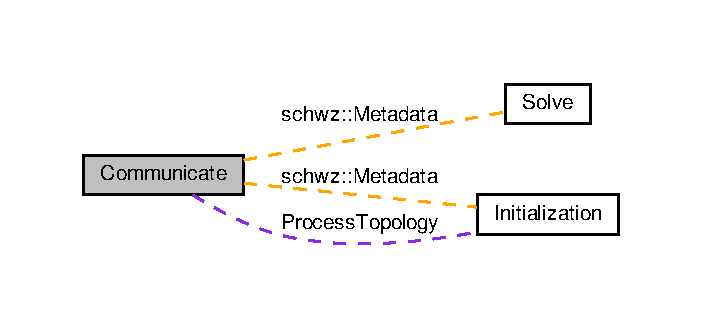
\includegraphics[width=350pt]{group__comm}
\end{center}
\end{figure}
\subsection*{Namespaces}
\begin{DoxyCompactItemize}
\item 
 \hyperlink{namespaceSchwarzWrappers_1_1CommHelpers}{Schwarz\+Wrappers\+::\+Comm\+Helpers}
\begin{DoxyCompactList}\small\item\em The Comm\+Helper namespace . \end{DoxyCompactList}\item 
 \hyperlink{namespaceProcessTopology}{Process\+Topology}
\begin{DoxyCompactList}\small\item\em The \hyperlink{namespaceProcessTopology}{Process\+Topology} namespace . \end{DoxyCompactList}\end{DoxyCompactItemize}
\subsection*{Classes}
\begin{DoxyCompactItemize}
\item 
class \hyperlink{classSchwarzWrappers_1_1Communicate}{Schwarz\+Wrappers\+::\+Communicate$<$ Value\+Type, Index\+Type $>$}
\begin{DoxyCompactList}\small\item\em The communication class that provides the methods for the communication between the subdomains. \end{DoxyCompactList}\item 
struct \hyperlink{structSchwarzWrappers_1_1Metadata}{Schwarz\+Wrappers\+::\+Metadata$<$ Value\+Type, Index\+Type $>$}
\begin{DoxyCompactList}\small\item\em The solver metadata struct. \end{DoxyCompactList}\end{DoxyCompactItemize}


\subsection{Detailed Description}
A module dedicated to the Communication interface in schwarz-\/lib. 


\hypertarget{group__init}{}\section{Initialization}
\label{group__init}\index{Initialization@{Initialization}}


A module dedicated to the initialization and setup and usage of the solvers in schwarz-\/lib.  


Collaboration diagram for Initialization\+:
\nopagebreak
\begin{figure}[H]
\begin{center}
\leavevmode
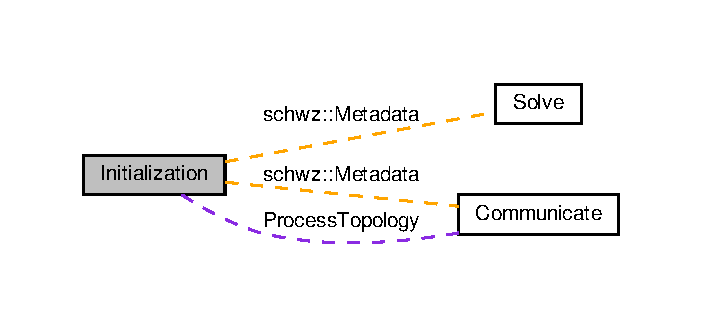
\includegraphics[width=350pt]{group__init}
\end{center}
\end{figure}
\subsection*{Namespaces}
\begin{DoxyCompactItemize}
\item 
 \hyperlink{namespaceSchwarzWrappers_1_1PartitionTools}{Schwarz\+Wrappers\+::\+Partition\+Tools}
\begin{DoxyCompactList}\small\item\em The \hyperlink{namespaceSchwarzWrappers_1_1PartitionTools}{Partition\+Tools} namespace . \end{DoxyCompactList}\item 
 \hyperlink{namespaceProcessTopology}{Process\+Topology}
\begin{DoxyCompactList}\small\item\em The \hyperlink{namespaceProcessTopology}{Process\+Topology} namespace . \end{DoxyCompactList}\end{DoxyCompactItemize}
\subsection*{Classes}
\begin{DoxyCompactItemize}
\item 
class \hyperlink{classSchwarzWrappers_1_1device__guard}{Schwarz\+Wrappers\+::device\+\_\+guard}
\begin{DoxyCompactList}\small\item\em This class defines a device guard for the cuda functions and the cuda module. \end{DoxyCompactList}\item 
class \hyperlink{classSchwarzWrappers_1_1Initialize}{Schwarz\+Wrappers\+::\+Initialize$<$ Value\+Type, Index\+Type $>$}
\begin{DoxyCompactList}\small\item\em The initialization class that provides methods for initialization of the solver. \end{DoxyCompactList}\item 
struct \hyperlink{structSchwarzWrappers_1_1Settings}{Schwarz\+Wrappers\+::\+Settings}
\begin{DoxyCompactList}\small\item\em The struct that contains the solver settings and the parameters to be set by the user. \end{DoxyCompactList}\item 
struct \hyperlink{structSchwarzWrappers_1_1Metadata}{Schwarz\+Wrappers\+::\+Metadata$<$ Value\+Type, Index\+Type $>$}
\begin{DoxyCompactList}\small\item\em The solver metadata struct. \end{DoxyCompactList}\end{DoxyCompactItemize}


\subsection{Detailed Description}
A module dedicated to the initialization and setup and usage of the solvers in schwarz-\/lib. 


\hypertarget{group__schwarz__class}{}\section{Schwarz Class}
\label{group__schwarz__class}\index{Schwarz Class@{Schwarz Class}}


A module dedicated to the Schwarz solver classes in schwarz-\/lib.  


\subsection*{Classes}
\begin{DoxyCompactItemize}
\item 
class \hyperlink{classschwz_1_1SolverRAS}{schwz\+::\+Solver\+R\+A\+S$<$ Value\+Type, Index\+Type, Mixed\+Value\+Type $>$}
\begin{DoxyCompactList}\small\item\em An implementation of the solver interface using the R\+AS solver. \end{DoxyCompactList}\item 
class \hyperlink{classschwz_1_1SchwarzBase}{schwz\+::\+Schwarz\+Base$<$ Value\+Type, Index\+Type, Mixed\+Value\+Type $>$}
\begin{DoxyCompactList}\small\item\em The Base solver class is meant to be the class implementing the common implementations for all the schwarz methods. \end{DoxyCompactList}\end{DoxyCompactItemize}


\subsection{Detailed Description}
A module dedicated to the Schwarz solver classes in schwarz-\/lib. 


\hypertarget{group__solve}{}\section{Solve}
\label{group__solve}\index{Solve@{Solve}}


A module dedicated to the solvers including local solution and convergence detection in schwarz-\/lib.  


Collaboration diagram for Solve\+:
\nopagebreak
\begin{figure}[H]
\begin{center}
\leavevmode
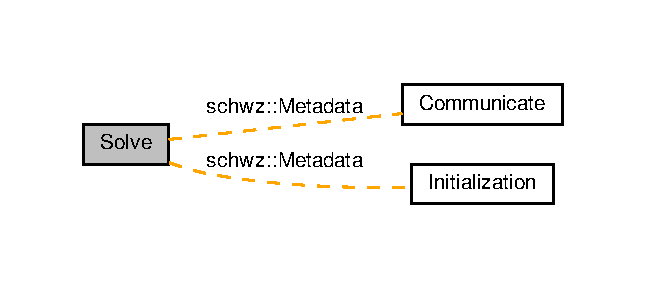
\includegraphics[width=310pt]{group__solve}
\end{center}
\end{figure}
\subsection*{Namespaces}
\begin{DoxyCompactItemize}
\item 
 \hyperlink{namespaceschwz_1_1ConvergenceTools}{schwz\+::\+Convergence\+Tools}
\begin{DoxyCompactList}\small\item\em The \hyperlink{namespaceschwz_1_1ConvergenceTools}{Convergence\+Tools} namespace . \end{DoxyCompactList}\item 
 \hyperlink{namespaceschwz_1_1SolverTools}{schwz\+::\+Solver\+Tools}
\begin{DoxyCompactList}\small\item\em The \hyperlink{namespaceschwz_1_1SolverTools}{Solver\+Tools} namespace . \end{DoxyCompactList}\end{DoxyCompactItemize}
\subsection*{Classes}
\begin{DoxyCompactItemize}
\item 
struct \hyperlink{structschwz_1_1Metadata}{schwz\+::\+Metadata$<$ Value\+Type, Index\+Type $>$}
\begin{DoxyCompactList}\small\item\em The solver metadata struct. \end{DoxyCompactList}\item 
class \hyperlink{classschwz_1_1Solve}{schwz\+::\+Solve$<$ Value\+Type, Index\+Type $>$}
\begin{DoxyCompactList}\small\item\em The Solver class the provides the solver and the convergence checking methods. \end{DoxyCompactList}\end{DoxyCompactItemize}


\subsection{Detailed Description}
A module dedicated to the solvers including local solution and convergence detection in schwarz-\/lib. 


\hypertarget{group__utils}{}\section{Utils}
\label{group__utils}\index{Utils@{Utils}}


A module dedicated to the utilities in schwarz-\/lib.  


\subsection*{Classes}
\begin{DoxyCompactItemize}
\item 
struct \hyperlink{structSchwarzWrappers_1_1Utils}{Schwarz\+Wrappers\+::\+Utils$<$ Value\+Type, Index\+Type $>$}
\begin{DoxyCompactList}\small\item\em The utilities class which provides some checks and basic utilities. \end{DoxyCompactList}\end{DoxyCompactItemize}


\subsection{Detailed Description}
A module dedicated to the utilities in schwarz-\/lib. 


\chapter{Namespace Documentation}
\hypertarget{namespaceProcessTopology}{}\section{Process\+Topology Namespace Reference}
\label{namespaceProcessTopology}\index{Process\+Topology@{Process\+Topology}}


The \hyperlink{namespaceProcessTopology}{Process\+Topology} namespace .  




\subsection{Detailed Description}
The \hyperlink{namespaceProcessTopology}{Process\+Topology} namespace . 

proc\+\_\+topo 
\hypertarget{namespaceschwz}{}\section{schwz Namespace Reference}
\label{namespaceschwz}\index{schwz@{schwz}}


The Schwarz wrappers namespace.  


\subsection*{Namespaces}
\begin{DoxyCompactItemize}
\item 
 \hyperlink{namespaceschwz_1_1CommHelpers}{Comm\+Helpers}
\begin{DoxyCompactList}\small\item\em The Comm\+Helper namespace . \end{DoxyCompactList}\item 
 \hyperlink{namespaceschwz_1_1conv__tools}{conv\+\_\+tools}
\begin{DoxyCompactList}\small\item\em The \hyperlink{namespaceschwz_1_1conv__tools}{conv\+\_\+tools} namespace . \end{DoxyCompactList}\item 
 \hyperlink{namespaceschwz_1_1PartitionTools}{Partition\+Tools}
\begin{DoxyCompactList}\small\item\em The \hyperlink{namespaceschwz_1_1PartitionTools}{Partition\+Tools} namespace . \end{DoxyCompactList}\item 
 \hyperlink{namespaceschwz_1_1SolverTools}{Solver\+Tools}
\begin{DoxyCompactList}\small\item\em The \hyperlink{namespaceschwz_1_1SolverTools}{Solver\+Tools} namespace . \end{DoxyCompactList}\end{DoxyCompactItemize}
\subsection*{Classes}
\begin{DoxyCompactItemize}
\item 
class \hyperlink{classschwz_1_1Communicate}{Communicate}
\begin{DoxyCompactList}\small\item\em The communication class that provides the methods for the communication between the subdomains. \end{DoxyCompactList}\item 
class \hyperlink{classschwz_1_1device__guard}{device\+\_\+guard}
\begin{DoxyCompactList}\small\item\em This class defines a device guard for the cuda functions and the cuda module. \end{DoxyCompactList}\item 
class \hyperlink{classschwz_1_1Initialize}{Initialize}
\begin{DoxyCompactList}\small\item\em The initialization class that provides methods for initialization of the solver. \end{DoxyCompactList}\item 
struct \hyperlink{structschwz_1_1Metadata}{Metadata}
\begin{DoxyCompactList}\small\item\em The solver metadata struct. \end{DoxyCompactList}\item 
class \hyperlink{classschwz_1_1SchwarzBase}{Schwarz\+Base}
\begin{DoxyCompactList}\small\item\em The Base solver class is meant to be the class implementing the common implementations for all the schwarz methods. \end{DoxyCompactList}\item 
struct \hyperlink{structschwz_1_1Settings}{Settings}
\begin{DoxyCompactList}\small\item\em The struct that contains the solver settings and the parameters to be set by the user. \end{DoxyCompactList}\item 
class \hyperlink{classschwz_1_1Solve}{Solve}
\begin{DoxyCompactList}\small\item\em The Solver class the provides the solver and the convergence checking methods. \end{DoxyCompactList}\item 
class \hyperlink{classschwz_1_1SolverRAS}{Solver\+R\+AS}
\begin{DoxyCompactList}\small\item\em An implementation of the solver interface using the R\+AS solver. \end{DoxyCompactList}\item 
struct \hyperlink{structschwz_1_1Utils}{Utils}
\begin{DoxyCompactList}\small\item\em The utilities class which provides some checks and basic utilities. \end{DoxyCompactList}\end{DoxyCompactItemize}
\subsection*{Functions}
\begin{DoxyCompactItemize}
\item 
\mbox{\Hypertarget{namespaceschwz_a443a272fc6c66825dc7a958e824e32e3}\label{namespaceschwz_a443a272fc6c66825dc7a958e824e32e3}} 
gko\+::size\+\_\+type {\bfseries linearize\+\_\+index} (const gko\+::size\+\_\+type row, const gko\+::size\+\_\+type col, const gko\+::size\+\_\+type num\+\_\+rows)
\item 
\mbox{\Hypertarget{namespaceschwz_a4c99059ae93f77311f4a14d28774c0d3}\label{namespaceschwz_a4c99059ae93f77311f4a14d28774c0d3}} 
{\footnotesize template$<$typename Value\+Type , typename Index\+Type , typename Mixed\+Value\+Type $>$ }\\void {\bfseries exchange\+\_\+boundary\+\_\+onesided} (const \hyperlink{structschwz_1_1Settings}{Settings} \&settings, const \hyperlink{structschwz_1_1Metadata}{Metadata}$<$ Value\+Type, Index\+Type $>$ \&metadata, struct \hyperlink{classschwz_1_1Communicate}{Communicate}$<$ Value\+Type, Index\+Type, Mixed\+Value\+Type $>$\+::comm\+\_\+struct \&comm\+\_\+struct, std\+::shared\+\_\+ptr$<$ gko\+::matrix\+::\+Dense$<$ Value\+Type $>$$>$ \&global\+\_\+solution)
\item 
\mbox{\Hypertarget{namespaceschwz_a5c58f9da7e21d6671295b7b62f45b33f}\label{namespaceschwz_a5c58f9da7e21d6671295b7b62f45b33f}} 
{\footnotesize template$<$typename Value\+Type , typename Index\+Type , typename Mixed\+Value\+Type $>$ }\\void {\bfseries exchange\+\_\+boundary\+\_\+twosided} (const \hyperlink{structschwz_1_1Settings}{Settings} \&settings, const \hyperlink{structschwz_1_1Metadata}{Metadata}$<$ Value\+Type, Index\+Type $>$ \&metadata, struct \hyperlink{classschwz_1_1Communicate}{Communicate}$<$ Value\+Type, Index\+Type, Mixed\+Value\+Type $>$\+::comm\+\_\+struct \&comm\+\_\+struct, std\+::shared\+\_\+ptr$<$ gko\+::matrix\+::\+Dense$<$ Value\+Type $>$$>$ \&global\+\_\+solution)
\item 
\mbox{\Hypertarget{namespaceschwz_af5437b273e3d364a2b3fa80929aeded9}\label{namespaceschwz_af5437b273e3d364a2b3fa80929aeded9}} 
{\footnotesize template$<$typename Value\+Type , typename Index\+Type $>$ }\\void {\bfseries write\+\_\+iters\+\_\+and\+\_\+residuals} (int num\+\_\+subd, int my\+\_\+rank, int iter\+\_\+count, std\+::vector$<$ Value\+Type $>$ \&local\+\_\+res\+\_\+vec\+\_\+out, std\+::vector$<$ Index\+Type $>$ \&local\+\_\+converged\+\_\+iter\+\_\+count, std\+::vector$<$ Value\+Type $>$ \&local\+\_\+converged\+\_\+resnorm, std\+::vector$<$ Value\+Type $>$ \&local\+\_\+timestamp, std\+::string filename)
\item 
\mbox{\Hypertarget{namespaceschwz_a6e174da7b0a888de0b361c6ef27ae10a}\label{namespaceschwz_a6e174da7b0a888de0b361c6ef27ae10a}} 
{\footnotesize template$<$typename Value\+Type , typename Index\+Type , typename Mixed\+Value\+Type $>$ }\\void {\bfseries gather\+\_\+comm\+\_\+data} (int num\+\_\+subdomains, struct \hyperlink{classschwz_1_1Communicate}{Communicate}$<$ Value\+Type, Index\+Type, Mixed\+Value\+Type $>$\+::comm\+\_\+struct \&comm\+\_\+struct, std\+::vector$<$ std\+::tuple$<$ int, std\+::vector$<$ std\+::tuple$<$ int, int $>$$>$, std\+::vector$<$ std\+::tuple$<$ int, int $>$$>$, int, int $>$$>$ \&comm\+\_\+data\+\_\+struct)
\item 
\mbox{\Hypertarget{namespaceschwz_a326d36155d6eeccd87f66fdf5200df29}\label{namespaceschwz_a326d36155d6eeccd87f66fdf5200df29}} 
{\footnotesize template$<$typename Value\+Type $>$ }\\double {\bfseries get\+\_\+relative\+\_\+error} (const gko\+::matrix\+::\+Dense$<$ Value\+Type $>$ $\ast$first, const gko\+::matrix\+::\+Dense$<$ Value\+Type $>$ $\ast$second)
\item 
\mbox{\Hypertarget{namespaceschwz_aac5839ef31d9d40a6a9c80a8611b6e50}\label{namespaceschwz_aac5839ef31d9d40a6a9c80a8611b6e50}} 
{\footnotesize template$<$typename Value\+Type , typename Index\+Type $>$ }\\void {\bfseries update\+\_\+diagonals} (std\+::shared\+\_\+ptr$<$ gko\+::matrix\+::\+Csr$<$ Value\+Type, Index\+Type $>$$>$ \&matrix, std\+::vector$<$ Value\+Type $>$ \&diags)
\end{DoxyCompactItemize}


\subsection{Detailed Description}
The Schwarz wrappers namespace. 
\hypertarget{namespaceschwz_1_1CommHelpers}{}\section{schwz\+:\+:Comm\+Helpers Namespace Reference}
\label{namespaceschwz_1_1CommHelpers}\index{schwz\+::\+Comm\+Helpers@{schwz\+::\+Comm\+Helpers}}


The Comm\+Helper namespace .  


\subsection*{Functions}
\begin{DoxyCompactItemize}
\item 
\mbox{\Hypertarget{namespaceschwz_1_1CommHelpers_a2ec36b7c44dc5aa2650fa2aedbfa0f93}\label{namespaceschwz_1_1CommHelpers_a2ec36b7c44dc5aa2650fa2aedbfa0f93}} 
{\footnotesize template$<$typename Value\+Type , typename Index\+Type $>$ }\\void {\bfseries transfer\+\_\+one\+\_\+by\+\_\+one} (const \hyperlink{structschwz_1_1Settings}{Settings} \&settings, M\+P\+I\+\_\+\+Win \&window, Value\+Type $\ast$buffer, Index\+Type $\ast$$\ast$offset, const int num\+\_\+neighbors, const Index\+Type $\ast$neighbors)
\item 
\mbox{\Hypertarget{namespaceschwz_1_1CommHelpers_a4407510891fd56c91940d8ff12e172d9}\label{namespaceschwz_1_1CommHelpers_a4407510891fd56c91940d8ff12e172d9}} 
{\footnotesize template$<$typename Value\+Type , typename Index\+Type $>$ }\\void {\bfseries pack\+\_\+buffer} (const \hyperlink{structschwz_1_1Settings}{Settings} \&settings, Value\+Type $\ast$buffer, Value\+Type $\ast$send\+\_\+buffer, Value\+Type $\ast$work\+\_\+vector, Index\+Type $\ast$$\ast$num\+\_\+send\+\_\+elems, const int offset, const int send\+\_\+subd, std\+::vector$<$ bool $>$ \&is\+\_\+local\+\_\+neighbor)
\item 
\mbox{\Hypertarget{namespaceschwz_1_1CommHelpers_a50ed2dd8908c8d6a42ed4149fcaa0bb0}\label{namespaceschwz_1_1CommHelpers_a50ed2dd8908c8d6a42ed4149fcaa0bb0}} 
{\footnotesize template$<$typename Value\+Type , typename Index\+Type $>$ }\\void {\bfseries transfer\+\_\+buffer} (const \hyperlink{structschwz_1_1Settings}{Settings} \&settings, M\+P\+I\+\_\+\+Win \&window, Value\+Type $\ast$target\+\_\+buffer, Index\+Type $\ast$$\ast$num\+\_\+elems, const int offset, const int target\+\_\+subd, const Index\+Type $\ast$neighbors, const Index\+Type $\ast$displacements)
\item 
\mbox{\Hypertarget{namespaceschwz_1_1CommHelpers_ac841a73655ae4b95495192709730563c}\label{namespaceschwz_1_1CommHelpers_ac841a73655ae4b95495192709730563c}} 
{\footnotesize template$<$typename Value\+Type , typename Index\+Type $>$ }\\void {\bfseries unpack\+\_\+buffer} (const \hyperlink{structschwz_1_1Settings}{Settings} \&settings, Value\+Type $\ast$buffer, Value\+Type $\ast$recv\+\_\+buffer, Value\+Type $\ast$work\+\_\+vector, Index\+Type $\ast$$\ast$num\+\_\+recv\+\_\+elems, const int offset, const int recv\+\_\+subd, std\+::vector$<$ bool $>$ \&is\+\_\+local\+\_\+neighbor)
\end{DoxyCompactItemize}


\subsection{Detailed Description}
The Comm\+Helper namespace . 

comm\+\_\+helpers 
\hypertarget{namespaceschwz_1_1conv__tools}{}\section{schwz\+:\+:conv\+\_\+tools Namespace Reference}
\label{namespaceschwz_1_1conv__tools}\index{schwz\+::conv\+\_\+tools@{schwz\+::conv\+\_\+tools}}


The \hyperlink{namespaceschwz_1_1conv__tools}{conv\+\_\+tools} namespace .  


\subsection*{Functions}
\begin{DoxyCompactItemize}
\item 
\mbox{\Hypertarget{namespaceschwz_1_1conv__tools_a36a12a05164af19e0faec5403fd3cfce}\label{namespaceschwz_1_1conv__tools_a36a12a05164af19e0faec5403fd3cfce}} 
{\footnotesize template$<$typename Value\+Type , typename Index\+Type $>$ }\\void {\bfseries put\+\_\+all\+\_\+local\+\_\+residual\+\_\+norms} (const \hyperlink{structschwz_1_1Settings}{Settings} \&settings, \hyperlink{structschwz_1_1Metadata}{Metadata}$<$ Value\+Type, Index\+Type $>$ \&metadata, Value\+Type \&local\+\_\+resnorm, std\+::shared\+\_\+ptr$<$ gko\+::matrix\+::\+Dense$<$ Value\+Type $>$$>$ \&local\+\_\+residual\+\_\+vector, M\+P\+I\+\_\+\+Win \&window\+\_\+residual\+\_\+vector)
\item 
\mbox{\Hypertarget{namespaceschwz_1_1conv__tools_a8e33cee5af118a993c675464124aa6d6}\label{namespaceschwz_1_1conv__tools_a8e33cee5af118a993c675464124aa6d6}} 
{\footnotesize template$<$typename Value\+Type , typename Index\+Type $>$ }\\void {\bfseries propagate\+\_\+all\+\_\+local\+\_\+residual\+\_\+norms} (const \hyperlink{structschwz_1_1Settings}{Settings} \&settings, \hyperlink{structschwz_1_1Metadata}{Metadata}$<$ Value\+Type, Index\+Type $>$ \&metadata, struct \hyperlink{classschwz_1_1Communicate}{Communicate}$<$ Value\+Type, Index\+Type $>$\+::comm\+\_\+struct \&comm\+\_\+s, Value\+Type \&local\+\_\+resnorm, std\+::shared\+\_\+ptr$<$ gko\+::matrix\+::\+Dense$<$ Value\+Type $>$$>$ \&local\+\_\+residual\+\_\+vector, M\+P\+I\+\_\+\+Win \&window\+\_\+residual\+\_\+vector)
\item 
\mbox{\Hypertarget{namespaceschwz_1_1conv__tools_ad2a454563a99665373863676ab9c0a72}\label{namespaceschwz_1_1conv__tools_ad2a454563a99665373863676ab9c0a72}} 
{\footnotesize template$<$typename Value\+Type , typename Index\+Type $>$ }\\void {\bfseries global\+\_\+convergence\+\_\+check\+\_\+onesided\+\_\+tree} (const \hyperlink{structschwz_1_1Settings}{Settings} \&settings, const \hyperlink{structschwz_1_1Metadata}{Metadata}$<$ Value\+Type, Index\+Type $>$ \&metadata, std\+::shared\+\_\+ptr$<$ gko\+::\+Array$<$ Index\+Type $>$$>$ \&convergence\+\_\+vector, int \&converged\+\_\+all\+\_\+local, int \&num\+\_\+converged\+\_\+procs, M\+P\+I\+\_\+\+Win \&window\+\_\+convergence)
\item 
\mbox{\Hypertarget{namespaceschwz_1_1conv__tools_a84a9cec6599d333ee2382ab54a8ce819}\label{namespaceschwz_1_1conv__tools_a84a9cec6599d333ee2382ab54a8ce819}} 
{\footnotesize template$<$typename Value\+Type , typename Index\+Type $>$ }\\void {\bfseries global\+\_\+convergence\+\_\+decentralized} (const \hyperlink{structschwz_1_1Settings}{Settings} \&settings, const \hyperlink{structschwz_1_1Metadata}{Metadata}$<$ Value\+Type, Index\+Type $>$ \&metadata, struct \hyperlink{classschwz_1_1Communicate}{Communicate}$<$ Value\+Type, Index\+Type $>$\+::comm\+\_\+struct \&comm\+\_\+s, std\+::shared\+\_\+ptr$<$ gko\+::\+Array$<$ Index\+Type $>$$>$ \&convergence\+\_\+vector, std\+::shared\+\_\+ptr$<$ gko\+::\+Array$<$ Index\+Type $>$$>$ \&convergence\+\_\+sent, std\+::shared\+\_\+ptr$<$ gko\+::\+Array$<$ Index\+Type $>$$>$ \&convergence\+\_\+local, int \&converged\+\_\+all\+\_\+local, int \&num\+\_\+converged\+\_\+procs, M\+P\+I\+\_\+\+Win \&window\+\_\+convergence)
\end{DoxyCompactItemize}


\subsection{Detailed Description}
The \hyperlink{namespaceschwz_1_1conv__tools}{conv\+\_\+tools} namespace . 

\hyperlink{namespaceschwz_1_1conv__tools}{conv\+\_\+tools} 
\hypertarget{namespaceschwz_1_1EventHelpers}{}\section{schwz\+:\+:Event\+Helpers Namespace Reference}
\label{namespaceschwz_1_1EventHelpers}\index{schwz\+::\+Event\+Helpers@{schwz\+::\+Event\+Helpers}}


The Event\+Helper namespace .  


\subsection*{Functions}
\begin{DoxyCompactItemize}
\item 
\mbox{\Hypertarget{namespaceschwz_1_1EventHelpers_af3426fb8505cc11bb5eeb9ec14a61b2a}\label{namespaceschwz_1_1EventHelpers_af3426fb8505cc11bb5eeb9ec14a61b2a}} 
{\footnotesize template$<$typename Value\+Type , typename Index\+Type , typename Mixed\+Value\+Type $>$ }\\Value\+Type {\bfseries compute\+\_\+nonadaptive\+\_\+threshold} (const \hyperlink{structschwz_1_1Settings}{Settings} \&settings, const \hyperlink{structschwz_1_1Metadata}{Metadata}$<$ Value\+Type, Index\+Type $>$ \&metadata)
\item 
\mbox{\Hypertarget{namespaceschwz_1_1EventHelpers_a8b0ef495ae54545747b8caf0d25aaaef}\label{namespaceschwz_1_1EventHelpers_a8b0ef495ae54545747b8caf0d25aaaef}} 
{\footnotesize template$<$typename Value\+Type , typename Index\+Type , typename Mixed\+Value\+Type $>$ }\\Value\+Type {\bfseries compute\+\_\+adaptive\+\_\+threshold} (const \hyperlink{structschwz_1_1Settings}{Settings} \&settings, const \hyperlink{structschwz_1_1Metadata}{Metadata}$<$ Value\+Type, Index\+Type $>$ \&metadata, struct \hyperlink{classschwz_1_1Communicate}{Communicate}$<$ Value\+Type, Index\+Type, Mixed\+Value\+Type $>$\+::comm\+\_\+struct \&comm\+\_\+struct, int target\+\_\+subd, int iter\+\_\+diff)
\item 
\mbox{\Hypertarget{namespaceschwz_1_1EventHelpers_a908e89a6f642e50e3be947411613a8bf}\label{namespaceschwz_1_1EventHelpers_a908e89a6f642e50e3be947411613a8bf}} 
{\footnotesize template$<$typename Value\+Type , typename Index\+Type , typename Mixed\+Value\+Type $>$ }\\void {\bfseries compute\+\_\+sender\+\_\+slopes} (const \hyperlink{structschwz_1_1Settings}{Settings} \&settings, const \hyperlink{structschwz_1_1Metadata}{Metadata}$<$ Value\+Type, Index\+Type $>$ \&metadata, struct \hyperlink{classschwz_1_1Communicate}{Communicate}$<$ Value\+Type, Index\+Type, Mixed\+Value\+Type $>$\+::comm\+\_\+struct \&comm\+\_\+struct, int target\+\_\+subd, int iter\+\_\+diff, Value\+Type value\+\_\+diff)
\item 
\mbox{\Hypertarget{namespaceschwz_1_1EventHelpers_a8b4074a3854542790fe7e71da7680ed3}\label{namespaceschwz_1_1EventHelpers_a8b4074a3854542790fe7e71da7680ed3}} 
{\footnotesize template$<$typename Value\+Type , typename Index\+Type , typename Mixed\+Value\+Type $>$ }\\void {\bfseries compute\+\_\+receiver\+\_\+slopes} (const \hyperlink{structschwz_1_1Settings}{Settings} \&settings, const \hyperlink{structschwz_1_1Metadata}{Metadata}$<$ Value\+Type, Index\+Type $>$ \&metadata, struct \hyperlink{classschwz_1_1Communicate}{Communicate}$<$ Value\+Type, Index\+Type, Mixed\+Value\+Type $>$\+::comm\+\_\+struct \&comm\+\_\+struct, int target\+\_\+subd, int iter\+\_\+diff, int num\+\_\+get)
\item 
\mbox{\Hypertarget{namespaceschwz_1_1EventHelpers_a750dc14b8dcf40cbefc915ae42ea6fa7}\label{namespaceschwz_1_1EventHelpers_a750dc14b8dcf40cbefc915ae42ea6fa7}} 
{\footnotesize template$<$typename Value\+Type , typename Index\+Type , typename Mixed\+Value\+Type $>$ }\\Value\+Type {\bfseries generate\+\_\+extrapolated\+\_\+buffer} (const \hyperlink{structschwz_1_1Settings}{Settings} \&settings, const \hyperlink{structschwz_1_1Metadata}{Metadata}$<$ Value\+Type, Index\+Type $>$ \&metadata, struct \hyperlink{classschwz_1_1Communicate}{Communicate}$<$ Value\+Type, Index\+Type, Mixed\+Value\+Type $>$\+::comm\+\_\+struct \&comm\+\_\+struct, int target\+\_\+subd, int iter\+\_\+diff, int num\+\_\+get)
\end{DoxyCompactItemize}


\subsection{Detailed Description}
The Event\+Helper namespace . 

event\+\_\+helpers 
\hypertarget{namespaceschwz_1_1PartitionTools}{}\section{schwz\+:\+:Partition\+Tools Namespace Reference}
\label{namespaceschwz_1_1PartitionTools}\index{schwz\+::\+Partition\+Tools@{schwz\+::\+Partition\+Tools}}


The \hyperlink{namespaceschwz_1_1PartitionTools}{Partition\+Tools} namespace .  


\subsection*{Functions}
\begin{DoxyCompactItemize}
\item 
\mbox{\Hypertarget{namespaceschwz_1_1PartitionTools_a8704c901dcdadbe942f2efbe118b3755}\label{namespaceschwz_1_1PartitionTools_a8704c901dcdadbe942f2efbe118b3755}} 
{\footnotesize template$<$typename Value\+Type , typename Index\+Type $>$ }\\void {\bfseries Partition\+Regular} (const std\+::shared\+\_\+ptr$<$ gko\+::matrix\+::\+Csr$<$ Value\+Type, Index\+Type $>$$>$ \&global\+\_\+matrix, const unsigned int \&n\+\_\+partitions, std\+::vector$<$ unsigned int $>$ \&partition\+\_\+indices)
\item 
\mbox{\Hypertarget{namespaceschwz_1_1PartitionTools_ab7e001c062718aa83b5a4be768c10278}\label{namespaceschwz_1_1PartitionTools_ab7e001c062718aa83b5a4be768c10278}} 
{\footnotesize template$<$typename Value\+Type , typename Index\+Type $>$ }\\void {\bfseries Partition\+Regular2D} (const std\+::shared\+\_\+ptr$<$ gko\+::matrix\+::\+Csr$<$ Value\+Type, Index\+Type $>$$>$ \&global\+\_\+matrix, bool write\+\_\+debug\+\_\+out, const unsigned int \&n\+\_\+partitions, std\+::vector$<$ unsigned int $>$ \&partition\+\_\+indices)
\item 
\mbox{\Hypertarget{namespaceschwz_1_1PartitionTools_ad29c7a2a6d130f422f7333886c53332c}\label{namespaceschwz_1_1PartitionTools_ad29c7a2a6d130f422f7333886c53332c}} 
{\footnotesize template$<$typename Value\+Type , typename Index\+Type $>$ }\\void {\bfseries Partition\+Metis} (const \hyperlink{structschwz_1_1Settings}{Settings} \&settings, const std\+::shared\+\_\+ptr$<$ gko\+::matrix\+::\+Csr$<$ Value\+Type, Index\+Type $>$$>$ \&global\+\_\+matrix, const std\+::vector$<$ unsigned int $>$ \&cell\+\_\+weights, const unsigned int \&n\+\_\+partitions, std\+::vector$<$ unsigned int $>$ \&partition\+\_\+indices)
\item 
\mbox{\Hypertarget{namespaceschwz_1_1PartitionTools_ad329e178d7e0ff9228dbec6714fcea45}\label{namespaceschwz_1_1PartitionTools_ad329e178d7e0ff9228dbec6714fcea45}} 
template void {\bfseries Partition\+Metis} (const \hyperlink{structschwz_1_1Settings}{Settings} \&, const std\+::shared\+\_\+ptr$<$ gko\+::matrix\+::\+Csr$<$ float, gko\+::int32 $>$$>$ \&, const std\+::vector$<$ unsigned int $>$ \&, const unsigned int \&, std\+::vector$<$ unsigned int $>$ \&)
\item 
\mbox{\Hypertarget{namespaceschwz_1_1PartitionTools_ab8f4fc729053b01f737fa88c06c5595f}\label{namespaceschwz_1_1PartitionTools_ab8f4fc729053b01f737fa88c06c5595f}} 
template void {\bfseries Partition\+Metis} (const \hyperlink{structschwz_1_1Settings}{Settings} \&, const std\+::shared\+\_\+ptr$<$ gko\+::matrix\+::\+Csr$<$ double, gko\+::int32 $>$$>$ \&, const std\+::vector$<$ unsigned int $>$ \&, const unsigned int \&, std\+::vector$<$ unsigned int $>$ \&)
\item 
\mbox{\Hypertarget{namespaceschwz_1_1PartitionTools_a5a1fe167c67313ecad2a2aa4546c22a3}\label{namespaceschwz_1_1PartitionTools_a5a1fe167c67313ecad2a2aa4546c22a3}} 
template void {\bfseries Partition\+Metis} (const \hyperlink{structschwz_1_1Settings}{Settings} \&, const std\+::shared\+\_\+ptr$<$ gko\+::matrix\+::\+Csr$<$ float, gko\+::int64 $>$$>$ \&, const std\+::vector$<$ unsigned int $>$ \&, const unsigned int \&, std\+::vector$<$ unsigned int $>$ \&)
\item 
\mbox{\Hypertarget{namespaceschwz_1_1PartitionTools_aaedda6a3597838a57a516429662048fb}\label{namespaceschwz_1_1PartitionTools_aaedda6a3597838a57a516429662048fb}} 
template void {\bfseries Partition\+Metis} (const \hyperlink{structschwz_1_1Settings}{Settings} \&, const std\+::shared\+\_\+ptr$<$ gko\+::matrix\+::\+Csr$<$ double, gko\+::int64 $>$$>$ \&, const std\+::vector$<$ unsigned int $>$ \&, const unsigned int \&, std\+::vector$<$ unsigned int $>$ \&)
\item 
\mbox{\Hypertarget{namespaceschwz_1_1PartitionTools_afe31b63fd24048da65807e684b809185}\label{namespaceschwz_1_1PartitionTools_afe31b63fd24048da65807e684b809185}} 
template void {\bfseries Partition\+Regular} (const std\+::shared\+\_\+ptr$<$ gko\+::matrix\+::\+Csr$<$ float, gko\+::int32 $>$$>$ \&, const unsigned int \&, std\+::vector$<$ unsigned int $>$ \&)
\item 
\mbox{\Hypertarget{namespaceschwz_1_1PartitionTools_a7b90a8fb50162839c76afddae52331a4}\label{namespaceschwz_1_1PartitionTools_a7b90a8fb50162839c76afddae52331a4}} 
template void {\bfseries Partition\+Regular} (const std\+::shared\+\_\+ptr$<$ gko\+::matrix\+::\+Csr$<$ double, gko\+::int32 $>$$>$ \&, const unsigned int \&, std\+::vector$<$ unsigned int $>$ \&)
\item 
\mbox{\Hypertarget{namespaceschwz_1_1PartitionTools_ae309b46e40996539cab104b01e671af8}\label{namespaceschwz_1_1PartitionTools_ae309b46e40996539cab104b01e671af8}} 
template void {\bfseries Partition\+Regular} (const std\+::shared\+\_\+ptr$<$ gko\+::matrix\+::\+Csr$<$ float, gko\+::int64 $>$$>$ \&, const unsigned int \&, std\+::vector$<$ unsigned int $>$ \&)
\item 
\mbox{\Hypertarget{namespaceschwz_1_1PartitionTools_ac5e6e7e957a85bc5c10ddd051300a3bb}\label{namespaceschwz_1_1PartitionTools_ac5e6e7e957a85bc5c10ddd051300a3bb}} 
template void {\bfseries Partition\+Regular} (const std\+::shared\+\_\+ptr$<$ gko\+::matrix\+::\+Csr$<$ double, gko\+::int64 $>$$>$ \&, const unsigned int \&, std\+::vector$<$ unsigned int $>$ \&)
\end{DoxyCompactItemize}


\subsection{Detailed Description}
The \hyperlink{namespaceschwz_1_1PartitionTools}{Partition\+Tools} namespace . 

part\+\_\+tools 
\hypertarget{namespaceschwz_1_1SolverTools}{}\section{schwz\+:\+:Solver\+Tools Namespace Reference}
\label{namespaceschwz_1_1SolverTools}\index{schwz\+::\+Solver\+Tools@{schwz\+::\+Solver\+Tools}}


The \hyperlink{namespaceschwz_1_1SolverTools}{Solver\+Tools} namespace .  


\subsection*{Functions}
\begin{DoxyCompactItemize}
\item 
\mbox{\Hypertarget{namespaceschwz_1_1SolverTools_ae0eb9798ac886b0e45c304a97fe70176}\label{namespaceschwz_1_1SolverTools_ae0eb9798ac886b0e45c304a97fe70176}} 
{\footnotesize template$<$typename Value\+Type , typename Index\+Type $>$ }\\void {\bfseries solve\+\_\+direct\+\_\+ginkgo} (const \hyperlink{structschwz_1_1Settings}{Settings} \&settings, const \hyperlink{structschwz_1_1Metadata}{Metadata}$<$ Value\+Type, Index\+Type $>$ \&metadata, const std\+::shared\+\_\+ptr$<$ gko\+::solver\+::\+Lower\+Trs$<$ Value\+Type, Index\+Type $>$$>$ \&L\+\_\+solver, const std\+::shared\+\_\+ptr$<$ gko\+::solver\+::\+Upper\+Trs$<$ Value\+Type, Index\+Type $>$$>$ \&U\+\_\+solver, std\+::shared\+\_\+ptr$<$ gko\+::matrix\+::\+Dense$<$ Value\+Type $>$$>$ \&work\+\_\+vector, std\+::shared\+\_\+ptr$<$ gko\+::matrix\+::\+Dense$<$ Value\+Type $>$$>$ \&local\+\_\+solution)
\item 
\mbox{\Hypertarget{namespaceschwz_1_1SolverTools_a246fa524f65b66c548ecd16a74124356}\label{namespaceschwz_1_1SolverTools_a246fa524f65b66c548ecd16a74124356}} 
{\footnotesize template$<$typename Value\+Type , typename Index\+Type $>$ }\\void {\bfseries solve\+\_\+iterative\+\_\+ginkgo} (const \hyperlink{structschwz_1_1Settings}{Settings} \&settings, const \hyperlink{structschwz_1_1Metadata}{Metadata}$<$ Value\+Type, Index\+Type $>$ \&metadata, const std\+::shared\+\_\+ptr$<$ gko\+::\+Lin\+Op $>$ \&solver, const std\+::shared\+\_\+ptr$<$ gko\+::matrix\+::\+Dense$<$ Value\+Type $>$$>$ \&local\+\_\+rhs, std\+::shared\+\_\+ptr$<$ gko\+::matrix\+::\+Dense$<$ Value\+Type $>$$>$ \&local\+\_\+solution)
\item 
\mbox{\Hypertarget{namespaceschwz_1_1SolverTools_a193e789c220cc7675b4cd7da073f3779}\label{namespaceschwz_1_1SolverTools_a193e789c220cc7675b4cd7da073f3779}} 
{\footnotesize template$<$typename Value\+Type , typename Index\+Type $>$ }\\void {\bfseries extract\+\_\+local\+\_\+vector} (const \hyperlink{structschwz_1_1Settings}{Settings} \&settings, const \hyperlink{structschwz_1_1Metadata}{Metadata}$<$ Value\+Type, Index\+Type $>$ \&metadata, gko\+::matrix\+::\+Dense$<$ Value\+Type $>$ $\ast$sub\+\_\+vector, const gko\+::matrix\+::\+Dense$<$ Value\+Type $>$ $\ast$vector, const Index\+Type \&vec\+\_\+index)
\end{DoxyCompactItemize}


\subsection{Detailed Description}
The \hyperlink{namespaceschwz_1_1SolverTools}{Solver\+Tools} namespace . 

solver\+\_\+tools 
\chapter{Class Documentation}
\hypertarget{classBadDimension}{}\section{Bad\+Dimension Class Reference}
\label{classBadDimension}\index{Bad\+Dimension@{Bad\+Dimension}}


\hyperlink{classBadDimension}{Bad\+Dimension} is thrown if an operation is being applied to a Lin\+Op with bad dimensions.  




{\ttfamily \#include $<$exception.\+hpp$>$}



Collaboration diagram for Bad\+Dimension\+:
\nopagebreak
\begin{figure}[H]
\begin{center}
\leavevmode
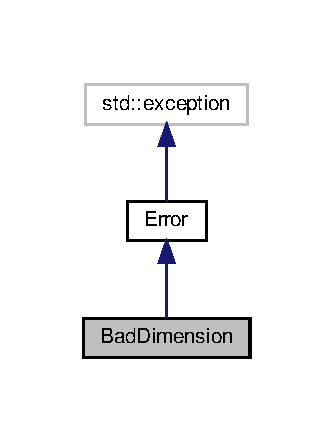
\includegraphics[width=160pt]{classBadDimension__coll__graph}
\end{center}
\end{figure}
\subsection*{Public Member Functions}
\begin{DoxyCompactItemize}
\item 
\hyperlink{classBadDimension_a4868c7892d3879a155f37daf04b7f8e9}{Bad\+Dimension} (const std\+::string \&file, int line, const std\+::string \&func, const std\+::string \&op\+\_\+name, std\+::size\+\_\+t op\+\_\+num\+\_\+rows, std\+::size\+\_\+t op\+\_\+num\+\_\+cols, const std\+::string \&clarification)
\begin{DoxyCompactList}\small\item\em Initializes a bad dimension error. \end{DoxyCompactList}\end{DoxyCompactItemize}


\subsection{Detailed Description}
\hyperlink{classBadDimension}{Bad\+Dimension} is thrown if an operation is being applied to a Lin\+Op with bad dimensions. 

\subsection{Constructor \& Destructor Documentation}
\mbox{\Hypertarget{classBadDimension_a4868c7892d3879a155f37daf04b7f8e9}\label{classBadDimension_a4868c7892d3879a155f37daf04b7f8e9}} 
\index{Bad\+Dimension@{Bad\+Dimension}!Bad\+Dimension@{Bad\+Dimension}}
\index{Bad\+Dimension@{Bad\+Dimension}!Bad\+Dimension@{Bad\+Dimension}}
\subsubsection{\texorpdfstring{Bad\+Dimension()}{BadDimension()}}
{\footnotesize\ttfamily Bad\+Dimension\+::\+Bad\+Dimension (\begin{DoxyParamCaption}\item[{const std\+::string \&}]{file,  }\item[{int}]{line,  }\item[{const std\+::string \&}]{func,  }\item[{const std\+::string \&}]{op\+\_\+name,  }\item[{std\+::size\+\_\+t}]{op\+\_\+num\+\_\+rows,  }\item[{std\+::size\+\_\+t}]{op\+\_\+num\+\_\+cols,  }\item[{const std\+::string \&}]{clarification }\end{DoxyParamCaption})\hspace{0.3cm}{\ttfamily [inline]}}



Initializes a bad dimension error. 


\begin{DoxyParams}{Parameters}
{\em file} & The name of the offending source file \\
\hline
{\em line} & The source code line number where the error occurred \\
\hline
{\em func} & The function name where the error occurred \\
\hline
{\em op\+\_\+name} & The name of the operator \\
\hline
{\em op\+\_\+num\+\_\+rows} & The row dimension of the operator \\
\hline
{\em op\+\_\+num\+\_\+cols} & The column dimension of the operator \\
\hline
{\em clarification} & An additional message further describing the error \\
\hline
\end{DoxyParams}


The documentation for this class was generated from the following file\+:\begin{DoxyCompactItemize}
\item 
exception.\+hpp (57e6370)\end{DoxyCompactItemize}

\hypertarget{structschwz_1_1Settings_1_1comm__settings}{}\section{schwz\+:\+:Settings\+:\+:comm\+\_\+settings Struct Reference}
\label{structschwz_1_1Settings_1_1comm__settings}\index{schwz\+::\+Settings\+::comm\+\_\+settings@{schwz\+::\+Settings\+::comm\+\_\+settings}}


The settings for the various available communication paradigms.  




{\ttfamily \#include $<$settings.\+hpp$>$}

\subsection*{Public Attributes}
\begin{DoxyCompactItemize}
\item 
\mbox{\Hypertarget{structschwz_1_1Settings_1_1comm__settings_ad4273bd93cf3ee223c6c099a5fe9d02c}\label{structschwz_1_1Settings_1_1comm__settings_ad4273bd93cf3ee223c6c099a5fe9d02c}} 
bool \hyperlink{structschwz_1_1Settings_1_1comm__settings_ad4273bd93cf3ee223c6c099a5fe9d02c}{enable\+\_\+onesided} = false
\begin{DoxyCompactList}\small\item\em Enable one-\/sided communication. \end{DoxyCompactList}\item 
\mbox{\Hypertarget{structschwz_1_1Settings_1_1comm__settings_a6ddd499f563bc4463e117b4e4ad495e6}\label{structschwz_1_1Settings_1_1comm__settings_a6ddd499f563bc4463e117b4e4ad495e6}} 
bool \hyperlink{structschwz_1_1Settings_1_1comm__settings_a6ddd499f563bc4463e117b4e4ad495e6}{enable\+\_\+overlap} = false
\begin{DoxyCompactList}\small\item\em Enable explicit overlap between communication and computation. \end{DoxyCompactList}\item 
\mbox{\Hypertarget{structschwz_1_1Settings_1_1comm__settings_ad9b64e9c41ab52a3f58de7e190aabee0}\label{structschwz_1_1Settings_1_1comm__settings_ad9b64e9c41ab52a3f58de7e190aabee0}} 
bool \hyperlink{structschwz_1_1Settings_1_1comm__settings_ad9b64e9c41ab52a3f58de7e190aabee0}{enable\+\_\+put} = false
\begin{DoxyCompactList}\small\item\em Put the data to the window using M\+P\+I\+\_\+\+Put rather than get. \end{DoxyCompactList}\item 
\mbox{\Hypertarget{structschwz_1_1Settings_1_1comm__settings_ab14aa253c21562ebe91bf52f42731c19}\label{structschwz_1_1Settings_1_1comm__settings_ab14aa253c21562ebe91bf52f42731c19}} 
bool \hyperlink{structschwz_1_1Settings_1_1comm__settings_ab14aa253c21562ebe91bf52f42731c19}{enable\+\_\+get} = true
\begin{DoxyCompactList}\small\item\em Get the data to the window using M\+P\+I\+\_\+\+Get rather than put. \end{DoxyCompactList}\item 
\mbox{\Hypertarget{structschwz_1_1Settings_1_1comm__settings_aae063b9fcf2bc8e49e960286e4c0939f}\label{structschwz_1_1Settings_1_1comm__settings_aae063b9fcf2bc8e49e960286e4c0939f}} 
bool \hyperlink{structschwz_1_1Settings_1_1comm__settings_aae063b9fcf2bc8e49e960286e4c0939f}{enable\+\_\+one\+\_\+by\+\_\+one} = false
\begin{DoxyCompactList}\small\item\em Push each element separately directly into the buffer. \end{DoxyCompactList}\item 
\mbox{\Hypertarget{structschwz_1_1Settings_1_1comm__settings_a5bea917e0dc11a5a671bd4d8cdb3e3cf}\label{structschwz_1_1Settings_1_1comm__settings_a5bea917e0dc11a5a671bd4d8cdb3e3cf}} 
bool \hyperlink{structschwz_1_1Settings_1_1comm__settings_a5bea917e0dc11a5a671bd4d8cdb3e3cf}{enable\+\_\+flush\+\_\+local} = false
\begin{DoxyCompactList}\small\item\em Use local flush. \end{DoxyCompactList}\item 
\mbox{\Hypertarget{structschwz_1_1Settings_1_1comm__settings_a3eb62d22f79472020fce577ceddad916}\label{structschwz_1_1Settings_1_1comm__settings_a3eb62d22f79472020fce577ceddad916}} 
bool \hyperlink{structschwz_1_1Settings_1_1comm__settings_a3eb62d22f79472020fce577ceddad916}{enable\+\_\+flush\+\_\+all} = true
\begin{DoxyCompactList}\small\item\em Use flush all. \end{DoxyCompactList}\item 
\mbox{\Hypertarget{structschwz_1_1Settings_1_1comm__settings_abc715396bf51f36307caf88db02c819c}\label{structschwz_1_1Settings_1_1comm__settings_abc715396bf51f36307caf88db02c819c}} 
bool \hyperlink{structschwz_1_1Settings_1_1comm__settings_abc715396bf51f36307caf88db02c819c}{enable\+\_\+lock\+\_\+local} = false
\begin{DoxyCompactList}\small\item\em Use local locks. \end{DoxyCompactList}\item 
\mbox{\Hypertarget{structschwz_1_1Settings_1_1comm__settings_a39a59cea325ea1b57aba12e9ada4b91b}\label{structschwz_1_1Settings_1_1comm__settings_a39a59cea325ea1b57aba12e9ada4b91b}} 
bool \hyperlink{structschwz_1_1Settings_1_1comm__settings_a39a59cea325ea1b57aba12e9ada4b91b}{enable\+\_\+lock\+\_\+all} = true
\begin{DoxyCompactList}\small\item\em Use lock all. \end{DoxyCompactList}\end{DoxyCompactItemize}


\subsection{Detailed Description}
The settings for the various available communication paradigms. 

The documentation for this struct was generated from the following file\+:\begin{DoxyCompactItemize}
\item 
settings.\+hpp (912c1bd)\end{DoxyCompactItemize}

\hypertarget{structschwz_1_1Communicate_1_1comm__struct}{}\section{schwz\+:\+:Communicate$<$ Value\+Type, Index\+Type, Mixed\+Value\+Type $>$\+:\+:comm\+\_\+struct Struct Reference}
\label{structschwz_1_1Communicate_1_1comm__struct}\index{schwz\+::\+Communicate$<$ Value\+Type, Index\+Type, Mixed\+Value\+Type $>$\+::comm\+\_\+struct@{schwz\+::\+Communicate$<$ Value\+Type, Index\+Type, Mixed\+Value\+Type $>$\+::comm\+\_\+struct}}


The communication struct used to store the communication data.  




{\ttfamily \#include $<$communicate.\+hpp$>$}



Collaboration diagram for schwz\+:\+:Communicate$<$ Value\+Type, Index\+Type, Mixed\+Value\+Type $>$\+:\+:comm\+\_\+struct\+:
\nopagebreak
\begin{figure}[H]
\begin{center}
\leavevmode
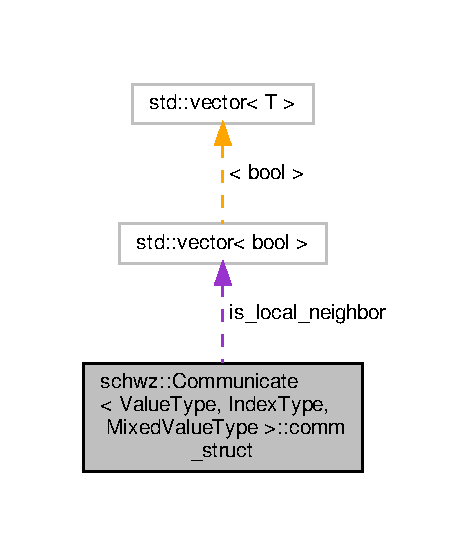
\includegraphics[width=226pt]{structschwz_1_1Communicate_1_1comm__struct__coll__graph}
\end{center}
\end{figure}
\subsection*{Public Attributes}
\begin{DoxyCompactItemize}
\item 
\mbox{\Hypertarget{structschwz_1_1Communicate_1_1comm__struct_aab657581d6c8ea5aba32f442edc4558f}\label{structschwz_1_1Communicate_1_1comm__struct_aab657581d6c8ea5aba32f442edc4558f}} 
int \hyperlink{structschwz_1_1Communicate_1_1comm__struct_aab657581d6c8ea5aba32f442edc4558f}{num\+\_\+neighbors\+\_\+in}
\begin{DoxyCompactList}\small\item\em The number of neighbors this subdomain has to receive data from. \end{DoxyCompactList}\item 
\mbox{\Hypertarget{structschwz_1_1Communicate_1_1comm__struct_a356e1582f7d5b0c4c8cba3eb11014b76}\label{structschwz_1_1Communicate_1_1comm__struct_a356e1582f7d5b0c4c8cba3eb11014b76}} 
int \hyperlink{structschwz_1_1Communicate_1_1comm__struct_a356e1582f7d5b0c4c8cba3eb11014b76}{num\+\_\+neighbors\+\_\+out}
\begin{DoxyCompactList}\small\item\em The number of neighbors this subdomain has to send data to. \end{DoxyCompactList}\item 
\mbox{\Hypertarget{structschwz_1_1Communicate_1_1comm__struct_a0dcb204149fb4f730e62255a84bc156a}\label{structschwz_1_1Communicate_1_1comm__struct_a0dcb204149fb4f730e62255a84bc156a}} 
std\+::shared\+\_\+ptr$<$ gko\+::\+Array$<$ Index\+Type $>$ $>$ \hyperlink{structschwz_1_1Communicate_1_1comm__struct_a0dcb204149fb4f730e62255a84bc156a}{neighbors\+\_\+in}
\begin{DoxyCompactList}\small\item\em The neighbors this subdomain has to receive data from. \end{DoxyCompactList}\item 
\mbox{\Hypertarget{structschwz_1_1Communicate_1_1comm__struct_a6ae39215a67e0a19131d0249e9fd2083}\label{structschwz_1_1Communicate_1_1comm__struct_a6ae39215a67e0a19131d0249e9fd2083}} 
std\+::shared\+\_\+ptr$<$ gko\+::\+Array$<$ Index\+Type $>$ $>$ \hyperlink{structschwz_1_1Communicate_1_1comm__struct_a6ae39215a67e0a19131d0249e9fd2083}{neighbors\+\_\+out}
\begin{DoxyCompactList}\small\item\em The neighbors this subdomain has to send data to. \end{DoxyCompactList}\item 
std\+::vector$<$ bool $>$ \hyperlink{structschwz_1_1Communicate_1_1comm__struct_ae36319cfa4fc09154135a2b121377d3b}{is\+\_\+local\+\_\+neighbor}
\begin{DoxyCompactList}\small\item\em The bool vector which is true if the neighbors of a subdomain are in one node. \end{DoxyCompactList}\item 
\mbox{\Hypertarget{structschwz_1_1Communicate_1_1comm__struct_a9d4febd22c050bd5bbeb0f122d74fdd0}\label{structschwz_1_1Communicate_1_1comm__struct_a9d4febd22c050bd5bbeb0f122d74fdd0}} 
int \hyperlink{structschwz_1_1Communicate_1_1comm__struct_a9d4febd22c050bd5bbeb0f122d74fdd0}{local\+\_\+num\+\_\+neighbors\+\_\+in}
\begin{DoxyCompactList}\small\item\em The number of neighbors this subdomain has to receive data from. \end{DoxyCompactList}\item 
\mbox{\Hypertarget{structschwz_1_1Communicate_1_1comm__struct_a8b211e456ef9f0947df8fad0e0428990}\label{structschwz_1_1Communicate_1_1comm__struct_a8b211e456ef9f0947df8fad0e0428990}} 
int \hyperlink{structschwz_1_1Communicate_1_1comm__struct_a8b211e456ef9f0947df8fad0e0428990}{local\+\_\+num\+\_\+neighbors\+\_\+out}
\begin{DoxyCompactList}\small\item\em The number of neighbors this subdomain has to send data to. \end{DoxyCompactList}\item 
\mbox{\Hypertarget{structschwz_1_1Communicate_1_1comm__struct_a4e43434348a60554ecfdbd448fa54f73}\label{structschwz_1_1Communicate_1_1comm__struct_a4e43434348a60554ecfdbd448fa54f73}} 
std\+::shared\+\_\+ptr$<$ gko\+::\+Array$<$ Index\+Type $>$ $>$ \hyperlink{structschwz_1_1Communicate_1_1comm__struct_a4e43434348a60554ecfdbd448fa54f73}{local\+\_\+neighbors\+\_\+in}
\begin{DoxyCompactList}\small\item\em The neighbors this subdomain has to receive data from. \end{DoxyCompactList}\item 
\mbox{\Hypertarget{structschwz_1_1Communicate_1_1comm__struct_a087b62605d0889090c6e67325dfa3fb0}\label{structschwz_1_1Communicate_1_1comm__struct_a087b62605d0889090c6e67325dfa3fb0}} 
std\+::shared\+\_\+ptr$<$ gko\+::\+Array$<$ Index\+Type $>$ $>$ \hyperlink{structschwz_1_1Communicate_1_1comm__struct_a087b62605d0889090c6e67325dfa3fb0}{local\+\_\+neighbors\+\_\+out}
\begin{DoxyCompactList}\small\item\em The neighbors this subdomain has to send data to. \end{DoxyCompactList}\item 
std\+::shared\+\_\+ptr$<$ gko\+::\+Array$<$ Index\+Type $\ast$ $>$ $>$ \hyperlink{structschwz_1_1Communicate_1_1comm__struct_a9186bd26e5826aa6ad88c863798593ac}{global\+\_\+put}
\begin{DoxyCompactList}\small\item\em The array containing the number of elements that each subdomain sends from the other. \end{DoxyCompactList}\item 
std\+::shared\+\_\+ptr$<$ gko\+::\+Array$<$ Index\+Type $\ast$ $>$ $>$ \hyperlink{structschwz_1_1Communicate_1_1comm__struct_ace7588b81dd2aa7a84e118df8137252b}{local\+\_\+put}
\begin{DoxyCompactList}\small\item\em The array containing the number of elements that each subdomain sends from the other. \end{DoxyCompactList}\item 
std\+::shared\+\_\+ptr$<$ gko\+::\+Array$<$ Index\+Type $\ast$ $>$ $>$ \hyperlink{structschwz_1_1Communicate_1_1comm__struct_a206d13b093699bf04bd1efb51c4290f2}{remote\+\_\+put}
\begin{DoxyCompactList}\small\item\em The array containing the number of elements that each subdomain sends from the other. \end{DoxyCompactList}\item 
std\+::shared\+\_\+ptr$<$ gko\+::\+Array$<$ Index\+Type $\ast$ $>$ $>$ \hyperlink{structschwz_1_1Communicate_1_1comm__struct_a4166e2bb75eeaf48ee39ca7cdc3adb01}{global\+\_\+get}
\begin{DoxyCompactList}\small\item\em The array containing the number of elements that each subdomain gets from the other. \end{DoxyCompactList}\item 
std\+::shared\+\_\+ptr$<$ gko\+::\+Array$<$ Index\+Type $\ast$ $>$ $>$ \hyperlink{structschwz_1_1Communicate_1_1comm__struct_ab4e91a457646f43106da98a58c332754}{local\+\_\+get}
\begin{DoxyCompactList}\small\item\em The array containing the number of elements that each subdomain gets from the other. \end{DoxyCompactList}\item 
std\+::shared\+\_\+ptr$<$ gko\+::\+Array$<$ Index\+Type $\ast$ $>$ $>$ \hyperlink{structschwz_1_1Communicate_1_1comm__struct_a70f57e5c0ab445089ca9d8bdc0fa3838}{remote\+\_\+get}
\begin{DoxyCompactList}\small\item\em The array containing the number of elements that each subdomain gets from the other. \end{DoxyCompactList}\item 
\mbox{\Hypertarget{structschwz_1_1Communicate_1_1comm__struct_a179dd67dc2d6ea4b71a6d5964cac18c6}\label{structschwz_1_1Communicate_1_1comm__struct_a179dd67dc2d6ea4b71a6d5964cac18c6}} 
std\+::shared\+\_\+ptr$<$ gko\+::\+Array$<$ Index\+Type $>$ $>$ \hyperlink{structschwz_1_1Communicate_1_1comm__struct_a179dd67dc2d6ea4b71a6d5964cac18c6}{window\+\_\+ids}
\begin{DoxyCompactList}\small\item\em The R\+D\+MA window ids. \end{DoxyCompactList}\item 
\mbox{\Hypertarget{structschwz_1_1Communicate_1_1comm__struct_a167c62a1a0cf2be8351e1ab65a264cf2}\label{structschwz_1_1Communicate_1_1comm__struct_a167c62a1a0cf2be8351e1ab65a264cf2}} 
std\+::shared\+\_\+ptr$<$ gko\+::\+Array$<$ Index\+Type $>$ $>$ \hyperlink{structschwz_1_1Communicate_1_1comm__struct_a167c62a1a0cf2be8351e1ab65a264cf2}{windows\+\_\+from}
\begin{DoxyCompactList}\small\item\em The R\+D\+MA window ids to receive data from. \end{DoxyCompactList}\item 
\mbox{\Hypertarget{structschwz_1_1Communicate_1_1comm__struct_aef866f16ced557ba1496cffaf7c2473e}\label{structschwz_1_1Communicate_1_1comm__struct_aef866f16ced557ba1496cffaf7c2473e}} 
std\+::shared\+\_\+ptr$<$ gko\+::\+Array$<$ Index\+Type $>$ $>$ \hyperlink{structschwz_1_1Communicate_1_1comm__struct_aef866f16ced557ba1496cffaf7c2473e}{windows\+\_\+to}
\begin{DoxyCompactList}\small\item\em The R\+D\+MA window ids to send data to. \end{DoxyCompactList}\item 
\mbox{\Hypertarget{structschwz_1_1Communicate_1_1comm__struct_a9f135d4c33838027f8ed64a3ee18d42f}\label{structschwz_1_1Communicate_1_1comm__struct_a9f135d4c33838027f8ed64a3ee18d42f}} 
std\+::shared\+\_\+ptr$<$ gko\+::\+Array$<$ M\+P\+I\+\_\+\+Request $>$ $>$ \hyperlink{structschwz_1_1Communicate_1_1comm__struct_a9f135d4c33838027f8ed64a3ee18d42f}{put\+\_\+request}
\begin{DoxyCompactList}\small\item\em The put request array. \end{DoxyCompactList}\item 
\mbox{\Hypertarget{structschwz_1_1Communicate_1_1comm__struct_a91cc6e7d906fbb693e4dff2dee609c94}\label{structschwz_1_1Communicate_1_1comm__struct_a91cc6e7d906fbb693e4dff2dee609c94}} 
std\+::shared\+\_\+ptr$<$ gko\+::\+Array$<$ M\+P\+I\+\_\+\+Request $>$ $>$ \hyperlink{structschwz_1_1Communicate_1_1comm__struct_a91cc6e7d906fbb693e4dff2dee609c94}{get\+\_\+request}
\begin{DoxyCompactList}\small\item\em The get request array. \end{DoxyCompactList}\item 
\mbox{\Hypertarget{structschwz_1_1Communicate_1_1comm__struct_afc441e718856c45bd3cc462780886ca8}\label{structschwz_1_1Communicate_1_1comm__struct_afc441e718856c45bd3cc462780886ca8}} 
std\+::shared\+\_\+ptr$<$ gko\+::matrix\+::\+Dense$<$ Value\+Type $>$ $>$ \hyperlink{structschwz_1_1Communicate_1_1comm__struct_afc441e718856c45bd3cc462780886ca8}{send\+\_\+buffer}
\begin{DoxyCompactList}\small\item\em The send buffer used for the actual communication for both one-\/sided and two-\/sided. \end{DoxyCompactList}\item 
\mbox{\Hypertarget{structschwz_1_1Communicate_1_1comm__struct_a357d96eeeb734a275f78782e7e6542a8}\label{structschwz_1_1Communicate_1_1comm__struct_a357d96eeeb734a275f78782e7e6542a8}} 
std\+::shared\+\_\+ptr$<$ gko\+::matrix\+::\+Dense$<$ Mixed\+Value\+Type $>$ $>$ \hyperlink{structschwz_1_1Communicate_1_1comm__struct_a357d96eeeb734a275f78782e7e6542a8}{mixedt\+\_\+send\+\_\+buffer}
\begin{DoxyCompactList}\small\item\em The mixed send buffer used for the actual communication for both one-\/sided and two-\/sided. \end{DoxyCompactList}\item 
\mbox{\Hypertarget{structschwz_1_1Communicate_1_1comm__struct_a7b02126d598b9054b9adf0ebc9b3138c}\label{structschwz_1_1Communicate_1_1comm__struct_a7b02126d598b9054b9adf0ebc9b3138c}} 
std\+::shared\+\_\+ptr$<$ gko\+::matrix\+::\+Dense$<$ Value\+Type $>$ $>$ \hyperlink{structschwz_1_1Communicate_1_1comm__struct_a7b02126d598b9054b9adf0ebc9b3138c}{recv\+\_\+buffer}
\begin{DoxyCompactList}\small\item\em The recv buffer used for the actual communication for both one-\/sided and two-\/sided. \end{DoxyCompactList}\item 
\mbox{\Hypertarget{structschwz_1_1Communicate_1_1comm__struct_a93ca78673122ad09e24bebd0b1ec9750}\label{structschwz_1_1Communicate_1_1comm__struct_a93ca78673122ad09e24bebd0b1ec9750}} 
std\+::shared\+\_\+ptr$<$ gko\+::matrix\+::\+Dense$<$ Mixed\+Value\+Type $>$ $>$ \hyperlink{structschwz_1_1Communicate_1_1comm__struct_a93ca78673122ad09e24bebd0b1ec9750}{mixedt\+\_\+recv\+\_\+buffer}
\begin{DoxyCompactList}\small\item\em The mixed precision recv buffer used for the actual communication for both one-\/sided and two-\/sided. \end{DoxyCompactList}\item 
\mbox{\Hypertarget{structschwz_1_1Communicate_1_1comm__struct_aa9d510fb291e896fa14fe3e0f00f0454}\label{structschwz_1_1Communicate_1_1comm__struct_aa9d510fb291e896fa14fe3e0f00f0454}} 
std\+::shared\+\_\+ptr$<$ gko\+::\+Array$<$ Index\+Type $>$ $>$ \hyperlink{structschwz_1_1Communicate_1_1comm__struct_aa9d510fb291e896fa14fe3e0f00f0454}{get\+\_\+displacements}
\begin{DoxyCompactList}\small\item\em The displacements for the receiving of the buffer. \end{DoxyCompactList}\item 
\mbox{\Hypertarget{structschwz_1_1Communicate_1_1comm__struct_abb06062ad6fddb9d0399625f4d799d08}\label{structschwz_1_1Communicate_1_1comm__struct_abb06062ad6fddb9d0399625f4d799d08}} 
std\+::shared\+\_\+ptr$<$ gko\+::\+Array$<$ Index\+Type $>$ $>$ \hyperlink{structschwz_1_1Communicate_1_1comm__struct_abb06062ad6fddb9d0399625f4d799d08}{put\+\_\+displacements}
\begin{DoxyCompactList}\small\item\em The displacements for the sending of the buffer. \end{DoxyCompactList}\item 
\mbox{\Hypertarget{structschwz_1_1Communicate_1_1comm__struct_a6257c71a7ebf30ecfc390059ceef0e1f}\label{structschwz_1_1Communicate_1_1comm__struct_a6257c71a7ebf30ecfc390059ceef0e1f}} 
M\+P\+I\+\_\+\+Win \hyperlink{structschwz_1_1Communicate_1_1comm__struct_a6257c71a7ebf30ecfc390059ceef0e1f}{window\+\_\+recv\+\_\+buffer}
\begin{DoxyCompactList}\small\item\em The R\+D\+MA window for the recv buffer. \end{DoxyCompactList}\item 
\mbox{\Hypertarget{structschwz_1_1Communicate_1_1comm__struct_af2c5d4bfea8073b2c885eec175b92416}\label{structschwz_1_1Communicate_1_1comm__struct_af2c5d4bfea8073b2c885eec175b92416}} 
M\+P\+I\+\_\+\+Win \hyperlink{structschwz_1_1Communicate_1_1comm__struct_af2c5d4bfea8073b2c885eec175b92416}{window\+\_\+send\+\_\+buffer}
\begin{DoxyCompactList}\small\item\em The R\+D\+MA window for the send buffer. \end{DoxyCompactList}\item 
\mbox{\Hypertarget{structschwz_1_1Communicate_1_1comm__struct_a5da0c24baf9d9955d764fe4b3274a982}\label{structschwz_1_1Communicate_1_1comm__struct_a5da0c24baf9d9955d764fe4b3274a982}} 
M\+P\+I\+\_\+\+Win \hyperlink{structschwz_1_1Communicate_1_1comm__struct_a5da0c24baf9d9955d764fe4b3274a982}{window\+\_\+x}
\begin{DoxyCompactList}\small\item\em The R\+D\+MA window for the solution vector. \end{DoxyCompactList}\end{DoxyCompactItemize}


\subsection{Detailed Description}
\subsubsection*{template$<$typename Value\+Type, typename Index\+Type, typename Mixed\+Value\+Type$>$\newline
struct schwz\+::\+Communicate$<$ Value\+Type, Index\+Type, Mixed\+Value\+Type $>$\+::comm\+\_\+struct}

The communication struct used to store the communication data. 

\subsection{Member Data Documentation}
\mbox{\Hypertarget{structschwz_1_1Communicate_1_1comm__struct_a4166e2bb75eeaf48ee39ca7cdc3adb01}\label{structschwz_1_1Communicate_1_1comm__struct_a4166e2bb75eeaf48ee39ca7cdc3adb01}} 
\index{schwz\+::\+Communicate\+::comm\+\_\+struct@{schwz\+::\+Communicate\+::comm\+\_\+struct}!global\+\_\+get@{global\+\_\+get}}
\index{global\+\_\+get@{global\+\_\+get}!schwz\+::\+Communicate\+::comm\+\_\+struct@{schwz\+::\+Communicate\+::comm\+\_\+struct}}
\subsubsection{\texorpdfstring{global\+\_\+get}{global\_get}}
{\footnotesize\ttfamily template$<$typename Value\+Type , typename Index\+Type , typename Mixed\+Value\+Type $>$ \\
std\+::shared\+\_\+ptr$<$gko\+::\+Array$<$Index\+Type $\ast$$>$ $>$ \hyperlink{classschwz_1_1Communicate}{schwz\+::\+Communicate}$<$ Value\+Type, Index\+Type, Mixed\+Value\+Type $>$\+::comm\+\_\+struct\+::global\+\_\+get}



The array containing the number of elements that each subdomain gets from the other. 

For example. global\+\_\+get\mbox{[}p\mbox{]}\mbox{[}0\mbox{]} contains the overall number of elements to be received to subdomain p and global\+\_\+put\mbox{[}p\mbox{]}\mbox{[}i\mbox{]} contains the index of the solution vector to be received from subdomain p. 

Referenced by schwz\+::\+Schwarz\+Base$<$ Value\+Type, Index\+Type, Mixed\+Value\+Type $>$\+::initialize(), schwz\+::\+Solver\+R\+A\+S$<$ Value\+Type, Index\+Type, Mixed\+Value\+Type $>$\+::setup\+\_\+comm\+\_\+buffers(), and schwz\+::\+Solver\+R\+A\+S$<$ Value\+Type, Index\+Type, Mixed\+Value\+Type $>$\+::setup\+\_\+windows().

\mbox{\Hypertarget{structschwz_1_1Communicate_1_1comm__struct_a9186bd26e5826aa6ad88c863798593ac}\label{structschwz_1_1Communicate_1_1comm__struct_a9186bd26e5826aa6ad88c863798593ac}} 
\index{schwz\+::\+Communicate\+::comm\+\_\+struct@{schwz\+::\+Communicate\+::comm\+\_\+struct}!global\+\_\+put@{global\+\_\+put}}
\index{global\+\_\+put@{global\+\_\+put}!schwz\+::\+Communicate\+::comm\+\_\+struct@{schwz\+::\+Communicate\+::comm\+\_\+struct}}
\subsubsection{\texorpdfstring{global\+\_\+put}{global\_put}}
{\footnotesize\ttfamily template$<$typename Value\+Type , typename Index\+Type , typename Mixed\+Value\+Type $>$ \\
std\+::shared\+\_\+ptr$<$gko\+::\+Array$<$Index\+Type $\ast$$>$ $>$ \hyperlink{classschwz_1_1Communicate}{schwz\+::\+Communicate}$<$ Value\+Type, Index\+Type, Mixed\+Value\+Type $>$\+::comm\+\_\+struct\+::global\+\_\+put}



The array containing the number of elements that each subdomain sends from the other. 

For example. global\+\_\+put\mbox{[}p\mbox{]}\mbox{[}0\mbox{]} contains the overall number of elements to be sent to subdomain p and global\+\_\+put\mbox{[}p\mbox{]}\mbox{[}i\mbox{]} contains the index of the solution vector to be sent to subdomain p. 

Referenced by schwz\+::\+Schwarz\+Base$<$ Value\+Type, Index\+Type, Mixed\+Value\+Type $>$\+::initialize(), schwz\+::\+Solver\+R\+A\+S$<$ Value\+Type, Index\+Type, Mixed\+Value\+Type $>$\+::setup\+\_\+comm\+\_\+buffers(), and schwz\+::\+Solver\+R\+A\+S$<$ Value\+Type, Index\+Type, Mixed\+Value\+Type $>$\+::setup\+\_\+windows().

\mbox{\Hypertarget{structschwz_1_1Communicate_1_1comm__struct_ae36319cfa4fc09154135a2b121377d3b}\label{structschwz_1_1Communicate_1_1comm__struct_ae36319cfa4fc09154135a2b121377d3b}} 
\index{schwz\+::\+Communicate\+::comm\+\_\+struct@{schwz\+::\+Communicate\+::comm\+\_\+struct}!is\+\_\+local\+\_\+neighbor@{is\+\_\+local\+\_\+neighbor}}
\index{is\+\_\+local\+\_\+neighbor@{is\+\_\+local\+\_\+neighbor}!schwz\+::\+Communicate\+::comm\+\_\+struct@{schwz\+::\+Communicate\+::comm\+\_\+struct}}
\subsubsection{\texorpdfstring{is\+\_\+local\+\_\+neighbor}{is\_local\_neighbor}}
{\footnotesize\ttfamily template$<$typename Value\+Type , typename Index\+Type , typename Mixed\+Value\+Type $>$ \\
std\+::vector$<$bool$>$ \hyperlink{classschwz_1_1Communicate}{schwz\+::\+Communicate}$<$ Value\+Type, Index\+Type, Mixed\+Value\+Type $>$\+::comm\+\_\+struct\+::is\+\_\+local\+\_\+neighbor}



The bool vector which is true if the neighbors of a subdomain are in one node. 



Referenced by schwz\+::\+Schwarz\+Base$<$ Value\+Type, Index\+Type, Mixed\+Value\+Type $>$\+::initialize(), schwz\+::\+Solver\+R\+A\+S$<$ Value\+Type, Index\+Type, Mixed\+Value\+Type $>$\+::setup\+\_\+comm\+\_\+buffers(), and schwz\+::\+Solver\+R\+A\+S$<$ Value\+Type, Index\+Type, Mixed\+Value\+Type $>$\+::setup\+\_\+windows().

\mbox{\Hypertarget{structschwz_1_1Communicate_1_1comm__struct_ab4e91a457646f43106da98a58c332754}\label{structschwz_1_1Communicate_1_1comm__struct_ab4e91a457646f43106da98a58c332754}} 
\index{schwz\+::\+Communicate\+::comm\+\_\+struct@{schwz\+::\+Communicate\+::comm\+\_\+struct}!local\+\_\+get@{local\+\_\+get}}
\index{local\+\_\+get@{local\+\_\+get}!schwz\+::\+Communicate\+::comm\+\_\+struct@{schwz\+::\+Communicate\+::comm\+\_\+struct}}
\subsubsection{\texorpdfstring{local\+\_\+get}{local\_get}}
{\footnotesize\ttfamily template$<$typename Value\+Type , typename Index\+Type , typename Mixed\+Value\+Type $>$ \\
std\+::shared\+\_\+ptr$<$gko\+::\+Array$<$Index\+Type $\ast$$>$ $>$ \hyperlink{classschwz_1_1Communicate}{schwz\+::\+Communicate}$<$ Value\+Type, Index\+Type, Mixed\+Value\+Type $>$\+::comm\+\_\+struct\+::local\+\_\+get}



The array containing the number of elements that each subdomain gets from the other. 

For example. global\+\_\+get\mbox{[}p\mbox{]}\mbox{[}0\mbox{]} contains the overall number of elements to be received to subdomain p and global\+\_\+put\mbox{[}p\mbox{]}\mbox{[}i\mbox{]} contains the index of the solution vector to be received from subdomain p. 

Referenced by schwz\+::\+Solver\+R\+A\+S$<$ Value\+Type, Index\+Type, Mixed\+Value\+Type $>$\+::setup\+\_\+comm\+\_\+buffers(), and schwz\+::\+Solver\+R\+A\+S$<$ Value\+Type, Index\+Type, Mixed\+Value\+Type $>$\+::setup\+\_\+windows().

\mbox{\Hypertarget{structschwz_1_1Communicate_1_1comm__struct_ace7588b81dd2aa7a84e118df8137252b}\label{structschwz_1_1Communicate_1_1comm__struct_ace7588b81dd2aa7a84e118df8137252b}} 
\index{schwz\+::\+Communicate\+::comm\+\_\+struct@{schwz\+::\+Communicate\+::comm\+\_\+struct}!local\+\_\+put@{local\+\_\+put}}
\index{local\+\_\+put@{local\+\_\+put}!schwz\+::\+Communicate\+::comm\+\_\+struct@{schwz\+::\+Communicate\+::comm\+\_\+struct}}
\subsubsection{\texorpdfstring{local\+\_\+put}{local\_put}}
{\footnotesize\ttfamily template$<$typename Value\+Type , typename Index\+Type , typename Mixed\+Value\+Type $>$ \\
std\+::shared\+\_\+ptr$<$gko\+::\+Array$<$Index\+Type $\ast$$>$ $>$ \hyperlink{classschwz_1_1Communicate}{schwz\+::\+Communicate}$<$ Value\+Type, Index\+Type, Mixed\+Value\+Type $>$\+::comm\+\_\+struct\+::local\+\_\+put}



The array containing the number of elements that each subdomain sends from the other. 

For example. global\+\_\+put\mbox{[}p\mbox{]}\mbox{[}0\mbox{]} contains the overall number of elements to be sent to subdomain p and global\+\_\+put\mbox{[}p\mbox{]}\mbox{[}i\mbox{]} contains the index of the solution vector to be sent to subdomain p. 

Referenced by schwz\+::\+Solver\+R\+A\+S$<$ Value\+Type, Index\+Type, Mixed\+Value\+Type $>$\+::setup\+\_\+comm\+\_\+buffers(), and schwz\+::\+Solver\+R\+A\+S$<$ Value\+Type, Index\+Type, Mixed\+Value\+Type $>$\+::setup\+\_\+windows().

\mbox{\Hypertarget{structschwz_1_1Communicate_1_1comm__struct_a70f57e5c0ab445089ca9d8bdc0fa3838}\label{structschwz_1_1Communicate_1_1comm__struct_a70f57e5c0ab445089ca9d8bdc0fa3838}} 
\index{schwz\+::\+Communicate\+::comm\+\_\+struct@{schwz\+::\+Communicate\+::comm\+\_\+struct}!remote\+\_\+get@{remote\+\_\+get}}
\index{remote\+\_\+get@{remote\+\_\+get}!schwz\+::\+Communicate\+::comm\+\_\+struct@{schwz\+::\+Communicate\+::comm\+\_\+struct}}
\subsubsection{\texorpdfstring{remote\+\_\+get}{remote\_get}}
{\footnotesize\ttfamily template$<$typename Value\+Type , typename Index\+Type , typename Mixed\+Value\+Type $>$ \\
std\+::shared\+\_\+ptr$<$gko\+::\+Array$<$Index\+Type $\ast$$>$ $>$ \hyperlink{classschwz_1_1Communicate}{schwz\+::\+Communicate}$<$ Value\+Type, Index\+Type, Mixed\+Value\+Type $>$\+::comm\+\_\+struct\+::remote\+\_\+get}



The array containing the number of elements that each subdomain gets from the other. 

For example. global\+\_\+get\mbox{[}p\mbox{]}\mbox{[}0\mbox{]} contains the overall number of elements to be received to subdomain p and global\+\_\+put\mbox{[}p\mbox{]}\mbox{[}i\mbox{]} contains the index of the solution vector to be received from subdomain p. 

Referenced by schwz\+::\+Solver\+R\+A\+S$<$ Value\+Type, Index\+Type, Mixed\+Value\+Type $>$\+::setup\+\_\+comm\+\_\+buffers(), and schwz\+::\+Solver\+R\+A\+S$<$ Value\+Type, Index\+Type, Mixed\+Value\+Type $>$\+::setup\+\_\+windows().

\mbox{\Hypertarget{structschwz_1_1Communicate_1_1comm__struct_a206d13b093699bf04bd1efb51c4290f2}\label{structschwz_1_1Communicate_1_1comm__struct_a206d13b093699bf04bd1efb51c4290f2}} 
\index{schwz\+::\+Communicate\+::comm\+\_\+struct@{schwz\+::\+Communicate\+::comm\+\_\+struct}!remote\+\_\+put@{remote\+\_\+put}}
\index{remote\+\_\+put@{remote\+\_\+put}!schwz\+::\+Communicate\+::comm\+\_\+struct@{schwz\+::\+Communicate\+::comm\+\_\+struct}}
\subsubsection{\texorpdfstring{remote\+\_\+put}{remote\_put}}
{\footnotesize\ttfamily template$<$typename Value\+Type , typename Index\+Type , typename Mixed\+Value\+Type $>$ \\
std\+::shared\+\_\+ptr$<$gko\+::\+Array$<$Index\+Type $\ast$$>$ $>$ \hyperlink{classschwz_1_1Communicate}{schwz\+::\+Communicate}$<$ Value\+Type, Index\+Type, Mixed\+Value\+Type $>$\+::comm\+\_\+struct\+::remote\+\_\+put}



The array containing the number of elements that each subdomain sends from the other. 

For example. global\+\_\+put\mbox{[}p\mbox{]}\mbox{[}0\mbox{]} contains the overall number of elements to be sent to subdomain p and global\+\_\+put\mbox{[}p\mbox{]}\mbox{[}i\mbox{]} contains the index of the solution vector to be sent to subdomain p. 

Referenced by schwz\+::\+Solver\+R\+A\+S$<$ Value\+Type, Index\+Type, Mixed\+Value\+Type $>$\+::setup\+\_\+comm\+\_\+buffers(), and schwz\+::\+Solver\+R\+A\+S$<$ Value\+Type, Index\+Type, Mixed\+Value\+Type $>$\+::setup\+\_\+windows().



The documentation for this struct was generated from the following file\+:\begin{DoxyCompactItemize}
\item 
communicate.\+hpp (ebc6847)\end{DoxyCompactItemize}

\hypertarget{classschwz_1_1Communicate}{}\section{schwz\+:\+:Communicate$<$ Value\+Type, Index\+Type, Mixed\+Value\+Type $>$ Class Template Reference}
\label{classschwz_1_1Communicate}\index{schwz\+::\+Communicate$<$ Value\+Type, Index\+Type, Mixed\+Value\+Type $>$@{schwz\+::\+Communicate$<$ Value\+Type, Index\+Type, Mixed\+Value\+Type $>$}}


The communication class that provides the methods for the communication between the subdomains.  




{\ttfamily \#include $<$communicate.\+hpp$>$}



Collaboration diagram for schwz\+:\+:Communicate$<$ Value\+Type, Index\+Type, Mixed\+Value\+Type $>$\+:
\nopagebreak
\begin{figure}[H]
\begin{center}
\leavevmode
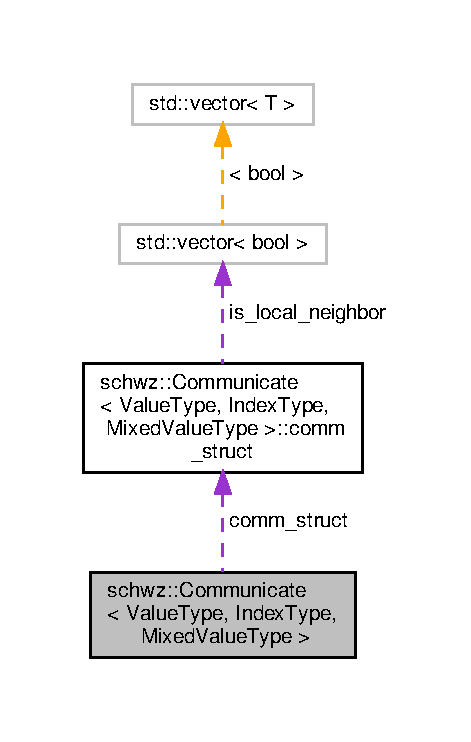
\includegraphics[width=226pt]{classschwz_1_1Communicate__coll__graph}
\end{center}
\end{figure}
\subsection*{Classes}
\begin{DoxyCompactItemize}
\item 
struct \hyperlink{structschwz_1_1Communicate_1_1comm__struct}{comm\+\_\+struct}
\begin{DoxyCompactList}\small\item\em The communication struct used to store the communication data. \end{DoxyCompactList}\end{DoxyCompactItemize}
\subsection*{Public Member Functions}
\begin{DoxyCompactItemize}
\item 
\mbox{\Hypertarget{classschwz_1_1Communicate_a76b0d6b0571107ab2cd58e309902a666}\label{classschwz_1_1Communicate_a76b0d6b0571107ab2cd58e309902a666}} 
virtual void \hyperlink{classschwz_1_1Communicate_a76b0d6b0571107ab2cd58e309902a666}{setup\+\_\+comm\+\_\+buffers} ()=0
\begin{DoxyCompactList}\small\item\em Sets up the communication buffers needed for the boundary exchange. \end{DoxyCompactList}\item 
virtual void \hyperlink{classschwz_1_1Communicate_a13190372f3a6193f92226d08e822fde7}{setup\+\_\+windows} (const \hyperlink{structschwz_1_1Settings}{Settings} \&settings, const \hyperlink{structschwz_1_1Metadata}{Metadata}$<$ Value\+Type, Index\+Type $>$ \&metadata, std\+::shared\+\_\+ptr$<$ gko\+::matrix\+::\+Dense$<$ Value\+Type $>$$>$ \&main\+\_\+buffer)=0
\begin{DoxyCompactList}\small\item\em Sets up the windows needed for the asynchronous communication. \end{DoxyCompactList}\item 
virtual void \hyperlink{classschwz_1_1Communicate_a41794ecd95f7f7e590ae27bb6ca6e6e1}{exchange\+\_\+boundary} (const \hyperlink{structschwz_1_1Settings}{Settings} \&settings, const \hyperlink{structschwz_1_1Metadata}{Metadata}$<$ Value\+Type, Index\+Type $>$ \&metadata, std\+::shared\+\_\+ptr$<$ gko\+::matrix\+::\+Dense$<$ Value\+Type $>$$>$ \&global\+\_\+solution)=0
\begin{DoxyCompactList}\small\item\em Exchanges the elements of the solution vector. \end{DoxyCompactList}\item 
void \hyperlink{classschwz_1_1Communicate_a8c1ed0c5f86c458038b4062f57337d44}{local\+\_\+to\+\_\+global\+\_\+vector} (const \hyperlink{structschwz_1_1Settings}{Settings} \&settings, const \hyperlink{structschwz_1_1Metadata}{Metadata}$<$ Value\+Type, Index\+Type $>$ \&metadata, const std\+::shared\+\_\+ptr$<$ gko\+::matrix\+::\+Dense$<$ Value\+Type $>$$>$ \&local\+\_\+vector, std\+::shared\+\_\+ptr$<$ gko\+::matrix\+::\+Dense$<$ Value\+Type $>$$>$ \&global\+\_\+vector)
\begin{DoxyCompactList}\small\item\em Transforms data from a local vector to a global vector. \end{DoxyCompactList}\item 
virtual void \hyperlink{classschwz_1_1Communicate_a371fb6c61c0bd9b619bbe7e154d18696}{update\+\_\+boundary} (const \hyperlink{structschwz_1_1Settings}{Settings} \&settings, const \hyperlink{structschwz_1_1Metadata}{Metadata}$<$ Value\+Type, Index\+Type $>$ \&metadata, std\+::shared\+\_\+ptr$<$ gko\+::matrix\+::\+Dense$<$ Value\+Type $>$$>$ \&local\+\_\+solution, const std\+::shared\+\_\+ptr$<$ gko\+::matrix\+::\+Dense$<$ Value\+Type $>$$>$ \&local\+\_\+rhs, const std\+::shared\+\_\+ptr$<$ gko\+::matrix\+::\+Dense$<$ Value\+Type $>$$>$ \&global\+\_\+solution, const std\+::shared\+\_\+ptr$<$ gko\+::matrix\+::\+Csr$<$ Value\+Type, Index\+Type $>$$>$ \&interface\+\_\+matrix)=0
\begin{DoxyCompactList}\small\item\em Update the values into local vector from obtained from the neighboring sub-\/domains using the interface matrix. \end{DoxyCompactList}\item 
\mbox{\Hypertarget{classschwz_1_1Communicate_ac01c45763b2945b0c361b49c7305b142}\label{classschwz_1_1Communicate_ac01c45763b2945b0c361b49c7305b142}} 
void \hyperlink{classschwz_1_1Communicate_ac01c45763b2945b0c361b49c7305b142}{clear} (\hyperlink{structschwz_1_1Settings}{Settings} \&settings)
\begin{DoxyCompactList}\small\item\em Clears the data. \end{DoxyCompactList}\end{DoxyCompactItemize}
\subsection*{Public Attributes}
\begin{DoxyCompactItemize}
\item 
\mbox{\Hypertarget{classschwz_1_1Communicate_ab9c6c68bfa363819322189192ca014aa}\label{classschwz_1_1Communicate_ab9c6c68bfa363819322189192ca014aa}} 
\hyperlink{structschwz_1_1Communicate_1_1comm__struct}{comm\+\_\+struct} {\bfseries comm\+\_\+struct}
\end{DoxyCompactItemize}
\subsection*{Friends}
\begin{DoxyCompactItemize}
\item 
\mbox{\Hypertarget{classschwz_1_1Communicate_a7044b349fe5363eeace2d1a56b38f650}\label{classschwz_1_1Communicate_a7044b349fe5363eeace2d1a56b38f650}} 
class {\bfseries Initialize$<$ Value\+Type, Index\+Type $>$}
\end{DoxyCompactItemize}


\subsection{Detailed Description}
\subsubsection*{template$<$typename Value\+Type, typename Index\+Type, typename Mixed\+Value\+Type$>$\newline
class schwz\+::\+Communicate$<$ Value\+Type, Index\+Type, Mixed\+Value\+Type $>$}

The communication class that provides the methods for the communication between the subdomains. 


\begin{DoxyTemplParams}{Template Parameters}
{\em Value\+Type} & The type of the floating point values. \\
\hline
{\em Index\+Type} & The type of the index type values.\\
\hline
\end{DoxyTemplParams}
\hyperlink{group__comm}{Communicate} 

\subsection{Member Function Documentation}
\mbox{\Hypertarget{classschwz_1_1Communicate_a41794ecd95f7f7e590ae27bb6ca6e6e1}\label{classschwz_1_1Communicate_a41794ecd95f7f7e590ae27bb6ca6e6e1}} 
\index{schwz\+::\+Communicate@{schwz\+::\+Communicate}!exchange\+\_\+boundary@{exchange\+\_\+boundary}}
\index{exchange\+\_\+boundary@{exchange\+\_\+boundary}!schwz\+::\+Communicate@{schwz\+::\+Communicate}}
\subsubsection{\texorpdfstring{exchange\+\_\+boundary()}{exchange\_boundary()}}
{\footnotesize\ttfamily template$<$typename Value\+Type , typename Index\+Type , typename Mixed\+Value\+Type $>$ \\
void \hyperlink{classschwz_1_1Communicate}{schwz\+::\+Communicate}$<$ Value\+Type, Index\+Type, Mixed\+Value\+Type $>$\+::exchange\+\_\+boundary (\begin{DoxyParamCaption}\item[{const \hyperlink{structschwz_1_1Settings}{Settings} \&}]{settings,  }\item[{const \hyperlink{structschwz_1_1Metadata}{Metadata}$<$ Value\+Type, Index\+Type $>$ \&}]{metadata,  }\item[{std\+::shared\+\_\+ptr$<$ gko\+::matrix\+::\+Dense$<$ Value\+Type $>$$>$ \&}]{global\+\_\+solution }\end{DoxyParamCaption})\hspace{0.3cm}{\ttfamily [pure virtual]}}



Exchanges the elements of the solution vector. 


\begin{DoxyParams}{Parameters}
{\em settings} & The settings struct. \\
\hline
{\em metadata} & The metadata struct. \\
\hline
{\em global\+\_\+solution} & The solution vector being exchanged between the subdomains. \\
\hline
\end{DoxyParams}


Implemented in \hyperlink{classschwz_1_1SolverRAS_ab8983c89cdc7b45d15f9f4bf276e9753}{schwz\+::\+Solver\+R\+A\+S$<$ Value\+Type, Index\+Type, Mixed\+Value\+Type $>$}.



Referenced by schwz\+::\+Schwarz\+Base$<$ Value\+Type, Index\+Type, Mixed\+Value\+Type $>$\+::run().

\mbox{\Hypertarget{classschwz_1_1Communicate_a8c1ed0c5f86c458038b4062f57337d44}\label{classschwz_1_1Communicate_a8c1ed0c5f86c458038b4062f57337d44}} 
\index{schwz\+::\+Communicate@{schwz\+::\+Communicate}!local\+\_\+to\+\_\+global\+\_\+vector@{local\+\_\+to\+\_\+global\+\_\+vector}}
\index{local\+\_\+to\+\_\+global\+\_\+vector@{local\+\_\+to\+\_\+global\+\_\+vector}!schwz\+::\+Communicate@{schwz\+::\+Communicate}}
\subsubsection{\texorpdfstring{local\+\_\+to\+\_\+global\+\_\+vector()}{local\_to\_global\_vector()}}
{\footnotesize\ttfamily template$<$typename Value\+Type , typename Index\+Type , typename Mixed\+Value\+Type $>$ \\
void \hyperlink{classschwz_1_1Communicate}{schwz\+::\+Communicate}$<$ Value\+Type, Index\+Type, Mixed\+Value\+Type $>$\+::local\+\_\+to\+\_\+global\+\_\+vector (\begin{DoxyParamCaption}\item[{const \hyperlink{structschwz_1_1Settings}{Settings} \&}]{settings,  }\item[{const \hyperlink{structschwz_1_1Metadata}{Metadata}$<$ Value\+Type, Index\+Type $>$ \&}]{metadata,  }\item[{const std\+::shared\+\_\+ptr$<$ gko\+::matrix\+::\+Dense$<$ Value\+Type $>$$>$ \&}]{local\+\_\+vector,  }\item[{std\+::shared\+\_\+ptr$<$ gko\+::matrix\+::\+Dense$<$ Value\+Type $>$$>$ \&}]{global\+\_\+vector }\end{DoxyParamCaption})}



Transforms data from a local vector to a global vector. 


\begin{DoxyParams}{Parameters}
{\em settings} & The settings struct. \\
\hline
{\em metadata} & The metadata struct. \\
\hline
{\em local\+\_\+vector} & The local vector in question. \\
\hline
{\em global\+\_\+vector} & The global vector in question. \\
\hline
\end{DoxyParams}


Referenced by schwz\+::\+Schwarz\+Base$<$ Value\+Type, Index\+Type, Mixed\+Value\+Type $>$\+::run().

\mbox{\Hypertarget{classschwz_1_1Communicate_a13190372f3a6193f92226d08e822fde7}\label{classschwz_1_1Communicate_a13190372f3a6193f92226d08e822fde7}} 
\index{schwz\+::\+Communicate@{schwz\+::\+Communicate}!setup\+\_\+windows@{setup\+\_\+windows}}
\index{setup\+\_\+windows@{setup\+\_\+windows}!schwz\+::\+Communicate@{schwz\+::\+Communicate}}
\subsubsection{\texorpdfstring{setup\+\_\+windows()}{setup\_windows()}}
{\footnotesize\ttfamily template$<$typename Value\+Type , typename Index\+Type , typename Mixed\+Value\+Type $>$ \\
void \hyperlink{classschwz_1_1Communicate}{schwz\+::\+Communicate}$<$ Value\+Type, Index\+Type, Mixed\+Value\+Type $>$\+::setup\+\_\+windows (\begin{DoxyParamCaption}\item[{const \hyperlink{structschwz_1_1Settings}{Settings} \&}]{settings,  }\item[{const \hyperlink{structschwz_1_1Metadata}{Metadata}$<$ Value\+Type, Index\+Type $>$ \&}]{metadata,  }\item[{std\+::shared\+\_\+ptr$<$ gko\+::matrix\+::\+Dense$<$ Value\+Type $>$$>$ \&}]{main\+\_\+buffer }\end{DoxyParamCaption})\hspace{0.3cm}{\ttfamily [pure virtual]}}



Sets up the windows needed for the asynchronous communication. 


\begin{DoxyParams}{Parameters}
{\em settings} & The settings struct. \\
\hline
{\em metadata} & The metadata struct. \\
\hline
{\em main\+\_\+buffer} & The main buffer being exchanged between the subdomains. \\
\hline
\end{DoxyParams}


Implemented in \hyperlink{classschwz_1_1SolverRAS_adc313354f7ae256d375316516d0f655e}{schwz\+::\+Solver\+R\+A\+S$<$ Value\+Type, Index\+Type, Mixed\+Value\+Type $>$}.



Referenced by schwz\+::\+Schwarz\+Base$<$ Value\+Type, Index\+Type, Mixed\+Value\+Type $>$\+::run().

\mbox{\Hypertarget{classschwz_1_1Communicate_a371fb6c61c0bd9b619bbe7e154d18696}\label{classschwz_1_1Communicate_a371fb6c61c0bd9b619bbe7e154d18696}} 
\index{schwz\+::\+Communicate@{schwz\+::\+Communicate}!update\+\_\+boundary@{update\+\_\+boundary}}
\index{update\+\_\+boundary@{update\+\_\+boundary}!schwz\+::\+Communicate@{schwz\+::\+Communicate}}
\subsubsection{\texorpdfstring{update\+\_\+boundary()}{update\_boundary()}}
{\footnotesize\ttfamily template$<$typename Value\+Type , typename Index\+Type , typename Mixed\+Value\+Type $>$ \\
void \hyperlink{classschwz_1_1Communicate}{schwz\+::\+Communicate}$<$ Value\+Type, Index\+Type, Mixed\+Value\+Type $>$\+::update\+\_\+boundary (\begin{DoxyParamCaption}\item[{const \hyperlink{structschwz_1_1Settings}{Settings} \&}]{settings,  }\item[{const \hyperlink{structschwz_1_1Metadata}{Metadata}$<$ Value\+Type, Index\+Type $>$ \&}]{metadata,  }\item[{std\+::shared\+\_\+ptr$<$ gko\+::matrix\+::\+Dense$<$ Value\+Type $>$$>$ \&}]{local\+\_\+solution,  }\item[{const std\+::shared\+\_\+ptr$<$ gko\+::matrix\+::\+Dense$<$ Value\+Type $>$$>$ \&}]{local\+\_\+rhs,  }\item[{const std\+::shared\+\_\+ptr$<$ gko\+::matrix\+::\+Dense$<$ Value\+Type $>$$>$ \&}]{global\+\_\+solution,  }\item[{const std\+::shared\+\_\+ptr$<$ gko\+::matrix\+::\+Csr$<$ Value\+Type, Index\+Type $>$$>$ \&}]{interface\+\_\+matrix }\end{DoxyParamCaption})\hspace{0.3cm}{\ttfamily [pure virtual]}}



Update the values into local vector from obtained from the neighboring sub-\/domains using the interface matrix. 


\begin{DoxyParams}{Parameters}
{\em settings} & The settings struct. \\
\hline
{\em metadata} & The metadata struct. \\
\hline
{\em local\+\_\+solution} & The local solution vector in the subdomain. \\
\hline
{\em local\+\_\+rhs} & The local right hand side vector in the subdomain. \\
\hline
{\em global\+\_\+solution} & The workspace solution vector. \\
\hline
{\em global\+\_\+old\+\_\+solution} & The global solution vector of the previous iteration. \\
\hline
{\em interface\+\_\+matrix} & The interface matrix containing the interface and the overlap data mainly used for exchanging values between different sub-\/domains. \\
\hline
\end{DoxyParams}


Implemented in \hyperlink{classschwz_1_1SolverRAS_ae0d9bc193a40fb1f27738a2436a3fa36}{schwz\+::\+Solver\+R\+A\+S$<$ Value\+Type, Index\+Type, Mixed\+Value\+Type $>$}.



Referenced by schwz\+::\+Schwarz\+Base$<$ Value\+Type, Index\+Type, Mixed\+Value\+Type $>$\+::run().



The documentation for this class was generated from the following files\+:\begin{DoxyCompactItemize}
\item 
communicate.\+hpp (ebc6847)\item 
/home/runner/work/schwarz-\/lib/schwarz-\/lib/source/communicate.\+cpp (ebc6847)\end{DoxyCompactItemize}

\hypertarget{structschwz_1_1Settings_1_1convergence__settings}{}\section{schwz\+:\+:Settings\+:\+:convergence\+\_\+settings Struct Reference}
\label{structschwz_1_1Settings_1_1convergence__settings}\index{schwz\+::\+Settings\+::convergence\+\_\+settings@{schwz\+::\+Settings\+::convergence\+\_\+settings}}


The various convergence settings available.  




{\ttfamily \#include $<$settings.\+hpp$>$}

\subsection*{Public Types}
\begin{DoxyCompactItemize}
\item 
\mbox{\Hypertarget{structschwz_1_1Settings_1_1convergence__settings_a5de6ca46306037c5ca04d13e8757b749}\label{structschwz_1_1Settings_1_1convergence__settings_a5de6ca46306037c5ca04d13e8757b749}} 
enum {\bfseries local\+\_\+convergence\+\_\+crit} \{ {\bfseries residual\+\_\+based} = 0x0, 
{\bfseries solution\+\_\+based} = 0x1
 \}
\end{DoxyCompactItemize}
\subsection*{Public Attributes}
\begin{DoxyCompactItemize}
\item 
\mbox{\Hypertarget{structschwz_1_1Settings_1_1convergence__settings_a7b59fc6a81840e480022b3b52622e210}\label{structschwz_1_1Settings_1_1convergence__settings_a7b59fc6a81840e480022b3b52622e210}} 
bool {\bfseries put\+\_\+all\+\_\+local\+\_\+residual\+\_\+norms} = true
\item 
\mbox{\Hypertarget{structschwz_1_1Settings_1_1convergence__settings_a8d879ba6e688dac577fa9207e84b8b2e}\label{structschwz_1_1Settings_1_1convergence__settings_a8d879ba6e688dac577fa9207e84b8b2e}} 
bool {\bfseries enable\+\_\+global\+\_\+simple\+\_\+tree} = false
\item 
\mbox{\Hypertarget{structschwz_1_1Settings_1_1convergence__settings_a03bbb0657be2ef802a8dc872f554dfff}\label{structschwz_1_1Settings_1_1convergence__settings_a03bbb0657be2ef802a8dc872f554dfff}} 
bool {\bfseries enable\+\_\+decentralized\+\_\+leader\+\_\+election} = false
\item 
\mbox{\Hypertarget{structschwz_1_1Settings_1_1convergence__settings_a7af173ab941404924afd9ab242c2d33e}\label{structschwz_1_1Settings_1_1convergence__settings_a7af173ab941404924afd9ab242c2d33e}} 
bool {\bfseries enable\+\_\+global\+\_\+check} = true
\item 
\mbox{\Hypertarget{structschwz_1_1Settings_1_1convergence__settings_a4cdcdbceac3a2d54e739367af68ed4f8}\label{structschwz_1_1Settings_1_1convergence__settings_a4cdcdbceac3a2d54e739367af68ed4f8}} 
bool {\bfseries enable\+\_\+accumulate} = false
\item 
\mbox{\Hypertarget{structschwz_1_1Settings_1_1convergence__settings_a44b98682421e746a40fd9fca109cb3b5}\label{structschwz_1_1Settings_1_1convergence__settings_a44b98682421e746a40fd9fca109cb3b5}} 
bool {\bfseries enable\+\_\+global\+\_\+check\+\_\+iter\+\_\+offset} = false
\item 
local\+\_\+convergence\+\_\+crit {\bfseries convergence\+\_\+crit}
\end{DoxyCompactItemize}


\subsection{Detailed Description}
The various convergence settings available. 

\subsection{Member Data Documentation}
\mbox{\Hypertarget{structschwz_1_1Settings_1_1convergence__settings_a509f2b6af29a7afeafda9d45f8e12623}\label{structschwz_1_1Settings_1_1convergence__settings_a509f2b6af29a7afeafda9d45f8e12623}} 
\index{schwz\+::\+Settings\+::convergence\+\_\+settings@{schwz\+::\+Settings\+::convergence\+\_\+settings}!convergence\+\_\+crit@{convergence\+\_\+crit}}
\index{convergence\+\_\+crit@{convergence\+\_\+crit}!schwz\+::\+Settings\+::convergence\+\_\+settings@{schwz\+::\+Settings\+::convergence\+\_\+settings}}
\subsubsection{\texorpdfstring{convergence\+\_\+crit}{convergence\_crit}}
{\footnotesize\ttfamily local\+\_\+convergence\+\_\+crit schwz\+::\+Settings\+::convergence\+\_\+settings\+::convergence\+\_\+crit}

{\bfseries Initial value\+:}
\begin{DoxyCode}
=
            local\_convergence\_crit::solution\_based
\end{DoxyCode}


The documentation for this struct was generated from the following file\+:\begin{DoxyCompactItemize}
\item 
settings.\+hpp (3fd1a13)\end{DoxyCompactItemize}

\hypertarget{classCudaError}{}\section{Cuda\+Error Class Reference}
\label{classCudaError}\index{Cuda\+Error@{Cuda\+Error}}


\hyperlink{classCudaError}{Cuda\+Error} is thrown when a C\+U\+DA routine throws a non-\/zero error code.  




{\ttfamily \#include $<$exception.\+hpp$>$}



Collaboration diagram for Cuda\+Error\+:
\nopagebreak
\begin{figure}[H]
\begin{center}
\leavevmode
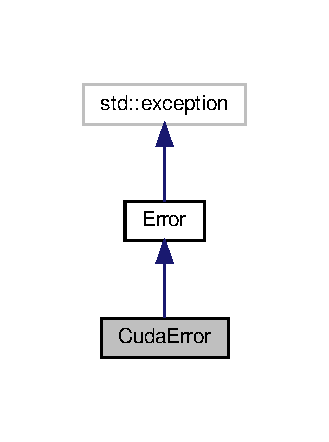
\includegraphics[width=158pt]{classCudaError__coll__graph}
\end{center}
\end{figure}
\subsection*{Public Member Functions}
\begin{DoxyCompactItemize}
\item 
\hyperlink{classCudaError_a90e176d63d838031cb364cdb54532aaf}{Cuda\+Error} (const std\+::string \&file, int line, const std\+::string \&func, int error\+\_\+code)
\begin{DoxyCompactList}\small\item\em Initializes a C\+U\+DA error. \end{DoxyCompactList}\end{DoxyCompactItemize}


\subsection{Detailed Description}
\hyperlink{classCudaError}{Cuda\+Error} is thrown when a C\+U\+DA routine throws a non-\/zero error code. 

\subsection{Constructor \& Destructor Documentation}
\mbox{\Hypertarget{classCudaError_a90e176d63d838031cb364cdb54532aaf}\label{classCudaError_a90e176d63d838031cb364cdb54532aaf}} 
\index{Cuda\+Error@{Cuda\+Error}!Cuda\+Error@{Cuda\+Error}}
\index{Cuda\+Error@{Cuda\+Error}!Cuda\+Error@{Cuda\+Error}}
\subsubsection{\texorpdfstring{Cuda\+Error()}{CudaError()}}
{\footnotesize\ttfamily Cuda\+Error\+::\+Cuda\+Error (\begin{DoxyParamCaption}\item[{const std\+::string \&}]{file,  }\item[{int}]{line,  }\item[{const std\+::string \&}]{func,  }\item[{int}]{error\+\_\+code }\end{DoxyParamCaption})\hspace{0.3cm}{\ttfamily [inline]}}



Initializes a C\+U\+DA error. 


\begin{DoxyParams}{Parameters}
{\em file} & The name of the offending source file \\
\hline
{\em line} & The source code line number where the error occurred \\
\hline
{\em func} & The name of the C\+U\+DA routine that failed \\
\hline
{\em error\+\_\+code} & The resulting C\+U\+DA error code \\
\hline
\end{DoxyParams}


The documentation for this class was generated from the following files\+:\begin{DoxyCompactItemize}
\item 
exception.\+hpp (912c1bd)\item 
/home/runner/work/schwarz-\/lib/schwarz-\/lib/source/exception.\+cpp (912c1bd)\end{DoxyCompactItemize}

\hypertarget{classCusparseError}{}\section{Cusparse\+Error Class Reference}
\label{classCusparseError}\index{Cusparse\+Error@{Cusparse\+Error}}


\hyperlink{classCusparseError}{Cusparse\+Error} is thrown when a cu\+S\+P\+A\+R\+SE routine throws a non-\/zero error code.  




{\ttfamily \#include $<$exception.\+hpp$>$}



Collaboration diagram for Cusparse\+Error\+:
\nopagebreak
\begin{figure}[H]
\begin{center}
\leavevmode
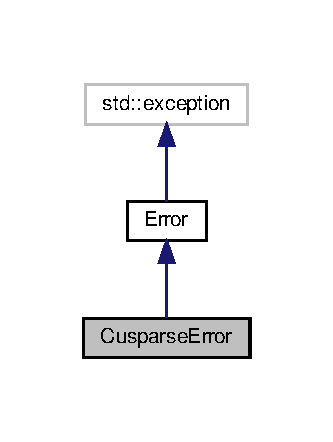
\includegraphics[width=160pt]{classCusparseError__coll__graph}
\end{center}
\end{figure}
\subsection*{Public Member Functions}
\begin{DoxyCompactItemize}
\item 
\hyperlink{classCusparseError_a56df91abf5b97f10bdc6540e06d21617}{Cusparse\+Error} (const std\+::string \&file, int line, const std\+::string \&func, int error\+\_\+code)
\begin{DoxyCompactList}\small\item\em Initializes a cu\+S\+P\+A\+R\+SE error. \end{DoxyCompactList}\end{DoxyCompactItemize}


\subsection{Detailed Description}
\hyperlink{classCusparseError}{Cusparse\+Error} is thrown when a cu\+S\+P\+A\+R\+SE routine throws a non-\/zero error code. 

\subsection{Constructor \& Destructor Documentation}
\mbox{\Hypertarget{classCusparseError_a56df91abf5b97f10bdc6540e06d21617}\label{classCusparseError_a56df91abf5b97f10bdc6540e06d21617}} 
\index{Cusparse\+Error@{Cusparse\+Error}!Cusparse\+Error@{Cusparse\+Error}}
\index{Cusparse\+Error@{Cusparse\+Error}!Cusparse\+Error@{Cusparse\+Error}}
\subsubsection{\texorpdfstring{Cusparse\+Error()}{CusparseError()}}
{\footnotesize\ttfamily Cusparse\+Error\+::\+Cusparse\+Error (\begin{DoxyParamCaption}\item[{const std\+::string \&}]{file,  }\item[{int}]{line,  }\item[{const std\+::string \&}]{func,  }\item[{int}]{error\+\_\+code }\end{DoxyParamCaption})\hspace{0.3cm}{\ttfamily [inline]}}



Initializes a cu\+S\+P\+A\+R\+SE error. 


\begin{DoxyParams}{Parameters}
{\em file} & The name of the offending source file \\
\hline
{\em line} & The source code line number where the error occurred \\
\hline
{\em func} & The name of the cu\+S\+P\+A\+R\+SE routine that failed \\
\hline
{\em error\+\_\+code} & The resulting cu\+S\+P\+A\+R\+SE error code \\
\hline
\end{DoxyParams}


The documentation for this class was generated from the following files\+:\begin{DoxyCompactItemize}
\item 
exception.\+hpp (96003b3)\item 
/home/runner/work/schwarz-\/lib/schwarz-\/lib/source/exception.\+cpp (96003b3)\end{DoxyCompactItemize}

\hypertarget{classschwz_1_1device__guard}{}\section{schwz\+:\+:device\+\_\+guard Class Reference}
\label{classschwz_1_1device__guard}\index{schwz\+::device\+\_\+guard@{schwz\+::device\+\_\+guard}}


This class defines a device guard for the cuda functions and the cuda module.  




{\ttfamily \#include $<$device\+\_\+guard.\+hpp$>$}

\subsection*{Public Member Functions}
\begin{DoxyCompactItemize}
\item 
\mbox{\Hypertarget{classschwz_1_1device__guard_a92b10bc6d8ddd6649dda3766e3daf711}\label{classschwz_1_1device__guard_a92b10bc6d8ddd6649dda3766e3daf711}} 
{\bfseries device\+\_\+guard} (int device\+\_\+id)
\item 
\mbox{\Hypertarget{classschwz_1_1device__guard_a2de09b479828241b2c4a3411c958354c}\label{classschwz_1_1device__guard_a2de09b479828241b2c4a3411c958354c}} 
{\bfseries device\+\_\+guard} (\hyperlink{classschwz_1_1device__guard}{device\+\_\+guard} \&other)=delete
\item 
\mbox{\Hypertarget{classschwz_1_1device__guard_abb46749c09498f2904342dd719451c5a}\label{classschwz_1_1device__guard_abb46749c09498f2904342dd719451c5a}} 
\hyperlink{classschwz_1_1device__guard}{device\+\_\+guard} \& {\bfseries operator=} (const \hyperlink{classschwz_1_1device__guard}{device\+\_\+guard} \&other)=delete
\item 
\mbox{\Hypertarget{classschwz_1_1device__guard_a193c151830543321a641a394099d2249}\label{classschwz_1_1device__guard_a193c151830543321a641a394099d2249}} 
{\bfseries device\+\_\+guard} (\hyperlink{classschwz_1_1device__guard}{device\+\_\+guard} \&\&other)=delete
\item 
\mbox{\Hypertarget{classschwz_1_1device__guard_a54b270cdc45097eceedbc022bbbeed1b}\label{classschwz_1_1device__guard_a54b270cdc45097eceedbc022bbbeed1b}} 
\hyperlink{classschwz_1_1device__guard}{device\+\_\+guard} const  \& {\bfseries operator=} (\hyperlink{classschwz_1_1device__guard}{device\+\_\+guard} \&\&other)=delete
\end{DoxyCompactItemize}


\subsection{Detailed Description}
This class defines a device guard for the cuda functions and the cuda module. 

The guard is used to make sure that the device code is run on the correct cuda device, when run with multiple devices. The class records the current device id and uses {\ttfamily cuda\+Set\+Device} to set the device id to the one being passed in. After the scope has been exited, the destructor sets the device\+\_\+id back to the one before entering the scope. 

The documentation for this class was generated from the following file\+:\begin{DoxyCompactItemize}
\item 
device\+\_\+guard.\+hpp (5af933a)\end{DoxyCompactItemize}

\hypertarget{classError}{}\section{Error Class Reference}
\label{classError}\index{Error@{Error}}


Collaboration diagram for Error\+:
\nopagebreak
\begin{figure}[H]
\begin{center}
\leavevmode
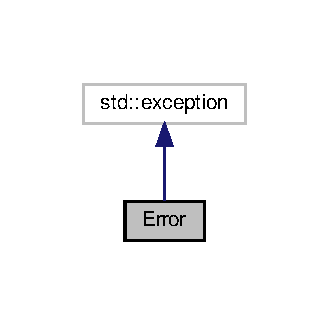
\includegraphics[width=158pt]{classError__coll__graph}
\end{center}
\end{figure}
\subsection*{Public Member Functions}
\begin{DoxyCompactItemize}
\item 
\hyperlink{classError_a146e7d37cbd73162b88a91ffa7fa776a}{Error} (const std\+::string \&file, int line, const std\+::string \&\hyperlink{classError_aeca4bfa7822e73acddcb68276dc1f306}{what})
\begin{DoxyCompactList}\small\item\em Initializes an error. \end{DoxyCompactList}\item 
\mbox{\Hypertarget{classError_aeca4bfa7822e73acddcb68276dc1f306}\label{classError_aeca4bfa7822e73acddcb68276dc1f306}} 
virtual const char $\ast$ \hyperlink{classError_aeca4bfa7822e73acddcb68276dc1f306}{what} () const noexcept override
\begin{DoxyCompactList}\small\item\em Returns a human-\/readable string with a more detailed description of the error. \end{DoxyCompactList}\end{DoxyCompactItemize}


\subsection{Constructor \& Destructor Documentation}
\mbox{\Hypertarget{classError_a146e7d37cbd73162b88a91ffa7fa776a}\label{classError_a146e7d37cbd73162b88a91ffa7fa776a}} 
\index{Error@{Error}!Error@{Error}}
\index{Error@{Error}!Error@{Error}}
\subsubsection{\texorpdfstring{Error()}{Error()}}
{\footnotesize\ttfamily Error\+::\+Error (\begin{DoxyParamCaption}\item[{const std\+::string \&}]{file,  }\item[{int}]{line,  }\item[{const std\+::string \&}]{what }\end{DoxyParamCaption})\hspace{0.3cm}{\ttfamily [inline]}}



Initializes an error. 


\begin{DoxyParams}{Parameters}
{\em file} & The name of the offending source file \\
\hline
{\em line} & The source code line number where the error occurred \\
\hline
{\em what} & The error message \\
\hline
\end{DoxyParams}


The documentation for this class was generated from the following file\+:\begin{DoxyCompactItemize}
\item 
exception.\+hpp (65b21a9)\end{DoxyCompactItemize}

\hypertarget{structschwz_1_1Gather}{}\section{schwz\+:\+:Gather$<$ Value\+Type, Index\+Type $>$ Struct Template Reference}
\label{structschwz_1_1Gather}\index{schwz\+::\+Gather$<$ Value\+Type, Index\+Type $>$@{schwz\+::\+Gather$<$ Value\+Type, Index\+Type $>$}}


Collaboration diagram for schwz\+:\+:Gather$<$ Value\+Type, Index\+Type $>$\+:
\nopagebreak
\begin{figure}[H]
\begin{center}
\leavevmode
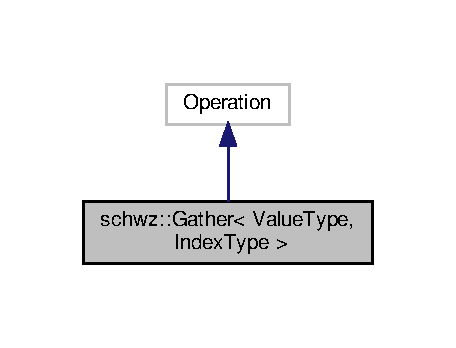
\includegraphics[width=219pt]{structschwz_1_1Gather__coll__graph}
\end{center}
\end{figure}
\subsection*{Public Member Functions}
\begin{DoxyCompactItemize}
\item 
\mbox{\Hypertarget{structschwz_1_1Gather_abd8ae2ad78e73b0e5b47d5bbc02f7306}\label{structschwz_1_1Gather_abd8ae2ad78e73b0e5b47d5bbc02f7306}} 
{\bfseries Gather} (const Index\+Type num\+\_\+elems, const Index\+Type $\ast$indices, const Value\+Type $\ast$from\+\_\+array, Value\+Type $\ast$into\+\_\+array, Operation\+Type optype)
\item 
\mbox{\Hypertarget{structschwz_1_1Gather_a78567471344a9c03fabc5868431a5338}\label{structschwz_1_1Gather_a78567471344a9c03fabc5868431a5338}} 
void {\bfseries run} (std\+::shared\+\_\+ptr$<$ const gko\+::\+Omp\+Executor $>$) const override
\item 
\mbox{\Hypertarget{structschwz_1_1Gather_a2ba1eb7e12a81bbee46bf0df67ad6640}\label{structschwz_1_1Gather_a2ba1eb7e12a81bbee46bf0df67ad6640}} 
void {\bfseries run} (std\+::shared\+\_\+ptr$<$ const gko\+::\+Cuda\+Executor $>$) const override
\end{DoxyCompactItemize}
\subsection*{Public Attributes}
\begin{DoxyCompactItemize}
\item 
\mbox{\Hypertarget{structschwz_1_1Gather_a9c16149747d5a4c77c061d750a27faf2}\label{structschwz_1_1Gather_a9c16149747d5a4c77c061d750a27faf2}} 
const Index\+Type {\bfseries num\+\_\+elems}
\item 
\mbox{\Hypertarget{structschwz_1_1Gather_a8adc05f74bac862e80eae9e5bcd6918d}\label{structschwz_1_1Gather_a8adc05f74bac862e80eae9e5bcd6918d}} 
const Index\+Type $\ast$ {\bfseries indices}
\item 
\mbox{\Hypertarget{structschwz_1_1Gather_ae45f6ecca9f53252e804c6de1b96f4dd}\label{structschwz_1_1Gather_ae45f6ecca9f53252e804c6de1b96f4dd}} 
const Value\+Type $\ast$ {\bfseries from\+\_\+array}
\item 
\mbox{\Hypertarget{structschwz_1_1Gather_a2edcfcb6bb277db9273a3865a4c2f017}\label{structschwz_1_1Gather_a2edcfcb6bb277db9273a3865a4c2f017}} 
Value\+Type $\ast$ {\bfseries into\+\_\+array}
\item 
\mbox{\Hypertarget{structschwz_1_1Gather_a8830fdf0a3d07abb1d985fa4cb42bb08}\label{structschwz_1_1Gather_a8830fdf0a3d07abb1d985fa4cb42bb08}} 
Operation\+Type {\bfseries optype}
\end{DoxyCompactItemize}


The documentation for this struct was generated from the following file\+:\begin{DoxyCompactItemize}
\item 
gather.\+hpp (9d4939f)\end{DoxyCompactItemize}

\hypertarget{classschwz_1_1Initialize}{}\section{schwz\+:\+:Initialize$<$ Value\+Type, Index\+Type $>$ Class Template Reference}
\label{classschwz_1_1Initialize}\index{schwz\+::\+Initialize$<$ Value\+Type, Index\+Type $>$@{schwz\+::\+Initialize$<$ Value\+Type, Index\+Type $>$}}


The initialization class that provides methods for initialization of the solver.  




{\ttfamily \#include $<$initialization.\+hpp$>$}



Collaboration diagram for schwz\+:\+:Initialize$<$ Value\+Type, Index\+Type $>$\+:
\nopagebreak
\begin{figure}[H]
\begin{center}
\leavevmode
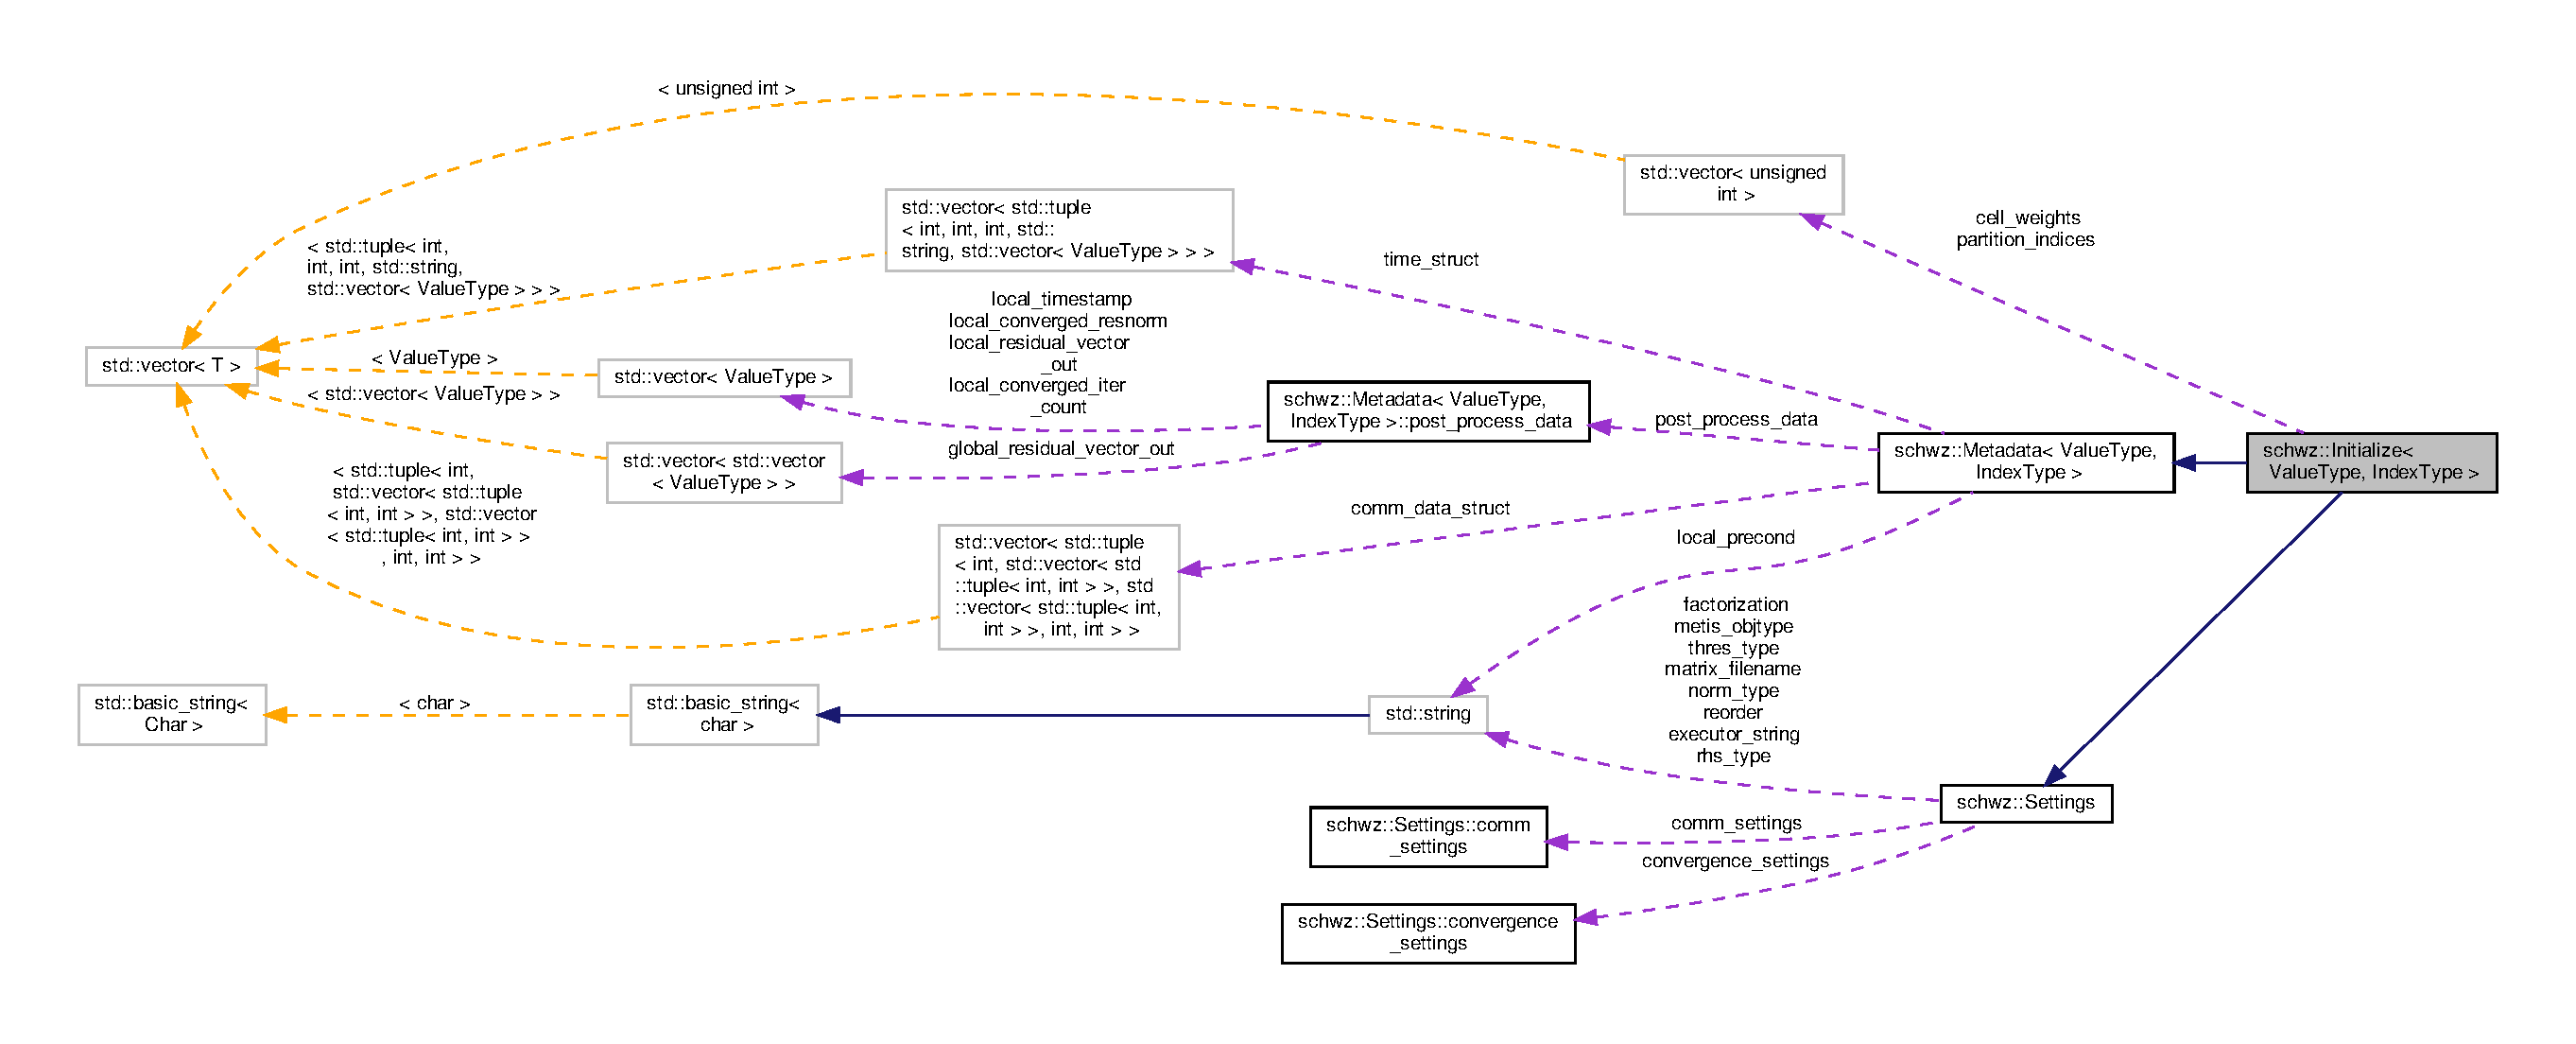
\includegraphics[width=350pt]{classschwz_1_1Initialize__coll__graph}
\end{center}
\end{figure}
\subsection*{Public Member Functions}
\begin{DoxyCompactItemize}
\item 
\mbox{\Hypertarget{classschwz_1_1Initialize_a8ebf7bcf4c67d4ca6af0b5afba5a9a90}\label{classschwz_1_1Initialize_a8ebf7bcf4c67d4ca6af0b5afba5a9a90}} 
{\bfseries Initialize} (\hyperlink{structschwz_1_1Settings}{Settings} \&settings, \hyperlink{structschwz_1_1Metadata}{Metadata}$<$ Value\+Type, Index\+Type $>$ \&metadata)
\item 
void \hyperlink{classschwz_1_1Initialize_a9dee6b55c599df30410cdf45819b3e28}{generate\+\_\+rhs} (std\+::vector$<$ Value\+Type $>$ \&rhs)
\begin{DoxyCompactList}\small\item\em Generates the right hand side vector. \end{DoxyCompactList}\item 
void \hyperlink{classschwz_1_1Initialize_af655816bbed181e0a243efa7e35e942f}{setup\+\_\+global\+\_\+matrix} (const std\+::string \&filename, const gko\+::size\+\_\+type \&\hyperlink{structschwz_1_1Metadata_a1333605c0573688ce4d71173f52ef2b4}{oned\+\_\+laplacian\+\_\+size}, std\+::shared\+\_\+ptr$<$ gko\+::matrix\+::\+Csr$<$ Value\+Type, Index\+Type $>$$>$ \&global\+\_\+matrix)
\begin{DoxyCompactList}\small\item\em Generates the 2D global laplacian matrix. \end{DoxyCompactList}\item 
void \hyperlink{classschwz_1_1Initialize_a23a10058e35a442c564c0748b66dcb08}{partition} (const \hyperlink{structschwz_1_1Settings}{Settings} \&settings, const \hyperlink{structschwz_1_1Metadata}{Metadata}$<$ Value\+Type, Index\+Type $>$ \&metadata, const std\+::shared\+\_\+ptr$<$ gko\+::matrix\+::\+Csr$<$ Value\+Type, Index\+Type $>$$>$ \&global\+\_\+matrix, std\+::vector$<$ unsigned int $>$ \&\hyperlink{classschwz_1_1Initialize_a007426e21221298b6dca9b7c9fbd1c10}{partition\+\_\+indices})
\begin{DoxyCompactList}\small\item\em The partitioning function. \end{DoxyCompactList}\item 
void \hyperlink{classschwz_1_1Initialize_af8e2c507404900e2507f6b44b16ca4b7}{setup\+\_\+vectors} (const \hyperlink{structschwz_1_1Settings}{Settings} \&settings, const \hyperlink{structschwz_1_1Metadata}{Metadata}$<$ Value\+Type, Index\+Type $>$ \&metadata, std\+::vector$<$ Value\+Type $>$ \&rhs, std\+::shared\+\_\+ptr$<$ gko\+::matrix\+::\+Dense$<$ Value\+Type $>$$>$ \&local\+\_\+rhs, std\+::shared\+\_\+ptr$<$ gko\+::matrix\+::\+Dense$<$ Value\+Type $>$$>$ \&global\+\_\+rhs, std\+::shared\+\_\+ptr$<$ gko\+::matrix\+::\+Dense$<$ Value\+Type $>$$>$ \&local\+\_\+solution)
\begin{DoxyCompactList}\small\item\em Setup the vectors with default values and allocate mameory if not allocated. \end{DoxyCompactList}\item 
virtual void \hyperlink{classschwz_1_1Initialize_ad24764a4ded54c2af6a5111ba8c8228f}{setup\+\_\+local\+\_\+matrices} (\hyperlink{structschwz_1_1Settings}{Settings} \&settings, \hyperlink{structschwz_1_1Metadata}{Metadata}$<$ Value\+Type, Index\+Type $>$ \&metadata, std\+::vector$<$ unsigned int $>$ \&\hyperlink{classschwz_1_1Initialize_a007426e21221298b6dca9b7c9fbd1c10}{partition\+\_\+indices}, std\+::shared\+\_\+ptr$<$ gko\+::matrix\+::\+Csr$<$ Value\+Type, Index\+Type $>$$>$ \&global\+\_\+matrix, std\+::shared\+\_\+ptr$<$ gko\+::matrix\+::\+Csr$<$ Value\+Type, Index\+Type $>$$>$ \&local\+\_\+matrix, std\+::shared\+\_\+ptr$<$ gko\+::matrix\+::\+Csr$<$ Value\+Type, Index\+Type $>$$>$ \&interface\+\_\+matrix)=0
\begin{DoxyCompactList}\small\item\em Sets up the local and the interface matrices from the global matrix and the partition indices. \end{DoxyCompactList}\end{DoxyCompactItemize}
\subsection*{Public Attributes}
\begin{DoxyCompactItemize}
\item 
\mbox{\Hypertarget{classschwz_1_1Initialize_a007426e21221298b6dca9b7c9fbd1c10}\label{classschwz_1_1Initialize_a007426e21221298b6dca9b7c9fbd1c10}} 
std\+::vector$<$ unsigned int $>$ \hyperlink{classschwz_1_1Initialize_a007426e21221298b6dca9b7c9fbd1c10}{partition\+\_\+indices}
\begin{DoxyCompactList}\small\item\em The partition indices containing the subdomains to which each row(vertex) of the matrix(graph) belongs to. \end{DoxyCompactList}\item 
\mbox{\Hypertarget{classschwz_1_1Initialize_a715b9e3a552f77277492d1c86c600681}\label{classschwz_1_1Initialize_a715b9e3a552f77277492d1c86c600681}} 
std\+::vector$<$ unsigned int $>$ \hyperlink{classschwz_1_1Initialize_a715b9e3a552f77277492d1c86c600681}{cell\+\_\+weights}
\begin{DoxyCompactList}\small\item\em The cell weights for the partition algorithm. \end{DoxyCompactList}\end{DoxyCompactItemize}
\subsection*{Additional Inherited Members}


\subsection{Detailed Description}
\subsubsection*{template$<$typename Value\+Type = gko\+::default\+\_\+precision, typename Index\+Type = gko\+::int32$>$\newline
class schwz\+::\+Initialize$<$ Value\+Type, Index\+Type $>$}

The initialization class that provides methods for initialization of the solver. 


\begin{DoxyTemplParams}{Template Parameters}
{\em Value\+Type} & The type of the floating point values. \\
\hline
{\em Index\+Type} & The type of the index type values.\\
\hline
\end{DoxyTemplParams}
\hyperlink{group__init}{Initialization} 

\subsection{Member Function Documentation}
\mbox{\Hypertarget{classschwz_1_1Initialize_a9dee6b55c599df30410cdf45819b3e28}\label{classschwz_1_1Initialize_a9dee6b55c599df30410cdf45819b3e28}} 
\index{schwz\+::\+Initialize@{schwz\+::\+Initialize}!generate\+\_\+rhs@{generate\+\_\+rhs}}
\index{generate\+\_\+rhs@{generate\+\_\+rhs}!schwz\+::\+Initialize@{schwz\+::\+Initialize}}
\subsubsection{\texorpdfstring{generate\+\_\+rhs()}{generate\_rhs()}}
{\footnotesize\ttfamily template$<$typename Value\+Type , typename Index\+Type $>$ \\
void \hyperlink{classschwz_1_1Initialize}{schwz\+::\+Initialize}$<$ Value\+Type, Index\+Type $>$\+::generate\+\_\+rhs (\begin{DoxyParamCaption}\item[{std\+::vector$<$ Value\+Type $>$ \&}]{rhs }\end{DoxyParamCaption})}



Generates the right hand side vector. 


\begin{DoxyParams}{Parameters}
{\em rhs} & The rhs vector. \\
\hline
\end{DoxyParams}


References schwz\+::\+Initialize$<$ Value\+Type, Index\+Type $>$\+::setup\+\_\+global\+\_\+matrix().



Referenced by schwz\+::\+Schwarz\+Base$<$ Value\+Type, Index\+Type, Mixed\+Value\+Type $>$\+::initialize().

\mbox{\Hypertarget{classschwz_1_1Initialize_a23a10058e35a442c564c0748b66dcb08}\label{classschwz_1_1Initialize_a23a10058e35a442c564c0748b66dcb08}} 
\index{schwz\+::\+Initialize@{schwz\+::\+Initialize}!partition@{partition}}
\index{partition@{partition}!schwz\+::\+Initialize@{schwz\+::\+Initialize}}
\subsubsection{\texorpdfstring{partition()}{partition()}}
{\footnotesize\ttfamily template$<$typename Value\+Type , typename Index\+Type $>$ \\
void \hyperlink{classschwz_1_1Initialize}{schwz\+::\+Initialize}$<$ Value\+Type, Index\+Type $>$\+::partition (\begin{DoxyParamCaption}\item[{const \hyperlink{structschwz_1_1Settings}{Settings} \&}]{settings,  }\item[{const \hyperlink{structschwz_1_1Metadata}{Metadata}$<$ Value\+Type, Index\+Type $>$ \&}]{metadata,  }\item[{const std\+::shared\+\_\+ptr$<$ gko\+::matrix\+::\+Csr$<$ Value\+Type, Index\+Type $>$$>$ \&}]{global\+\_\+matrix,  }\item[{std\+::vector$<$ unsigned int $>$ \&}]{partition\+\_\+indices }\end{DoxyParamCaption})}



The partitioning function. 

Allows the partition of the global matrix depending with M\+E\+T\+IS and a regular 1D decomposition.


\begin{DoxyParams}{Parameters}
{\em settings} & The settings struct. \\
\hline
{\em metadata} & The metadata struct. \\
\hline
{\em global\+\_\+matrix} & The global matrix. \\
\hline
{\em partition\+\_\+indices} & The partition indices \mbox{[}O\+U\+T\+P\+UT\mbox{]}. \\
\hline
\end{DoxyParams}


References schwz\+::\+Metadata$<$ Value\+Type, Index\+Type $>$\+::global\+\_\+size, schwz\+::\+Metadata$<$ Value\+Type, Index\+Type $>$\+::my\+\_\+rank, schwz\+::\+Metadata$<$ Value\+Type, Index\+Type $>$\+::num\+\_\+subdomains, and schwz\+::\+Settings\+::write\+\_\+debug\+\_\+out.



Referenced by schwz\+::\+Schwarz\+Base$<$ Value\+Type, Index\+Type, Mixed\+Value\+Type $>$\+::initialize().

\mbox{\Hypertarget{classschwz_1_1Initialize_af655816bbed181e0a243efa7e35e942f}\label{classschwz_1_1Initialize_af655816bbed181e0a243efa7e35e942f}} 
\index{schwz\+::\+Initialize@{schwz\+::\+Initialize}!setup\+\_\+global\+\_\+matrix@{setup\+\_\+global\+\_\+matrix}}
\index{setup\+\_\+global\+\_\+matrix@{setup\+\_\+global\+\_\+matrix}!schwz\+::\+Initialize@{schwz\+::\+Initialize}}
\subsubsection{\texorpdfstring{setup\+\_\+global\+\_\+matrix()}{setup\_global\_matrix()}}
{\footnotesize\ttfamily template$<$typename Value\+Type , typename Index\+Type $>$ \\
void \hyperlink{classschwz_1_1Initialize}{schwz\+::\+Initialize}$<$ Value\+Type, Index\+Type $>$\+::setup\+\_\+global\+\_\+matrix (\begin{DoxyParamCaption}\item[{const std\+::string \&}]{filename,  }\item[{const gko\+::size\+\_\+type \&}]{oned\+\_\+laplacian\+\_\+size,  }\item[{std\+::shared\+\_\+ptr$<$ gko\+::matrix\+::\+Csr$<$ Value\+Type, Index\+Type $>$$>$ \&}]{global\+\_\+matrix }\end{DoxyParamCaption})}



Generates the 2D global laplacian matrix. 


\begin{DoxyParams}{Parameters}
{\em oned\+\_\+laplacian\+\_\+size} & The size of the one d laplacian grid. \\
\hline
{\em global\+\_\+matrix} & The global matrix. \\
\hline
\end{DoxyParams}


Referenced by schwz\+::\+Initialize$<$ Value\+Type, Index\+Type $>$\+::generate\+\_\+rhs(), and schwz\+::\+Schwarz\+Base$<$ Value\+Type, Index\+Type, Mixed\+Value\+Type $>$\+::initialize().

\mbox{\Hypertarget{classschwz_1_1Initialize_ad24764a4ded54c2af6a5111ba8c8228f}\label{classschwz_1_1Initialize_ad24764a4ded54c2af6a5111ba8c8228f}} 
\index{schwz\+::\+Initialize@{schwz\+::\+Initialize}!setup\+\_\+local\+\_\+matrices@{setup\+\_\+local\+\_\+matrices}}
\index{setup\+\_\+local\+\_\+matrices@{setup\+\_\+local\+\_\+matrices}!schwz\+::\+Initialize@{schwz\+::\+Initialize}}
\subsubsection{\texorpdfstring{setup\+\_\+local\+\_\+matrices()}{setup\_local\_matrices()}}
{\footnotesize\ttfamily template$<$typename Value\+Type , typename Index\+Type $>$ \\
void \hyperlink{classschwz_1_1Initialize}{schwz\+::\+Initialize}$<$ Value\+Type, Index\+Type $>$\+::setup\+\_\+local\+\_\+matrices (\begin{DoxyParamCaption}\item[{\hyperlink{structschwz_1_1Settings}{Settings} \&}]{settings,  }\item[{\hyperlink{structschwz_1_1Metadata}{Metadata}$<$ Value\+Type, Index\+Type $>$ \&}]{metadata,  }\item[{std\+::vector$<$ unsigned int $>$ \&}]{partition\+\_\+indices,  }\item[{std\+::shared\+\_\+ptr$<$ gko\+::matrix\+::\+Csr$<$ Value\+Type, Index\+Type $>$$>$ \&}]{global\+\_\+matrix,  }\item[{std\+::shared\+\_\+ptr$<$ gko\+::matrix\+::\+Csr$<$ Value\+Type, Index\+Type $>$$>$ \&}]{local\+\_\+matrix,  }\item[{std\+::shared\+\_\+ptr$<$ gko\+::matrix\+::\+Csr$<$ Value\+Type, Index\+Type $>$$>$ \&}]{interface\+\_\+matrix }\end{DoxyParamCaption})\hspace{0.3cm}{\ttfamily [pure virtual]}}



Sets up the local and the interface matrices from the global matrix and the partition indices. 


\begin{DoxyParams}{Parameters}
{\em settings} & The settings struct. \\
\hline
{\em metadata} & The metadata struct. \\
\hline
{\em partition\+\_\+indices} & The array containing the partition indices. \\
\hline
{\em global\+\_\+matrix} & The global system matrix. \\
\hline
{\em local\+\_\+matrix} & The local system matrix. \\
\hline
{\em interface\+\_\+matrix} & The interface matrix containing the interface and the overlap data mainly used for exchanging values between different sub-\/domains. \\
\hline
{\em local\+\_\+perm} & The local permutation, obtained through R\+CM or M\+E\+T\+IS. \\
\hline
\end{DoxyParams}


Implemented in \hyperlink{classschwz_1_1SolverRAS_ab31f86ccc8300a0212eca77c91de132a}{schwz\+::\+Solver\+R\+A\+S$<$ Value\+Type, Index\+Type, Mixed\+Value\+Type $>$}.



Referenced by schwz\+::\+Schwarz\+Base$<$ Value\+Type, Index\+Type, Mixed\+Value\+Type $>$\+::initialize().

\mbox{\Hypertarget{classschwz_1_1Initialize_af8e2c507404900e2507f6b44b16ca4b7}\label{classschwz_1_1Initialize_af8e2c507404900e2507f6b44b16ca4b7}} 
\index{schwz\+::\+Initialize@{schwz\+::\+Initialize}!setup\+\_\+vectors@{setup\+\_\+vectors}}
\index{setup\+\_\+vectors@{setup\+\_\+vectors}!schwz\+::\+Initialize@{schwz\+::\+Initialize}}
\subsubsection{\texorpdfstring{setup\+\_\+vectors()}{setup\_vectors()}}
{\footnotesize\ttfamily template$<$typename Value\+Type , typename Index\+Type $>$ \\
void \hyperlink{classschwz_1_1Initialize}{schwz\+::\+Initialize}$<$ Value\+Type, Index\+Type $>$\+::setup\+\_\+vectors (\begin{DoxyParamCaption}\item[{const \hyperlink{structschwz_1_1Settings}{Settings} \&}]{settings,  }\item[{const \hyperlink{structschwz_1_1Metadata}{Metadata}$<$ Value\+Type, Index\+Type $>$ \&}]{metadata,  }\item[{std\+::vector$<$ Value\+Type $>$ \&}]{rhs,  }\item[{std\+::shared\+\_\+ptr$<$ gko\+::matrix\+::\+Dense$<$ Value\+Type $>$$>$ \&}]{local\+\_\+rhs,  }\item[{std\+::shared\+\_\+ptr$<$ gko\+::matrix\+::\+Dense$<$ Value\+Type $>$$>$ \&}]{global\+\_\+rhs,  }\item[{std\+::shared\+\_\+ptr$<$ gko\+::matrix\+::\+Dense$<$ Value\+Type $>$$>$ \&}]{local\+\_\+solution }\end{DoxyParamCaption})}



Setup the vectors with default values and allocate mameory if not allocated. 


\begin{DoxyParams}{Parameters}
{\em settings} & The settings struct. \\
\hline
{\em metadata} & The metadata struct. \\
\hline
{\em local\+\_\+rhs} & The local right hand side vector in the subdomain. \\
\hline
{\em global\+\_\+rhs} & The global right hand side vector. \\
\hline
{\em local\+\_\+solution} & The local solution vector in the subdomain. \\
\hline
\end{DoxyParams}


References schwz\+::\+Settings\+::executor, schwz\+::\+Metadata$<$ Value\+Type, Index\+Type $>$\+::first\+\_\+row, schwz\+::\+Metadata$<$ Value\+Type, Index\+Type $>$\+::local\+\_\+size\+\_\+x, and schwz\+::\+Metadata$<$ Value\+Type, Index\+Type $>$\+::my\+\_\+rank.



Referenced by schwz\+::\+Schwarz\+Base$<$ Value\+Type, Index\+Type, Mixed\+Value\+Type $>$\+::initialize().



The documentation for this class was generated from the following files\+:\begin{DoxyCompactItemize}
\item 
initialization.\+hpp (7c9a9f7)\item 
/home/runner/work/schwarz-\/lib/schwarz-\/lib/source/initialization.\+cpp (7c9a9f7)\end{DoxyCompactItemize}

\hypertarget{structschwz_1_1Metadata}{}\section{schwz\+:\+:Metadata$<$ Value\+Type, Index\+Type $>$ Struct Template Reference}
\label{structschwz_1_1Metadata}\index{schwz\+::\+Metadata$<$ Value\+Type, Index\+Type $>$@{schwz\+::\+Metadata$<$ Value\+Type, Index\+Type $>$}}


The solver metadata struct.  




{\ttfamily \#include $<$settings.\+hpp$>$}



Collaboration diagram for schwz\+:\+:Metadata$<$ Value\+Type, Index\+Type $>$\+:
\nopagebreak
\begin{figure}[H]
\begin{center}
\leavevmode
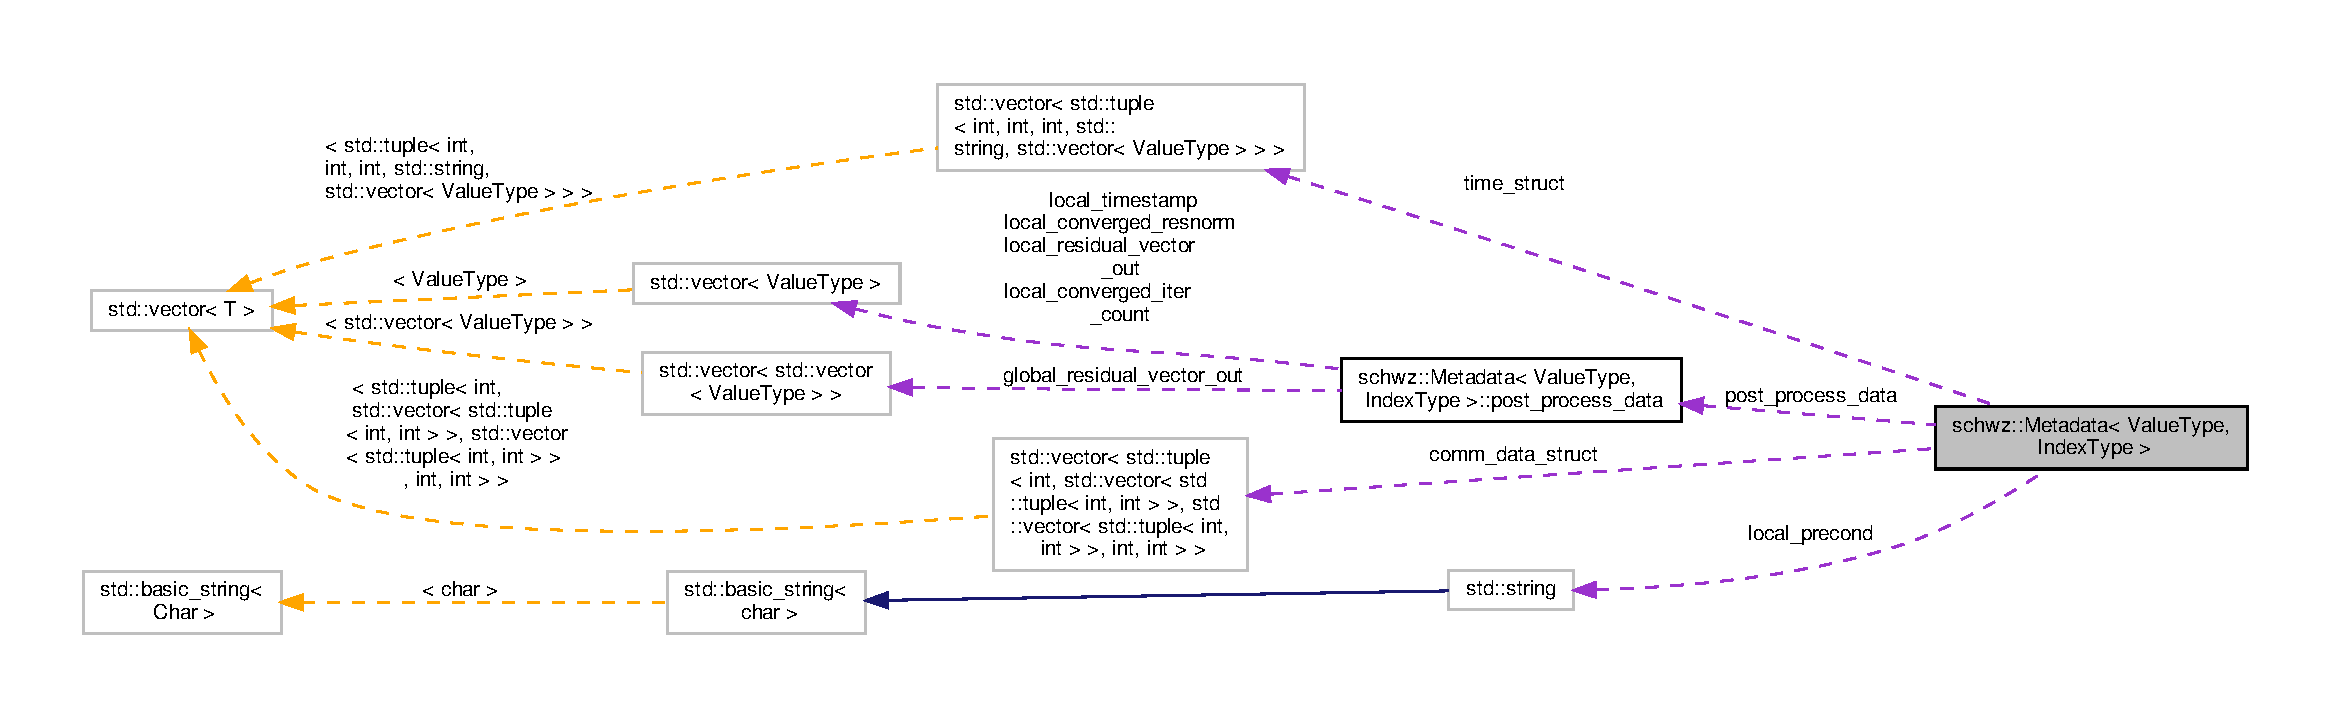
\includegraphics[width=350pt]{structschwz_1_1Metadata__coll__graph}
\end{center}
\end{figure}
\subsection*{Classes}
\begin{DoxyCompactItemize}
\item 
struct \hyperlink{structschwz_1_1Metadata_1_1post__process__data}{post\+\_\+process\+\_\+data}
\begin{DoxyCompactList}\small\item\em The struct used for storing data for post-\/processing. \end{DoxyCompactList}\end{DoxyCompactItemize}
\subsection*{Public Attributes}
\begin{DoxyCompactItemize}
\item 
\mbox{\Hypertarget{structschwz_1_1Metadata_a84a525a7a5f5282dcc1ef165e93bad35}\label{structschwz_1_1Metadata_a84a525a7a5f5282dcc1ef165e93bad35}} 
M\+P\+I\+\_\+\+Comm \hyperlink{structschwz_1_1Metadata_a84a525a7a5f5282dcc1ef165e93bad35}{mpi\+\_\+communicator}
\begin{DoxyCompactList}\small\item\em The M\+PI communicator. \end{DoxyCompactList}\item 
\mbox{\Hypertarget{structschwz_1_1Metadata_a9c8057649291f015a29e246dc9b0dca4}\label{structschwz_1_1Metadata_a9c8057649291f015a29e246dc9b0dca4}} 
gko\+::size\+\_\+type \hyperlink{structschwz_1_1Metadata_a9c8057649291f015a29e246dc9b0dca4}{global\+\_\+size} = 0
\begin{DoxyCompactList}\small\item\em The size of the global matrix. \end{DoxyCompactList}\item 
\mbox{\Hypertarget{structschwz_1_1Metadata_a1333605c0573688ce4d71173f52ef2b4}\label{structschwz_1_1Metadata_a1333605c0573688ce4d71173f52ef2b4}} 
gko\+::size\+\_\+type \hyperlink{structschwz_1_1Metadata_a1333605c0573688ce4d71173f52ef2b4}{oned\+\_\+laplacian\+\_\+size} = 0
\begin{DoxyCompactList}\small\item\em The size of the 1 dimensional laplacian grid. \end{DoxyCompactList}\item 
\mbox{\Hypertarget{structschwz_1_1Metadata_a1e24cc843abc923c309fb74243323d8c}\label{structschwz_1_1Metadata_a1e24cc843abc923c309fb74243323d8c}} 
gko\+::size\+\_\+type \hyperlink{structschwz_1_1Metadata_a1e24cc843abc923c309fb74243323d8c}{local\+\_\+size} = 0
\begin{DoxyCompactList}\small\item\em The size of the local subdomain matrix. \end{DoxyCompactList}\item 
\mbox{\Hypertarget{structschwz_1_1Metadata_a64639c8f3ff4c240e50a3862e95303dc}\label{structschwz_1_1Metadata_a64639c8f3ff4c240e50a3862e95303dc}} 
gko\+::size\+\_\+type \hyperlink{structschwz_1_1Metadata_a64639c8f3ff4c240e50a3862e95303dc}{local\+\_\+size\+\_\+x} = 0
\begin{DoxyCompactList}\small\item\em The size of the local subdomain matrix + the overlap. \end{DoxyCompactList}\item 
\mbox{\Hypertarget{structschwz_1_1Metadata_ad5cf4b6c627cb4f5be927f2c968c7e0d}\label{structschwz_1_1Metadata_ad5cf4b6c627cb4f5be927f2c968c7e0d}} 
gko\+::size\+\_\+type \hyperlink{structschwz_1_1Metadata_ad5cf4b6c627cb4f5be927f2c968c7e0d}{local\+\_\+size\+\_\+o} = 0
\begin{DoxyCompactList}\small\item\em The size of the local subdomain matrix + the overlap. \end{DoxyCompactList}\item 
\mbox{\Hypertarget{structschwz_1_1Metadata_ad1d2e8aadc49157a91b0deabda53621e}\label{structschwz_1_1Metadata_ad1d2e8aadc49157a91b0deabda53621e}} 
gko\+::size\+\_\+type \hyperlink{structschwz_1_1Metadata_ad1d2e8aadc49157a91b0deabda53621e}{overlap\+\_\+size} = 0
\begin{DoxyCompactList}\small\item\em The size of the overlap between the subdomains. \end{DoxyCompactList}\item 
\mbox{\Hypertarget{structschwz_1_1Metadata_aaba09003a5ffa4e8770d5f9f76d69d6b}\label{structschwz_1_1Metadata_aaba09003a5ffa4e8770d5f9f76d69d6b}} 
gko\+::size\+\_\+type \hyperlink{structschwz_1_1Metadata_aaba09003a5ffa4e8770d5f9f76d69d6b}{num\+\_\+subdomains} = 1
\begin{DoxyCompactList}\small\item\em The number of subdomains used within the solver. \end{DoxyCompactList}\item 
\mbox{\Hypertarget{structschwz_1_1Metadata_ac8ebd3ef6215f782ad5179b46994533f}\label{structschwz_1_1Metadata_ac8ebd3ef6215f782ad5179b46994533f}} 
int \hyperlink{structschwz_1_1Metadata_ac8ebd3ef6215f782ad5179b46994533f}{my\+\_\+rank}
\begin{DoxyCompactList}\small\item\em The rank of the subdomain. \end{DoxyCompactList}\item 
\mbox{\Hypertarget{structschwz_1_1Metadata_a8e48fee48d4865f2a23782e2bf3e9f5c}\label{structschwz_1_1Metadata_a8e48fee48d4865f2a23782e2bf3e9f5c}} 
int \hyperlink{structschwz_1_1Metadata_a8e48fee48d4865f2a23782e2bf3e9f5c}{my\+\_\+local\+\_\+rank}
\begin{DoxyCompactList}\small\item\em The local rank of the subdomain. \end{DoxyCompactList}\item 
\mbox{\Hypertarget{structschwz_1_1Metadata_a1023b28f7655d4053423d75d0e98eee8}\label{structschwz_1_1Metadata_a1023b28f7655d4053423d75d0e98eee8}} 
int \hyperlink{structschwz_1_1Metadata_a1023b28f7655d4053423d75d0e98eee8}{local\+\_\+num\+\_\+procs}
\begin{DoxyCompactList}\small\item\em The local number of procs in the subdomain. \end{DoxyCompactList}\item 
\mbox{\Hypertarget{structschwz_1_1Metadata_aae2c0f118e53c26239ada9c3f71b0eae}\label{structschwz_1_1Metadata_aae2c0f118e53c26239ada9c3f71b0eae}} 
int \hyperlink{structschwz_1_1Metadata_aae2c0f118e53c26239ada9c3f71b0eae}{comm\+\_\+size}
\begin{DoxyCompactList}\small\item\em The number of subdomains used within the solver, size of the communicator. \end{DoxyCompactList}\item 
\mbox{\Hypertarget{structschwz_1_1Metadata_ac6a6052778d497a1d1aa9804c0bd28bc}\label{structschwz_1_1Metadata_ac6a6052778d497a1d1aa9804c0bd28bc}} 
int \hyperlink{structschwz_1_1Metadata_ac6a6052778d497a1d1aa9804c0bd28bc}{num\+\_\+threads}
\begin{DoxyCompactList}\small\item\em The number of threads used within the solver for each subdomain. \end{DoxyCompactList}\item 
\mbox{\Hypertarget{structschwz_1_1Metadata_acd8efc17b3d0a1804dc0a5bf40af586c}\label{structschwz_1_1Metadata_acd8efc17b3d0a1804dc0a5bf40af586c}} 
Index\+Type \hyperlink{structschwz_1_1Metadata_acd8efc17b3d0a1804dc0a5bf40af586c}{iter\+\_\+count}
\begin{DoxyCompactList}\small\item\em The iteration count of the solver. \end{DoxyCompactList}\item 
Value\+Type \hyperlink{structschwz_1_1Metadata_a366db94e2a75dbdd82616e0d0b33bb86}{tolerance}
\begin{DoxyCompactList}\small\item\em The tolerance of the complete solver. \end{DoxyCompactList}\item 
Value\+Type \hyperlink{structschwz_1_1Metadata_a0fec5924fa99f07cabf560cc461887b5}{local\+\_\+solver\+\_\+tolerance}
\begin{DoxyCompactList}\small\item\em The tolerance of the local solver in case of an iterative solve. \end{DoxyCompactList}\item 
\mbox{\Hypertarget{structschwz_1_1Metadata_aa3fbf70891e008cf810b6480be6607da}\label{structschwz_1_1Metadata_aa3fbf70891e008cf810b6480be6607da}} 
Index\+Type \hyperlink{structschwz_1_1Metadata_aa3fbf70891e008cf810b6480be6607da}{max\+\_\+iters}
\begin{DoxyCompactList}\small\item\em The maximum iteration count of the Schwarz solver. \end{DoxyCompactList}\item 
\mbox{\Hypertarget{structschwz_1_1Metadata_a54d674e16789df0e5c226ec669d0c6e4}\label{structschwz_1_1Metadata_a54d674e16789df0e5c226ec669d0c6e4}} 
Index\+Type \hyperlink{structschwz_1_1Metadata_a54d674e16789df0e5c226ec669d0c6e4}{local\+\_\+max\+\_\+iters}
\begin{DoxyCompactList}\small\item\em The maximum iteration count of the local iterative solver. \end{DoxyCompactList}\item 
\mbox{\Hypertarget{structschwz_1_1Metadata_adabb7ff33b5002eebbdca546dadaefc4}\label{structschwz_1_1Metadata_adabb7ff33b5002eebbdca546dadaefc4}} 
Index\+Type \hyperlink{structschwz_1_1Metadata_adabb7ff33b5002eebbdca546dadaefc4}{updated\+\_\+max\+\_\+iters}
\begin{DoxyCompactList}\small\item\em The updated maximum iteration count of the local iterative solver. \end{DoxyCompactList}\item 
\mbox{\Hypertarget{structschwz_1_1Metadata_a4ea47eff6a067a4a166d4236a75efe30}\label{structschwz_1_1Metadata_a4ea47eff6a067a4a166d4236a75efe30}} 
std\+::string \hyperlink{structschwz_1_1Metadata_a4ea47eff6a067a4a166d4236a75efe30}{local\+\_\+precond}
\begin{DoxyCompactList}\small\item\em Local preconditioner. \end{DoxyCompactList}\item 
\mbox{\Hypertarget{structschwz_1_1Metadata_a93978e9e4d28fac4ee80fdb5c77a7074}\label{structschwz_1_1Metadata_a93978e9e4d28fac4ee80fdb5c77a7074}} 
unsigned int \hyperlink{structschwz_1_1Metadata_a93978e9e4d28fac4ee80fdb5c77a7074}{precond\+\_\+max\+\_\+block\+\_\+size}
\begin{DoxyCompactList}\small\item\em The maximum block size for the preconditioner. \end{DoxyCompactList}\item 
\mbox{\Hypertarget{structschwz_1_1Metadata_a3436901bfcd4f17f65ed3acb810a7909}\label{structschwz_1_1Metadata_a3436901bfcd4f17f65ed3acb810a7909}} 
Value\+Type \hyperlink{structschwz_1_1Metadata_a3436901bfcd4f17f65ed3acb810a7909}{current\+\_\+residual\+\_\+norm} = -\/1.\+0
\begin{DoxyCompactList}\small\item\em The current residual norm of the subdomain. \end{DoxyCompactList}\item 
\mbox{\Hypertarget{structschwz_1_1Metadata_a04bd75fb60c4085481a3fc3e96269452}\label{structschwz_1_1Metadata_a04bd75fb60c4085481a3fc3e96269452}} 
Value\+Type \hyperlink{structschwz_1_1Metadata_a04bd75fb60c4085481a3fc3e96269452}{min\+\_\+residual\+\_\+norm} = -\/1.\+0
\begin{DoxyCompactList}\small\item\em The minimum residual norm of the subdomain. \end{DoxyCompactList}\item 
\mbox{\Hypertarget{structschwz_1_1Metadata_aed13edafeb7b695ab134a594957b08da}\label{structschwz_1_1Metadata_aed13edafeb7b695ab134a594957b08da}} 
Value\+Type \hyperlink{structschwz_1_1Metadata_aed13edafeb7b695ab134a594957b08da}{constant} = 0.\+0
\begin{DoxyCompactList}\small\item\em Value of constant for event threshold. \end{DoxyCompactList}\item 
\mbox{\Hypertarget{structschwz_1_1Metadata_a3e6d7acc51f4dd26e50b2dc902a92d1e}\label{structschwz_1_1Metadata_a3e6d7acc51f4dd26e50b2dc902a92d1e}} 
Value\+Type \hyperlink{structschwz_1_1Metadata_a3e6d7acc51f4dd26e50b2dc902a92d1e}{gamma} = 0.\+0
\begin{DoxyCompactList}\small\item\em Value of gamma for event threshold. \end{DoxyCompactList}\item 
\mbox{\Hypertarget{structschwz_1_1Metadata_a9c12719250c5c44ca3096af308d93e4c}\label{structschwz_1_1Metadata_a9c12719250c5c44ca3096af308d93e4c}} 
Value\+Type \hyperlink{structschwz_1_1Metadata_a9c12719250c5c44ca3096af308d93e4c}{horizon} = 0.\+0
\begin{DoxyCompactList}\small\item\em Value of horizon for the event threshold. \end{DoxyCompactList}\item 
\mbox{\Hypertarget{structschwz_1_1Metadata_a2b400902089b06b47f230306b51252d5}\label{structschwz_1_1Metadata_a2b400902089b06b47f230306b51252d5}} 
Index\+Type \hyperlink{structschwz_1_1Metadata_a2b400902089b06b47f230306b51252d5}{sent\+\_\+history} = 0
\begin{DoxyCompactList}\small\item\em Value of history at the sender. \end{DoxyCompactList}\item 
\mbox{\Hypertarget{structschwz_1_1Metadata_aa03846a987e8d185f1b35ce3a8155422}\label{structschwz_1_1Metadata_aa03846a987e8d185f1b35ce3a8155422}} 
Index\+Type \hyperlink{structschwz_1_1Metadata_aa03846a987e8d185f1b35ce3a8155422}{recv\+\_\+history} = 0
\begin{DoxyCompactList}\small\item\em Value of history at the receiver. \end{DoxyCompactList}\item 
\mbox{\Hypertarget{structschwz_1_1Metadata_a716f809953505b19e0f1d9398c167bd4}\label{structschwz_1_1Metadata_a716f809953505b19e0f1d9398c167bd4}} 
Index\+Type \hyperlink{structschwz_1_1Metadata_a716f809953505b19e0f1d9398c167bd4}{comm\+\_\+start\+\_\+iters} = 0
\begin{DoxyCompactList}\small\item\em Number of iterations to communicate before event comm. \end{DoxyCompactList}\item 
\mbox{\Hypertarget{structschwz_1_1Metadata_a50bb2b3dc28c0eabbd423a069e560951}\label{structschwz_1_1Metadata_a50bb2b3dc28c0eabbd423a069e560951}} 
std\+::vector$<$ std\+::tuple$<$ int, int, int, std\+::string, std\+::vector$<$ Value\+Type $>$ $>$ $>$ \hyperlink{structschwz_1_1Metadata_a50bb2b3dc28c0eabbd423a069e560951}{time\+\_\+struct}
\begin{DoxyCompactList}\small\item\em The struct used to measure the timings of each function within the solver loop. \end{DoxyCompactList}\item 
\mbox{\Hypertarget{structschwz_1_1Metadata_a54f774e70eb42b84f63f702262b99fa6}\label{structschwz_1_1Metadata_a54f774e70eb42b84f63f702262b99fa6}} 
std\+::vector$<$ std\+::tuple$<$ int, std\+::vector$<$ std\+::tuple$<$ int, int $>$ $>$, std\+::vector$<$ std\+::tuple$<$ int, int $>$ $>$, int, int $>$ $>$ \hyperlink{structschwz_1_1Metadata_a54f774e70eb42b84f63f702262b99fa6}{comm\+\_\+data\+\_\+struct}
\begin{DoxyCompactList}\small\item\em The struct used to measure the timings of each function within the solver loop. \end{DoxyCompactList}\item 
\mbox{\Hypertarget{structschwz_1_1Metadata_abb52c3cb813542a696cb1a9420503bd6}\label{structschwz_1_1Metadata_abb52c3cb813542a696cb1a9420503bd6}} 
\hyperlink{structschwz_1_1Metadata_1_1post__process__data}{post\+\_\+process\+\_\+data} {\bfseries post\+\_\+process\+\_\+data}
\item 
\mbox{\Hypertarget{structschwz_1_1Metadata_a0ad24ef496c5e99cb0c5c2e8af3a1fab}\label{structschwz_1_1Metadata_a0ad24ef496c5e99cb0c5c2e8af3a1fab}} 
std\+::shared\+\_\+ptr$<$ gko\+::\+Array$<$ Index\+Type $>$ $>$ \hyperlink{structschwz_1_1Metadata_a0ad24ef496c5e99cb0c5c2e8af3a1fab}{global\+\_\+to\+\_\+local}
\begin{DoxyCompactList}\small\item\em The mapping containing the global to local indices. \end{DoxyCompactList}\item 
\mbox{\Hypertarget{structschwz_1_1Metadata_acadbecaaeb439bc25e079a595fb084fa}\label{structschwz_1_1Metadata_acadbecaaeb439bc25e079a595fb084fa}} 
std\+::shared\+\_\+ptr$<$ gko\+::\+Array$<$ Index\+Type $>$ $>$ \hyperlink{structschwz_1_1Metadata_acadbecaaeb439bc25e079a595fb084fa}{local\+\_\+to\+\_\+global}
\begin{DoxyCompactList}\small\item\em The mapping containing the local to global indices. \end{DoxyCompactList}\item 
\mbox{\Hypertarget{structschwz_1_1Metadata_a4637081afa35e53f7fab1b58b7ec760f}\label{structschwz_1_1Metadata_a4637081afa35e53f7fab1b58b7ec760f}} 
std\+::shared\+\_\+ptr$<$ gko\+::\+Array$<$ Index\+Type $>$ $>$ \hyperlink{structschwz_1_1Metadata_a4637081afa35e53f7fab1b58b7ec760f}{overlap\+\_\+row}
\begin{DoxyCompactList}\small\item\em The overlap row indices. \end{DoxyCompactList}\item 
\mbox{\Hypertarget{structschwz_1_1Metadata_a7720eefa9814e5a4db0d8705a1cf756f}\label{structschwz_1_1Metadata_a7720eefa9814e5a4db0d8705a1cf756f}} 
std\+::shared\+\_\+ptr$<$ gko\+::\+Array$<$ Index\+Type $>$ $>$ \hyperlink{structschwz_1_1Metadata_a7720eefa9814e5a4db0d8705a1cf756f}{first\+\_\+row}
\begin{DoxyCompactList}\small\item\em The starting row of each subdomain in the matrix. \end{DoxyCompactList}\item 
\mbox{\Hypertarget{structschwz_1_1Metadata_af7361fcd600b3051619ce6e40770febc}\label{structschwz_1_1Metadata_af7361fcd600b3051619ce6e40770febc}} 
std\+::shared\+\_\+ptr$<$ gko\+::\+Array$<$ Index\+Type $>$ $>$ \hyperlink{structschwz_1_1Metadata_af7361fcd600b3051619ce6e40770febc}{permutation}
\begin{DoxyCompactList}\small\item\em The permutation used for the re-\/ordering. \end{DoxyCompactList}\item 
\mbox{\Hypertarget{structschwz_1_1Metadata_a9ede19ac4f54b4161bed0a39bf7f5767}\label{structschwz_1_1Metadata_a9ede19ac4f54b4161bed0a39bf7f5767}} 
std\+::shared\+\_\+ptr$<$ gko\+::\+Array$<$ Index\+Type $>$ $>$ \hyperlink{structschwz_1_1Metadata_a9ede19ac4f54b4161bed0a39bf7f5767}{i\+\_\+permutation}
\begin{DoxyCompactList}\small\item\em The inverse permutation used for the re-\/ordering. \end{DoxyCompactList}\end{DoxyCompactItemize}


\subsection{Detailed Description}
\subsubsection*{template$<$typename Value\+Type, typename Index\+Type$>$\newline
struct schwz\+::\+Metadata$<$ Value\+Type, Index\+Type $>$}

The solver metadata struct. 


\begin{DoxyTemplParams}{Template Parameters}
{\em Value\+Type} & The type of the floating point values. \\
\hline
{\em Index\+Type} & The type of the index type values. \\
\hline
\end{DoxyTemplParams}


\subsection{Member Data Documentation}
\mbox{\Hypertarget{structschwz_1_1Metadata_a0fec5924fa99f07cabf560cc461887b5}\label{structschwz_1_1Metadata_a0fec5924fa99f07cabf560cc461887b5}} 
\index{schwz\+::\+Metadata@{schwz\+::\+Metadata}!local\+\_\+solver\+\_\+tolerance@{local\+\_\+solver\+\_\+tolerance}}
\index{local\+\_\+solver\+\_\+tolerance@{local\+\_\+solver\+\_\+tolerance}!schwz\+::\+Metadata@{schwz\+::\+Metadata}}
\subsubsection{\texorpdfstring{local\+\_\+solver\+\_\+tolerance}{local\_solver\_tolerance}}
{\footnotesize\ttfamily template$<$typename Value\+Type, typename Index\+Type$>$ \\
Value\+Type \hyperlink{structschwz_1_1Metadata}{schwz\+::\+Metadata}$<$ Value\+Type, Index\+Type $>$\+::local\+\_\+solver\+\_\+tolerance}



The tolerance of the local solver in case of an iterative solve. 

The residual norm reduction required. \mbox{\Hypertarget{structschwz_1_1Metadata_a366db94e2a75dbdd82616e0d0b33bb86}\label{structschwz_1_1Metadata_a366db94e2a75dbdd82616e0d0b33bb86}} 
\index{schwz\+::\+Metadata@{schwz\+::\+Metadata}!tolerance@{tolerance}}
\index{tolerance@{tolerance}!schwz\+::\+Metadata@{schwz\+::\+Metadata}}
\subsubsection{\texorpdfstring{tolerance}{tolerance}}
{\footnotesize\ttfamily template$<$typename Value\+Type, typename Index\+Type$>$ \\
Value\+Type \hyperlink{structschwz_1_1Metadata}{schwz\+::\+Metadata}$<$ Value\+Type, Index\+Type $>$\+::tolerance}



The tolerance of the complete solver. 

The residual norm reduction required. 

The documentation for this struct was generated from the following file\+:\begin{DoxyCompactItemize}
\item 
settings.\+hpp (4967b92)\end{DoxyCompactItemize}

\hypertarget{classMetisError}{}\section{Metis\+Error Class Reference}
\label{classMetisError}\index{Metis\+Error@{Metis\+Error}}


\hyperlink{classMetisError}{Metis\+Error} is thrown when a M\+E\+T\+IS routine throws a non-\/zero error code.  




{\ttfamily \#include $<$exception.\+hpp$>$}



Collaboration diagram for Metis\+Error\+:
\nopagebreak
\begin{figure}[H]
\begin{center}
\leavevmode
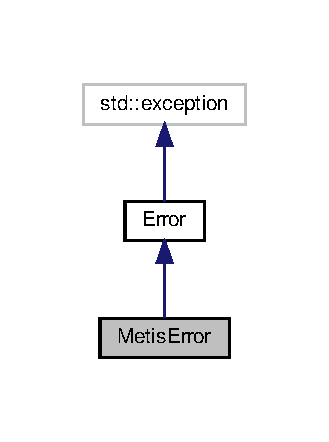
\includegraphics[width=158pt]{classMetisError__coll__graph}
\end{center}
\end{figure}
\subsection*{Public Member Functions}
\begin{DoxyCompactItemize}
\item 
\hyperlink{classMetisError_ac75e70bca56efa9b432897dba8e59fda}{Metis\+Error} (const std\+::string \&file, int line, const std\+::string \&func, int error\+\_\+code)
\begin{DoxyCompactList}\small\item\em Initializes a M\+E\+T\+IS error. \end{DoxyCompactList}\end{DoxyCompactItemize}


\subsection{Detailed Description}
\hyperlink{classMetisError}{Metis\+Error} is thrown when a M\+E\+T\+IS routine throws a non-\/zero error code. 

\subsection{Constructor \& Destructor Documentation}
\mbox{\Hypertarget{classMetisError_ac75e70bca56efa9b432897dba8e59fda}\label{classMetisError_ac75e70bca56efa9b432897dba8e59fda}} 
\index{Metis\+Error@{Metis\+Error}!Metis\+Error@{Metis\+Error}}
\index{Metis\+Error@{Metis\+Error}!Metis\+Error@{Metis\+Error}}
\subsubsection{\texorpdfstring{Metis\+Error()}{MetisError()}}
{\footnotesize\ttfamily Metis\+Error\+::\+Metis\+Error (\begin{DoxyParamCaption}\item[{const std\+::string \&}]{file,  }\item[{int}]{line,  }\item[{const std\+::string \&}]{func,  }\item[{int}]{error\+\_\+code }\end{DoxyParamCaption})\hspace{0.3cm}{\ttfamily [inline]}}



Initializes a M\+E\+T\+IS error. 


\begin{DoxyParams}{Parameters}
{\em file} & The name of the offending source file \\
\hline
{\em line} & The source code line number where the error occurred \\
\hline
{\em func} & The name of the M\+E\+T\+IS routine that failed \\
\hline
{\em error\+\_\+code} & The resulting M\+E\+T\+IS error code \\
\hline
\end{DoxyParams}


The documentation for this class was generated from the following files\+:\begin{DoxyCompactItemize}
\item 
exception.\+hpp (f54e8c2)\item 
/home/runner/work/schwarz-\/lib/schwarz-\/lib/source/exception.\+cpp (f54e8c2)\end{DoxyCompactItemize}

\hypertarget{classModuleNotImplemented}{}\section{Module\+Not\+Implemented Class Reference}
\label{classModuleNotImplemented}\index{Module\+Not\+Implemented@{Module\+Not\+Implemented}}


Collaboration diagram for Module\+Not\+Implemented\+:
\nopagebreak
\begin{figure}[H]
\begin{center}
\leavevmode
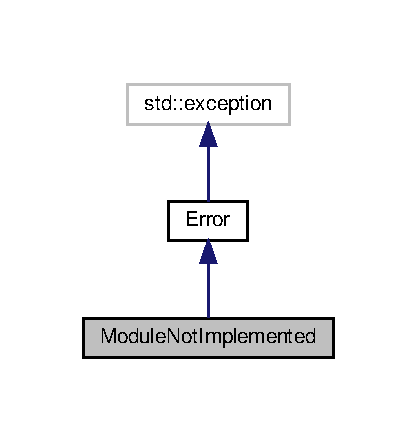
\includegraphics[width=200pt]{classModuleNotImplemented__coll__graph}
\end{center}
\end{figure}
\subsection*{Public Member Functions}
\begin{DoxyCompactItemize}
\item 
\hyperlink{classModuleNotImplemented_adf169bb339dbebbd025eda534d58fd6f}{Module\+Not\+Implemented} (const std\+::string \&file, int line, const std\+::string \&module, const std\+::string \&func)
\begin{DoxyCompactList}\small\item\em Initializes a \hyperlink{classNotImplemented}{Not\+Implemented} error. \end{DoxyCompactList}\end{DoxyCompactItemize}


\subsection{Constructor \& Destructor Documentation}
\mbox{\Hypertarget{classModuleNotImplemented_adf169bb339dbebbd025eda534d58fd6f}\label{classModuleNotImplemented_adf169bb339dbebbd025eda534d58fd6f}} 
\index{Module\+Not\+Implemented@{Module\+Not\+Implemented}!Module\+Not\+Implemented@{Module\+Not\+Implemented}}
\index{Module\+Not\+Implemented@{Module\+Not\+Implemented}!Module\+Not\+Implemented@{Module\+Not\+Implemented}}
\subsubsection{\texorpdfstring{Module\+Not\+Implemented()}{ModuleNotImplemented()}}
{\footnotesize\ttfamily Module\+Not\+Implemented\+::\+Module\+Not\+Implemented (\begin{DoxyParamCaption}\item[{const std\+::string \&}]{file,  }\item[{int}]{line,  }\item[{const std\+::string \&}]{module,  }\item[{const std\+::string \&}]{func }\end{DoxyParamCaption})\hspace{0.3cm}{\ttfamily [inline]}}



Initializes a \hyperlink{classNotImplemented}{Not\+Implemented} error. 


\begin{DoxyParams}{Parameters}
{\em file} & The name of the offending source file \\
\hline
{\em line} & The source code line number where the error occurred \\
\hline
{\em module} & The name of the not-\/yet implemented module \\
\hline
{\em func} & The name of the not-\/yet implemented function \\
\hline
\end{DoxyParams}


The documentation for this class was generated from the following file\+:\begin{DoxyCompactItemize}
\item 
exception.\+hpp (10366ee)\end{DoxyCompactItemize}

\hypertarget{classNotImplemented}{}\section{Not\+Implemented Class Reference}
\label{classNotImplemented}\index{Not\+Implemented@{Not\+Implemented}}


Collaboration diagram for Not\+Implemented\+:
\nopagebreak
\begin{figure}[H]
\begin{center}
\leavevmode
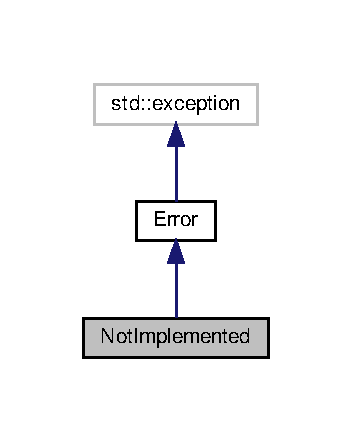
\includegraphics[width=169pt]{classNotImplemented__coll__graph}
\end{center}
\end{figure}
\subsection*{Public Member Functions}
\begin{DoxyCompactItemize}
\item 
\hyperlink{classNotImplemented_a744fb791ca16c8d500eaae24ec113aec}{Not\+Implemented} (const std\+::string \&file, int line, const std\+::string \&func)
\begin{DoxyCompactList}\small\item\em Initializes a \hyperlink{classNotImplemented}{Not\+Implemented} error. \end{DoxyCompactList}\end{DoxyCompactItemize}


\subsection{Constructor \& Destructor Documentation}
\mbox{\Hypertarget{classNotImplemented_a744fb791ca16c8d500eaae24ec113aec}\label{classNotImplemented_a744fb791ca16c8d500eaae24ec113aec}} 
\index{Not\+Implemented@{Not\+Implemented}!Not\+Implemented@{Not\+Implemented}}
\index{Not\+Implemented@{Not\+Implemented}!Not\+Implemented@{Not\+Implemented}}
\subsubsection{\texorpdfstring{Not\+Implemented()}{NotImplemented()}}
{\footnotesize\ttfamily Not\+Implemented\+::\+Not\+Implemented (\begin{DoxyParamCaption}\item[{const std\+::string \&}]{file,  }\item[{int}]{line,  }\item[{const std\+::string \&}]{func }\end{DoxyParamCaption})\hspace{0.3cm}{\ttfamily [inline]}}



Initializes a \hyperlink{classNotImplemented}{Not\+Implemented} error. 


\begin{DoxyParams}{Parameters}
{\em file} & The name of the offending source file \\
\hline
{\em line} & The source code line number where the error occurred \\
\hline
{\em func} & The name of the not-\/yet implemented function \\
\hline
\end{DoxyParams}


The documentation for this class was generated from the following file\+:\begin{DoxyCompactItemize}
\item 
exception.\+hpp (9a50ab9)\end{DoxyCompactItemize}

\hypertarget{structschwz_1_1Metadata_1_1post__process__data}{}\section{schwz\+:\+:Metadata$<$ Value\+Type, Index\+Type $>$\+:\+:post\+\_\+process\+\_\+data Struct Reference}
\label{structschwz_1_1Metadata_1_1post__process__data}\index{schwz\+::\+Metadata$<$ Value\+Type, Index\+Type $>$\+::post\+\_\+process\+\_\+data@{schwz\+::\+Metadata$<$ Value\+Type, Index\+Type $>$\+::post\+\_\+process\+\_\+data}}


The struct used for storing data for post-\/processing.  




{\ttfamily \#include $<$settings.\+hpp$>$}



Collaboration diagram for schwz\+:\+:Metadata$<$ Value\+Type, Index\+Type $>$\+:\+:post\+\_\+process\+\_\+data\+:
\nopagebreak
\begin{figure}[H]
\begin{center}
\leavevmode
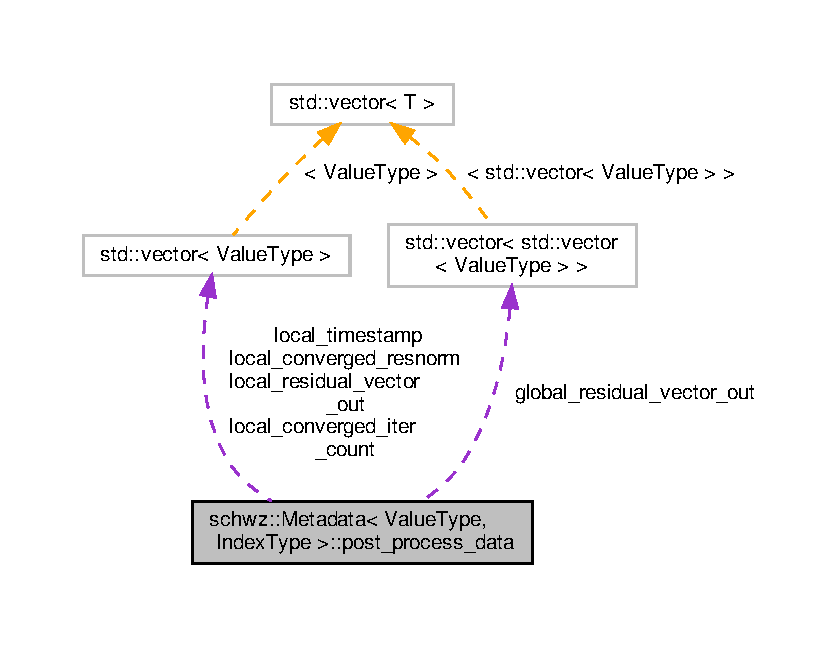
\includegraphics[width=350pt]{structschwz_1_1Metadata_1_1post__process__data__coll__graph}
\end{center}
\end{figure}
\subsection*{Public Attributes}
\begin{DoxyCompactItemize}
\item 
\mbox{\Hypertarget{structschwz_1_1Metadata_1_1post__process__data_a3cd4dc39548794213196924e925947e4}\label{structschwz_1_1Metadata_1_1post__process__data_a3cd4dc39548794213196924e925947e4}} 
std\+::vector$<$ std\+::vector$<$ Value\+Type $>$ $>$ {\bfseries global\+\_\+residual\+\_\+vector\+\_\+out}
\item 
\mbox{\Hypertarget{structschwz_1_1Metadata_1_1post__process__data_ac508dd9baaf55fe3eefaac84a081ea07}\label{structschwz_1_1Metadata_1_1post__process__data_ac508dd9baaf55fe3eefaac84a081ea07}} 
std\+::vector$<$ Value\+Type $>$ {\bfseries local\+\_\+residual\+\_\+vector\+\_\+out}
\item 
\mbox{\Hypertarget{structschwz_1_1Metadata_1_1post__process__data_ae089ea8c22e004373eb6f53c2db01383}\label{structschwz_1_1Metadata_1_1post__process__data_ae089ea8c22e004373eb6f53c2db01383}} 
std\+::vector$<$ Value\+Type $>$ {\bfseries local\+\_\+converged\+\_\+iter\+\_\+count}
\item 
\mbox{\Hypertarget{structschwz_1_1Metadata_1_1post__process__data_af03f16caf28849a9b1946c52d7d628fb}\label{structschwz_1_1Metadata_1_1post__process__data_af03f16caf28849a9b1946c52d7d628fb}} 
std\+::vector$<$ Value\+Type $>$ {\bfseries local\+\_\+converged\+\_\+resnorm}
\end{DoxyCompactItemize}


\subsection{Detailed Description}
\subsubsection*{template$<$typename Value\+Type, typename Index\+Type$>$\newline
struct schwz\+::\+Metadata$<$ Value\+Type, Index\+Type $>$\+::post\+\_\+process\+\_\+data}

The struct used for storing data for post-\/processing. 

The documentation for this struct was generated from the following file\+:\begin{DoxyCompactItemize}
\item 
settings.\+hpp (321b91c)\end{DoxyCompactItemize}

\hypertarget{structschwz_1_1Scatter}{}\section{schwz\+:\+:Scatter$<$ Value\+Type, Index\+Type $>$ Struct Template Reference}
\label{structschwz_1_1Scatter}\index{schwz\+::\+Scatter$<$ Value\+Type, Index\+Type $>$@{schwz\+::\+Scatter$<$ Value\+Type, Index\+Type $>$}}


Collaboration diagram for schwz\+:\+:Scatter$<$ Value\+Type, Index\+Type $>$\+:
\nopagebreak
\begin{figure}[H]
\begin{center}
\leavevmode
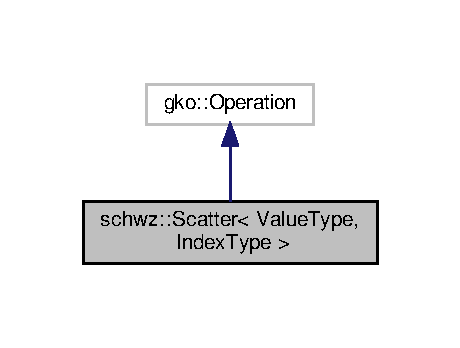
\includegraphics[width=221pt]{structschwz_1_1Scatter__coll__graph}
\end{center}
\end{figure}
\subsection*{Public Member Functions}
\begin{DoxyCompactItemize}
\item 
\mbox{\Hypertarget{structschwz_1_1Scatter_acf606095b1eb3546aa858a76ffe4b0e3}\label{structschwz_1_1Scatter_acf606095b1eb3546aa858a76ffe4b0e3}} 
{\bfseries Scatter} (const Index\+Type num\+\_\+elems, const Index\+Type $\ast$indices, const Value\+Type $\ast$from\+\_\+array, Value\+Type $\ast$into\+\_\+array, Operation\+Type optype)
\item 
\mbox{\Hypertarget{structschwz_1_1Scatter_a4887ae16bc4abacf64366359ab9b6ef6}\label{structschwz_1_1Scatter_a4887ae16bc4abacf64366359ab9b6ef6}} 
void {\bfseries run} (std\+::shared\+\_\+ptr$<$ const gko\+::\+Omp\+Executor $>$) const override
\item 
\mbox{\Hypertarget{structschwz_1_1Scatter_a12807bf0b409347b9a5e7c948b93be32}\label{structschwz_1_1Scatter_a12807bf0b409347b9a5e7c948b93be32}} 
void {\bfseries run} (std\+::shared\+\_\+ptr$<$ const gko\+::\+Cuda\+Executor $>$) const override
\end{DoxyCompactItemize}
\subsection*{Public Attributes}
\begin{DoxyCompactItemize}
\item 
\mbox{\Hypertarget{structschwz_1_1Scatter_a43252cdb86c252b755384ce913530016}\label{structschwz_1_1Scatter_a43252cdb86c252b755384ce913530016}} 
const Index\+Type {\bfseries num\+\_\+elems}
\item 
\mbox{\Hypertarget{structschwz_1_1Scatter_ace6df48951fb83fde6e7a69779253d8b}\label{structschwz_1_1Scatter_ace6df48951fb83fde6e7a69779253d8b}} 
const Index\+Type $\ast$ {\bfseries indices}
\item 
\mbox{\Hypertarget{structschwz_1_1Scatter_ad956399c31d1c016f97802de1b844440}\label{structschwz_1_1Scatter_ad956399c31d1c016f97802de1b844440}} 
const Value\+Type $\ast$ {\bfseries from\+\_\+array}
\item 
\mbox{\Hypertarget{structschwz_1_1Scatter_af0f17b144ec184891ad4f3411f6d83cc}\label{structschwz_1_1Scatter_af0f17b144ec184891ad4f3411f6d83cc}} 
Value\+Type $\ast$ {\bfseries into\+\_\+array}
\item 
\mbox{\Hypertarget{structschwz_1_1Scatter_a86486db4091ef57dc8e4526f1b9e8d94}\label{structschwz_1_1Scatter_a86486db4091ef57dc8e4526f1b9e8d94}} 
Operation\+Type {\bfseries optype}
\end{DoxyCompactItemize}


The documentation for this struct was generated from the following file\+:\begin{DoxyCompactItemize}
\item 
scatter.\+hpp (9d4939f)\end{DoxyCompactItemize}

\hypertarget{classschwz_1_1SchwarzBase}{}\section{schwz\+:\+:Schwarz\+Base$<$ Value\+Type, Index\+Type $>$ Class Template Reference}
\label{classschwz_1_1SchwarzBase}\index{schwz\+::\+Schwarz\+Base$<$ Value\+Type, Index\+Type $>$@{schwz\+::\+Schwarz\+Base$<$ Value\+Type, Index\+Type $>$}}


The Base solver class is meant to be the class implementing the common implementations for all the schwarz methods.  




{\ttfamily \#include $<$schwarz\+\_\+base.\+hpp$>$}



Collaboration diagram for schwz\+:\+:Schwarz\+Base$<$ Value\+Type, Index\+Type $>$\+:
\nopagebreak
\begin{figure}[H]
\begin{center}
\leavevmode
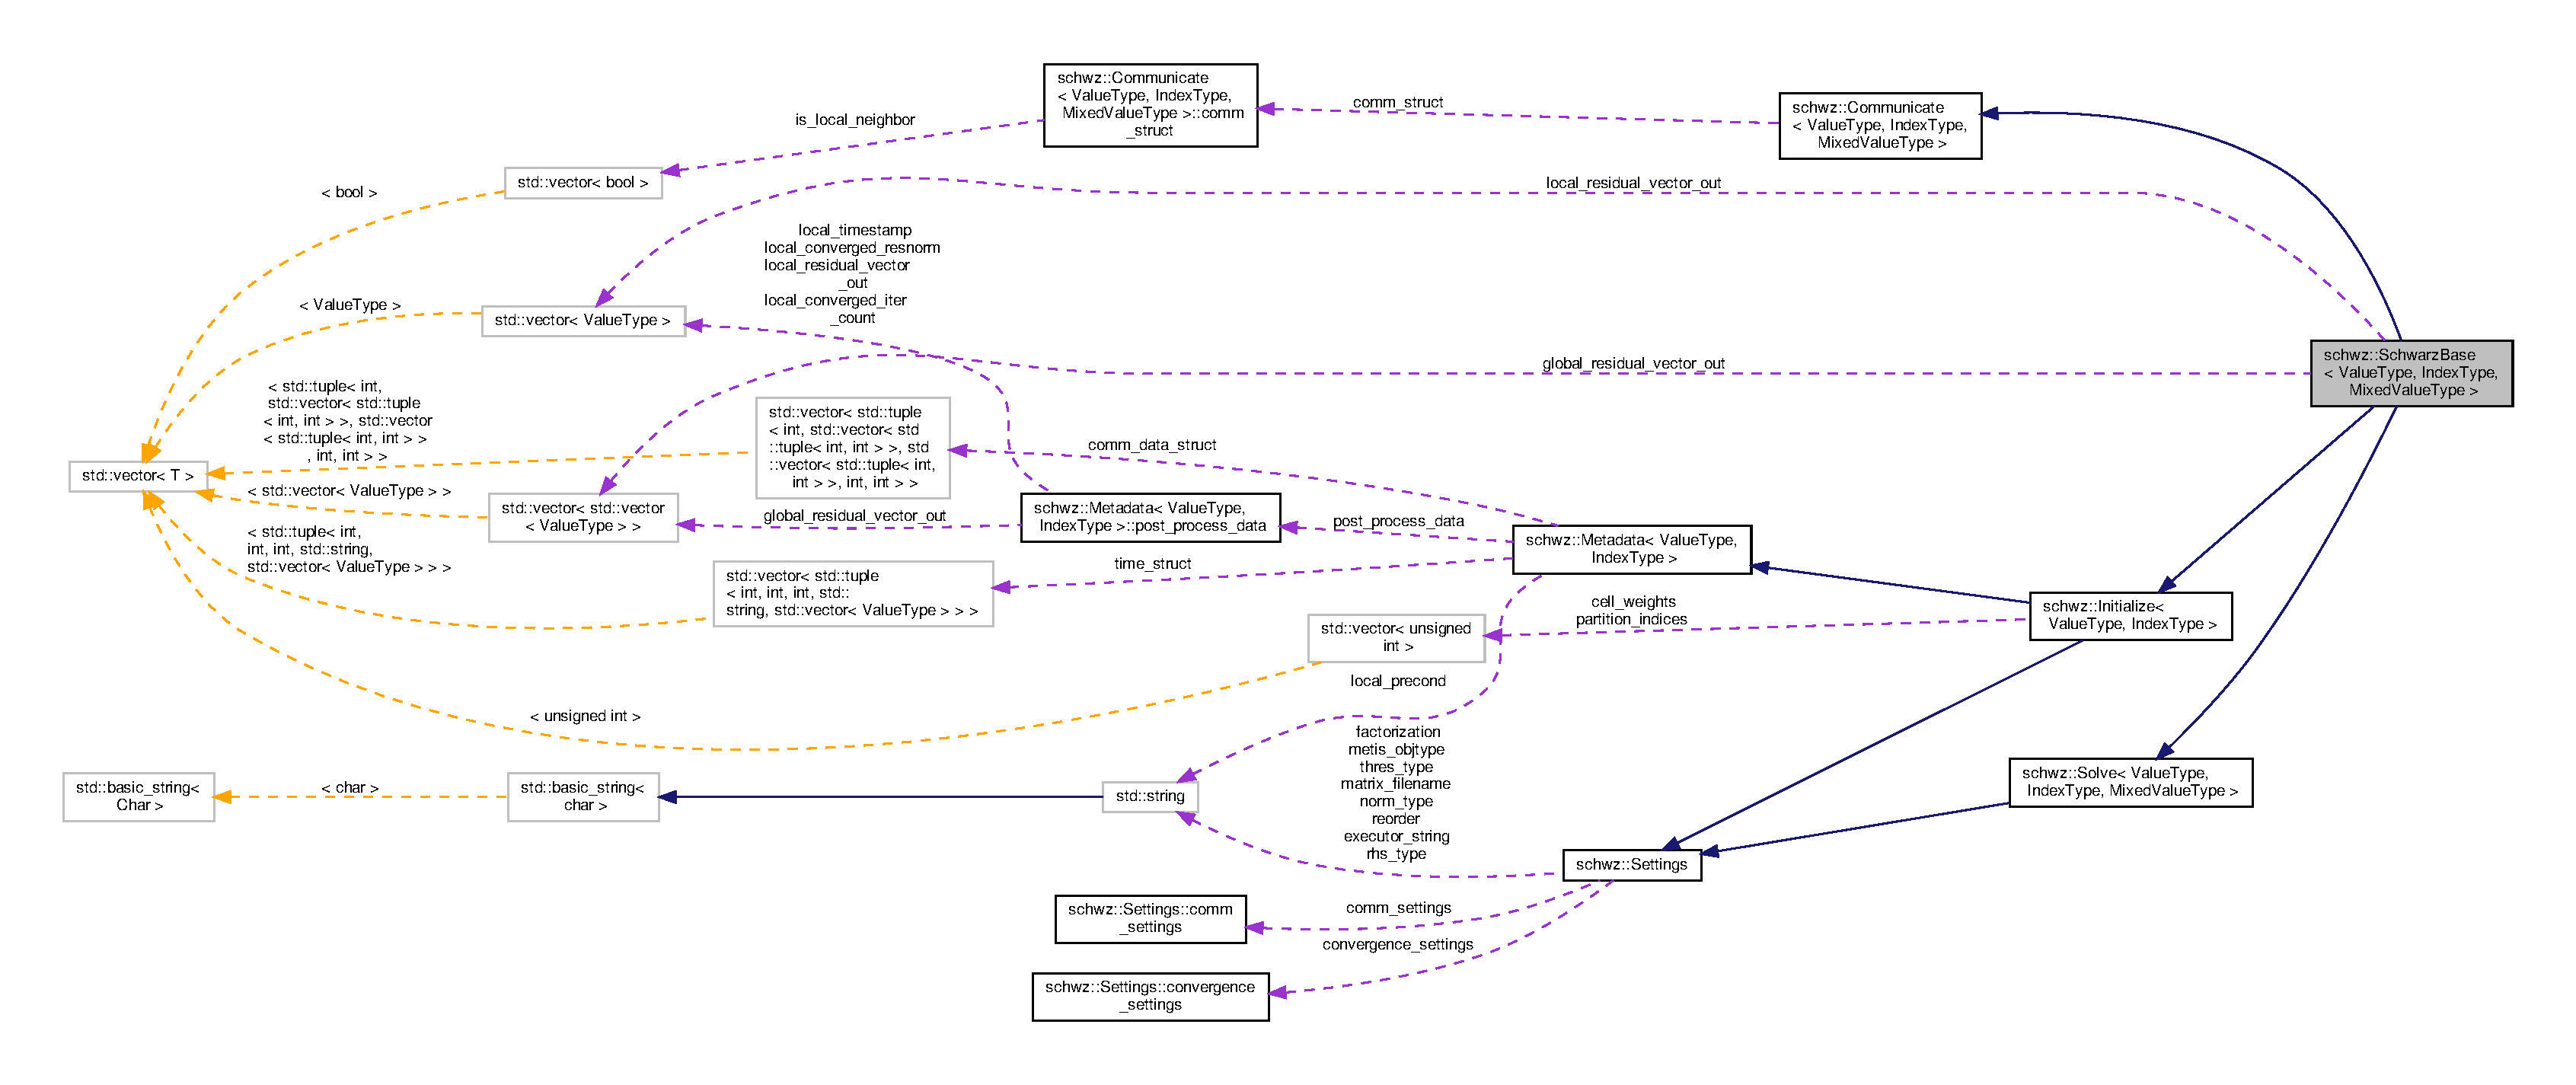
\includegraphics[width=350pt]{classschwz_1_1SchwarzBase__coll__graph}
\end{center}
\end{figure}
\subsection*{Public Member Functions}
\begin{DoxyCompactItemize}
\item 
\hyperlink{classschwz_1_1SchwarzBase_ab746eb6bb1c40d110ebd03cef0ddb415}{Schwarz\+Base} (\hyperlink{structschwz_1_1Settings}{Settings} \&settings, \hyperlink{structschwz_1_1Metadata}{Metadata}$<$ Value\+Type, Index\+Type $>$ \&metadata)
\begin{DoxyCompactList}\small\item\em The constructor that takes in the user settings and a metadata struct containing the solver metadata. \end{DoxyCompactList}\item 
\mbox{\Hypertarget{classschwz_1_1SchwarzBase_a276660ae87ca01cedce8846954b48d0f}\label{classschwz_1_1SchwarzBase_a276660ae87ca01cedce8846954b48d0f}} 
void \hyperlink{classschwz_1_1SchwarzBase_a276660ae87ca01cedce8846954b48d0f}{initialize} ()
\begin{DoxyCompactList}\small\item\em \hyperlink{classschwz_1_1Initialize}{Initialize} the matrix and vectors. \end{DoxyCompactList}\item 
void \hyperlink{classschwz_1_1SchwarzBase_ad4a01651b92f2bf44c4fedf8e1b9b33d}{run} (std\+::shared\+\_\+ptr$<$ gko\+::matrix\+::\+Dense$<$ Value\+Type $>$$>$ \&solution)
\begin{DoxyCompactList}\small\item\em The function that runs the actual solver and obtains the final solution. \end{DoxyCompactList}\item 
void \hyperlink{classschwz_1_1SchwarzBase_a432e5a033a82c5153dda2170ceb4a199}{print\+\_\+vector} (const std\+::shared\+\_\+ptr$<$ gko\+::matrix\+::\+Dense$<$ Value\+Type $>$$>$ \&vector, int subd, std\+::string name)
\begin{DoxyCompactList}\small\item\em The auxiliary function that prints a passed in vector. \end{DoxyCompactList}\item 
void \hyperlink{classschwz_1_1SchwarzBase_ae671d00ba78877589cb082724c469ff6}{print\+\_\+matrix} (const std\+::shared\+\_\+ptr$<$ gko\+::matrix\+::\+Csr$<$ Value\+Type, Index\+Type $>$$>$ \&matrix, int rank, std\+::string name)
\begin{DoxyCompactList}\small\item\em The auxiliary function that prints a passed in C\+SR matrix. \end{DoxyCompactList}\end{DoxyCompactItemize}
\subsection*{Public Attributes}
\begin{DoxyCompactItemize}
\item 
\mbox{\Hypertarget{classschwz_1_1SchwarzBase_a64bdd55bbab23c6e21d0621cd84a299b}\label{classschwz_1_1SchwarzBase_a64bdd55bbab23c6e21d0621cd84a299b}} 
std\+::shared\+\_\+ptr$<$ gko\+::matrix\+::\+Csr$<$ Value\+Type, Index\+Type $>$ $>$ \hyperlink{classschwz_1_1SchwarzBase_a64bdd55bbab23c6e21d0621cd84a299b}{local\+\_\+matrix}
\begin{DoxyCompactList}\small\item\em The local subdomain matrix. \end{DoxyCompactList}\item 
\mbox{\Hypertarget{classschwz_1_1SchwarzBase_abd75e7b8624c8a4b6f364f143e9cea17}\label{classschwz_1_1SchwarzBase_abd75e7b8624c8a4b6f364f143e9cea17}} 
std\+::shared\+\_\+ptr$<$ gko\+::matrix\+::\+Permutation$<$ Index\+Type $>$ $>$ \hyperlink{classschwz_1_1SchwarzBase_abd75e7b8624c8a4b6f364f143e9cea17}{local\+\_\+perm}
\begin{DoxyCompactList}\small\item\em The local subdomain permutation matrix/array. \end{DoxyCompactList}\item 
\mbox{\Hypertarget{classschwz_1_1SchwarzBase_af126dde2a173950bfc320ade7e26170b}\label{classschwz_1_1SchwarzBase_af126dde2a173950bfc320ade7e26170b}} 
std\+::shared\+\_\+ptr$<$ gko\+::matrix\+::\+Permutation$<$ Index\+Type $>$ $>$ \hyperlink{classschwz_1_1SchwarzBase_af126dde2a173950bfc320ade7e26170b}{local\+\_\+inv\+\_\+perm}
\begin{DoxyCompactList}\small\item\em The local subdomain inverse permutation matrix/array. \end{DoxyCompactList}\item 
\mbox{\Hypertarget{classschwz_1_1SchwarzBase_ab69b039ef8d83be1c05136ada846a766}\label{classschwz_1_1SchwarzBase_ab69b039ef8d83be1c05136ada846a766}} 
std\+::shared\+\_\+ptr$<$ gko\+::matrix\+::\+Csr$<$ Value\+Type, Index\+Type $>$ $>$ \hyperlink{classschwz_1_1SchwarzBase_ab69b039ef8d83be1c05136ada846a766}{triangular\+\_\+factor\+\_\+l}
\begin{DoxyCompactList}\small\item\em The local lower triangular factor used for the triangular solves. \end{DoxyCompactList}\item 
\mbox{\Hypertarget{classschwz_1_1SchwarzBase_adfb4459647e875717ea8812859f09fea}\label{classschwz_1_1SchwarzBase_adfb4459647e875717ea8812859f09fea}} 
std\+::shared\+\_\+ptr$<$ gko\+::matrix\+::\+Csr$<$ Value\+Type, Index\+Type $>$ $>$ \hyperlink{classschwz_1_1SchwarzBase_adfb4459647e875717ea8812859f09fea}{triangular\+\_\+factor\+\_\+u}
\begin{DoxyCompactList}\small\item\em The local upper triangular factor used for the triangular solves. \end{DoxyCompactList}\item 
\mbox{\Hypertarget{classschwz_1_1SchwarzBase_a1e9742522b50a7bebe936b6540694f72}\label{classschwz_1_1SchwarzBase_a1e9742522b50a7bebe936b6540694f72}} 
std\+::shared\+\_\+ptr$<$ gko\+::matrix\+::\+Csr$<$ Value\+Type, Index\+Type $>$ $>$ \hyperlink{classschwz_1_1SchwarzBase_a1e9742522b50a7bebe936b6540694f72}{interface\+\_\+matrix}
\begin{DoxyCompactList}\small\item\em The local interface matrix. \end{DoxyCompactList}\item 
\mbox{\Hypertarget{classschwz_1_1SchwarzBase_a3539b68fb6ff07a8f58b1f990976dc90}\label{classschwz_1_1SchwarzBase_a3539b68fb6ff07a8f58b1f990976dc90}} 
std\+::shared\+\_\+ptr$<$ gko\+::matrix\+::\+Csr$<$ Value\+Type, Index\+Type $>$ $>$ \hyperlink{classschwz_1_1SchwarzBase_a3539b68fb6ff07a8f58b1f990976dc90}{global\+\_\+matrix}
\begin{DoxyCompactList}\small\item\em The global matrix. \end{DoxyCompactList}\item 
\mbox{\Hypertarget{classschwz_1_1SchwarzBase_ac28b3e811e6016f31836fe366ff56eb7}\label{classschwz_1_1SchwarzBase_ac28b3e811e6016f31836fe366ff56eb7}} 
std\+::shared\+\_\+ptr$<$ gko\+::matrix\+::\+Dense$<$ Value\+Type $>$ $>$ \hyperlink{classschwz_1_1SchwarzBase_ac28b3e811e6016f31836fe366ff56eb7}{local\+\_\+rhs}
\begin{DoxyCompactList}\small\item\em The local right hand side. \end{DoxyCompactList}\item 
\mbox{\Hypertarget{classschwz_1_1SchwarzBase_a1a6313c3ce53d7868a1b87b807f1a1ce}\label{classschwz_1_1SchwarzBase_a1a6313c3ce53d7868a1b87b807f1a1ce}} 
std\+::shared\+\_\+ptr$<$ gko\+::matrix\+::\+Dense$<$ Value\+Type $>$ $>$ \hyperlink{classschwz_1_1SchwarzBase_a1a6313c3ce53d7868a1b87b807f1a1ce}{global\+\_\+rhs}
\begin{DoxyCompactList}\small\item\em The global right hand side. \end{DoxyCompactList}\item 
\mbox{\Hypertarget{classschwz_1_1SchwarzBase_a29ef68da307b6de9b8ae878df8fb19d4}\label{classschwz_1_1SchwarzBase_a29ef68da307b6de9b8ae878df8fb19d4}} 
std\+::shared\+\_\+ptr$<$ gko\+::matrix\+::\+Dense$<$ Value\+Type $>$ $>$ \hyperlink{classschwz_1_1SchwarzBase_a29ef68da307b6de9b8ae878df8fb19d4}{local\+\_\+solution}
\begin{DoxyCompactList}\small\item\em The local solution vector. \end{DoxyCompactList}\item 
\mbox{\Hypertarget{classschwz_1_1SchwarzBase_a8e6f088b8a7112af2ce27285d8d91bcc}\label{classschwz_1_1SchwarzBase_a8e6f088b8a7112af2ce27285d8d91bcc}} 
std\+::shared\+\_\+ptr$<$ gko\+::matrix\+::\+Dense$<$ Value\+Type $>$ $>$ \hyperlink{classschwz_1_1SchwarzBase_a8e6f088b8a7112af2ce27285d8d91bcc}{global\+\_\+solution}
\begin{DoxyCompactList}\small\item\em The global solution vector. \end{DoxyCompactList}\item 
\mbox{\Hypertarget{classschwz_1_1SchwarzBase_a1ecd383f150abee6b3076338ecc5e783}\label{classschwz_1_1SchwarzBase_a1ecd383f150abee6b3076338ecc5e783}} 
std\+::vector$<$ Value\+Type $>$ \hyperlink{classschwz_1_1SchwarzBase_a1ecd383f150abee6b3076338ecc5e783}{local\+\_\+residual\+\_\+vector\+\_\+out}
\begin{DoxyCompactList}\small\item\em The global residual vector. \end{DoxyCompactList}\item 
\mbox{\Hypertarget{classschwz_1_1SchwarzBase_ae060fc8510ce947d893204693755dd97}\label{classschwz_1_1SchwarzBase_ae060fc8510ce947d893204693755dd97}} 
std\+::vector$<$ std\+::vector$<$ Value\+Type $>$ $>$ \hyperlink{classschwz_1_1SchwarzBase_ae060fc8510ce947d893204693755dd97}{global\+\_\+residual\+\_\+vector\+\_\+out}
\begin{DoxyCompactList}\small\item\em The local residual vector. \end{DoxyCompactList}\end{DoxyCompactItemize}
\subsection*{Additional Inherited Members}


\subsection{Detailed Description}
\subsubsection*{template$<$typename Value\+Type = gko\+::default\+\_\+precision, typename Index\+Type = gko\+::int32$>$\newline
class schwz\+::\+Schwarz\+Base$<$ Value\+Type, Index\+Type $>$}

The Base solver class is meant to be the class implementing the common implementations for all the schwarz methods. 

It derives from the Initialization class, the Communication class and the \hyperlink{classschwz_1_1Solve}{Solve} class all of which are templated.


\begin{DoxyTemplParams}{Template Parameters}
{\em Value\+Type} & The type of the floating point values. \\
\hline
{\em Index\+Type} & The type of the index type values. \\
\hline
\end{DoxyTemplParams}


\subsection{Constructor \& Destructor Documentation}
\mbox{\Hypertarget{classschwz_1_1SchwarzBase_ab746eb6bb1c40d110ebd03cef0ddb415}\label{classschwz_1_1SchwarzBase_ab746eb6bb1c40d110ebd03cef0ddb415}} 
\index{schwz\+::\+Schwarz\+Base@{schwz\+::\+Schwarz\+Base}!Schwarz\+Base@{Schwarz\+Base}}
\index{Schwarz\+Base@{Schwarz\+Base}!schwz\+::\+Schwarz\+Base@{schwz\+::\+Schwarz\+Base}}
\subsubsection{\texorpdfstring{Schwarz\+Base()}{SchwarzBase()}}
{\footnotesize\ttfamily template$<$typename Value\+Type , typename Index\+Type $>$ \\
\hyperlink{classschwz_1_1SchwarzBase}{schwz\+::\+Schwarz\+Base}$<$ Value\+Type, Index\+Type $>$\+::\hyperlink{classschwz_1_1SchwarzBase}{Schwarz\+Base} (\begin{DoxyParamCaption}\item[{\hyperlink{structschwz_1_1Settings}{Settings} \&}]{settings,  }\item[{\hyperlink{structschwz_1_1Metadata}{Metadata}$<$ Value\+Type, Index\+Type $>$ \&}]{metadata }\end{DoxyParamCaption})}



The constructor that takes in the user settings and a metadata struct containing the solver metadata. 


\begin{DoxyParams}{Parameters}
{\em settings} & The settings struct. \\
\hline
{\em metadata} & The metadata struct. \\
\hline
\end{DoxyParams}


References schwz\+::\+Settings\+::cuda\+\_\+device\+\_\+guard, schwz\+::\+Settings\+::executor, schwz\+::\+Settings\+::executor\+\_\+string, schwz\+::\+Metadata$<$ Value\+Type, Index\+Type $>$\+::local\+\_\+num\+\_\+procs, schwz\+::\+Metadata$<$ Value\+Type, Index\+Type $>$\+::mpi\+\_\+communicator, schwz\+::\+Metadata$<$ Value\+Type, Index\+Type $>$\+::my\+\_\+local\+\_\+rank, and schwz\+::\+Metadata$<$ Value\+Type, Index\+Type $>$\+::my\+\_\+rank.



\subsection{Member Function Documentation}
\mbox{\Hypertarget{classschwz_1_1SchwarzBase_ae671d00ba78877589cb082724c469ff6}\label{classschwz_1_1SchwarzBase_ae671d00ba78877589cb082724c469ff6}} 
\index{schwz\+::\+Schwarz\+Base@{schwz\+::\+Schwarz\+Base}!print\+\_\+matrix@{print\+\_\+matrix}}
\index{print\+\_\+matrix@{print\+\_\+matrix}!schwz\+::\+Schwarz\+Base@{schwz\+::\+Schwarz\+Base}}
\subsubsection{\texorpdfstring{print\+\_\+matrix()}{print\_matrix()}}
{\footnotesize\ttfamily template$<$typename Value\+Type  = gko\+::default\+\_\+precision, typename Index\+Type  = gko\+::int32$>$ \\
void \hyperlink{classschwz_1_1SchwarzBase}{schwz\+::\+Schwarz\+Base}$<$ Value\+Type, Index\+Type $>$\+::print\+\_\+matrix (\begin{DoxyParamCaption}\item[{const std\+::shared\+\_\+ptr$<$ gko\+::matrix\+::\+Csr$<$ Value\+Type, Index\+Type $>$$>$ \&}]{matrix,  }\item[{int}]{rank,  }\item[{std\+::string}]{name }\end{DoxyParamCaption})}



The auxiliary function that prints a passed in C\+SR matrix. 


\begin{DoxyParams}{Parameters}
{\em matrix} & The matrix to be printed. \\
\hline
{\em subd} & The subdomain on which the vector exists. \\
\hline
{\em name} & The name of the matrix as a string. \\
\hline
\end{DoxyParams}
\mbox{\Hypertarget{classschwz_1_1SchwarzBase_a432e5a033a82c5153dda2170ceb4a199}\label{classschwz_1_1SchwarzBase_a432e5a033a82c5153dda2170ceb4a199}} 
\index{schwz\+::\+Schwarz\+Base@{schwz\+::\+Schwarz\+Base}!print\+\_\+vector@{print\+\_\+vector}}
\index{print\+\_\+vector@{print\+\_\+vector}!schwz\+::\+Schwarz\+Base@{schwz\+::\+Schwarz\+Base}}
\subsubsection{\texorpdfstring{print\+\_\+vector()}{print\_vector()}}
{\footnotesize\ttfamily template$<$typename Value\+Type  = gko\+::default\+\_\+precision, typename Index\+Type  = gko\+::int32$>$ \\
void \hyperlink{classschwz_1_1SchwarzBase}{schwz\+::\+Schwarz\+Base}$<$ Value\+Type, Index\+Type $>$\+::print\+\_\+vector (\begin{DoxyParamCaption}\item[{const std\+::shared\+\_\+ptr$<$ gko\+::matrix\+::\+Dense$<$ Value\+Type $>$$>$ \&}]{vector,  }\item[{int}]{subd,  }\item[{std\+::string}]{name }\end{DoxyParamCaption})}



The auxiliary function that prints a passed in vector. 


\begin{DoxyParams}{Parameters}
{\em vector} & The vector to be printed. \\
\hline
{\em subd} & The subdomain on which the vector exists. \\
\hline
{\em name} & The name of the vector as a string. \\
\hline
\end{DoxyParams}
\mbox{\Hypertarget{classschwz_1_1SchwarzBase_ad4a01651b92f2bf44c4fedf8e1b9b33d}\label{classschwz_1_1SchwarzBase_ad4a01651b92f2bf44c4fedf8e1b9b33d}} 
\index{schwz\+::\+Schwarz\+Base@{schwz\+::\+Schwarz\+Base}!run@{run}}
\index{run@{run}!schwz\+::\+Schwarz\+Base@{schwz\+::\+Schwarz\+Base}}
\subsubsection{\texorpdfstring{run()}{run()}}
{\footnotesize\ttfamily template$<$typename Value\+Type , typename Index\+Type $>$ \\
void \hyperlink{classschwz_1_1SchwarzBase}{schwz\+::\+Schwarz\+Base}$<$ Value\+Type, Index\+Type $>$\+::run (\begin{DoxyParamCaption}\item[{std\+::shared\+\_\+ptr$<$ gko\+::matrix\+::\+Dense$<$ Value\+Type $>$$>$ \&}]{solution }\end{DoxyParamCaption})}



The function that runs the actual solver and obtains the final solution. 


\begin{DoxyParams}{Parameters}
{\em solution} & The solution vector. \\
\hline
\end{DoxyParams}


References schwz\+::\+Communicate$<$ Value\+Type, Index\+Type $>$\+::exchange\+\_\+boundary(), schwz\+::\+Settings\+::executor, schwz\+::\+Schwarz\+Base$<$ Value\+Type, Index\+Type $>$\+::global\+\_\+matrix, schwz\+::\+Schwarz\+Base$<$ Value\+Type, Index\+Type $>$\+::global\+\_\+rhs, schwz\+::\+Schwarz\+Base$<$ Value\+Type, Index\+Type $>$\+::global\+\_\+solution, schwz\+::\+Schwarz\+Base$<$ Value\+Type, Index\+Type $>$\+::interface\+\_\+matrix, schwz\+::\+Schwarz\+Base$<$ Value\+Type, Index\+Type $>$\+::local\+\_\+inv\+\_\+perm, schwz\+::\+Schwarz\+Base$<$ Value\+Type, Index\+Type $>$\+::local\+\_\+matrix, schwz\+::\+Schwarz\+Base$<$ Value\+Type, Index\+Type $>$\+::local\+\_\+perm, schwz\+::\+Schwarz\+Base$<$ Value\+Type, Index\+Type $>$\+::local\+\_\+rhs, schwz\+::\+Schwarz\+Base$<$ Value\+Type, Index\+Type $>$\+::local\+\_\+solution, schwz\+::\+Communicate$<$ Value\+Type, Index\+Type $>$\+::setup\+\_\+windows(), schwz\+::\+Schwarz\+Base$<$ Value\+Type, Index\+Type $>$\+::triangular\+\_\+factor\+\_\+l, schwz\+::\+Schwarz\+Base$<$ Value\+Type, Index\+Type $>$\+::triangular\+\_\+factor\+\_\+u, schwz\+::\+Communicate$<$ Value\+Type, Index\+Type $>$\+::update\+\_\+boundary(), and schwz\+::\+Settings\+::write\+\_\+iters\+\_\+and\+\_\+residuals.



The documentation for this class was generated from the following files\+:\begin{DoxyCompactItemize}
\item 
schwarz\+\_\+base.\+hpp (6b0b604)\item 
/home/runner/work/schwarz-\/lib/schwarz-\/lib/source/schwarz\+\_\+base.\+cpp (6b0b604)\end{DoxyCompactItemize}

\hypertarget{structschwz_1_1Settings}{}\section{schwz\+:\+:Settings Struct Reference}
\label{structschwz_1_1Settings}\index{schwz\+::\+Settings@{schwz\+::\+Settings}}


The struct that contains the solver settings and the parameters to be set by the user.  




{\ttfamily \#include $<$settings.\+hpp$>$}



Collaboration diagram for schwz\+:\+:Settings\+:
\nopagebreak
\begin{figure}[H]
\begin{center}
\leavevmode
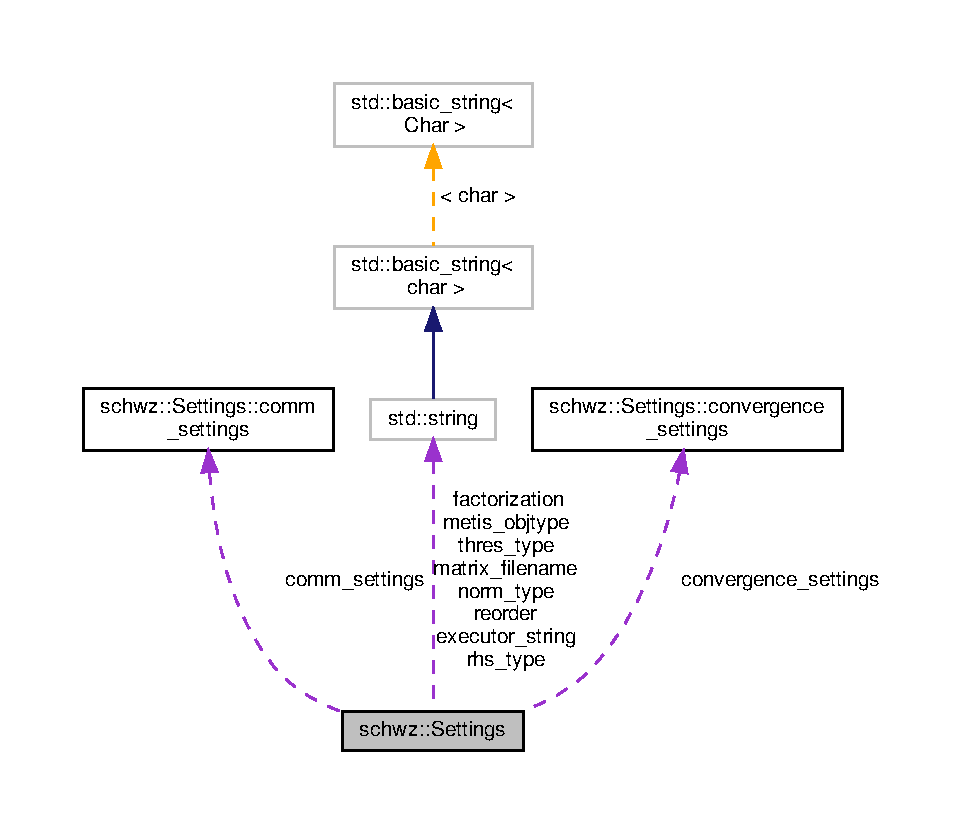
\includegraphics[width=350pt]{structschwz_1_1Settings__coll__graph}
\end{center}
\end{figure}
\subsection*{Classes}
\begin{DoxyCompactItemize}
\item 
struct \hyperlink{structschwz_1_1Settings_1_1comm__settings}{comm\+\_\+settings}
\begin{DoxyCompactList}\small\item\em The settings for the various available communication paradigms. \end{DoxyCompactList}\item 
struct \hyperlink{structschwz_1_1Settings_1_1convergence__settings}{convergence\+\_\+settings}
\begin{DoxyCompactList}\small\item\em The various convergence settings available. \end{DoxyCompactList}\end{DoxyCompactItemize}
\subsection*{Public Types}
\begin{DoxyCompactItemize}
\item 
\mbox{\Hypertarget{structschwz_1_1Settings_a11769093e4aa3ce3340cbf7a67487faa}\label{structschwz_1_1Settings_a11769093e4aa3ce3340cbf7a67487faa}} 
enum \hyperlink{structschwz_1_1Settings_a11769093e4aa3ce3340cbf7a67487faa}{partition\+\_\+settings} \{ \newline
{\bfseries partition\+\_\+regular} = 0x0, 
{\bfseries partition\+\_\+regular2d} = 0x4, 
{\bfseries partition\+\_\+metis} = 0x1, 
{\bfseries partition\+\_\+zoltan} = 0x2, 
\newline
{\bfseries partition\+\_\+custom} = 0x3
 \}\begin{DoxyCompactList}\small\item\em The partition algorithm to be used for partitioning the matrix. \end{DoxyCompactList}
\item 
\mbox{\Hypertarget{structschwz_1_1Settings_a31e82310ef6aed08168baef78f0db69e}\label{structschwz_1_1Settings_a31e82310ef6aed08168baef78f0db69e}} 
enum \hyperlink{structschwz_1_1Settings_a31e82310ef6aed08168baef78f0db69e}{local\+\_\+solver\+\_\+settings} \{ \newline
{\bfseries direct\+\_\+solver\+\_\+cholmod} = 0x0, 
{\bfseries direct\+\_\+solver\+\_\+umfpack} = 0x5, 
{\bfseries direct\+\_\+solver\+\_\+ginkgo} = 0x1, 
{\bfseries iterative\+\_\+solver\+\_\+ginkgo} = 0x2, 
\newline
{\bfseries iterative\+\_\+solver\+\_\+dealii} = 0x3, 
{\bfseries solver\+\_\+custom} = 0x4
 \}\begin{DoxyCompactList}\small\item\em The local solver algorithm for the local subdomain solves. \end{DoxyCompactList}
\end{DoxyCompactItemize}
\subsection*{Public Member Functions}
\begin{DoxyCompactItemize}
\item 
\mbox{\Hypertarget{structschwz_1_1Settings_a00ac65d16e2ef2761fad0095b2ba3086}\label{structschwz_1_1Settings_a00ac65d16e2ef2761fad0095b2ba3086}} 
{\bfseries Settings} (std\+::string \hyperlink{structschwz_1_1Settings_a088ed3524456a1fd40e76b0e2d624c79}{executor\+\_\+string}=\char`\"{}reference\char`\"{})
\end{DoxyCompactItemize}
\subsection*{Public Attributes}
\begin{DoxyCompactItemize}
\item 
\mbox{\Hypertarget{structschwz_1_1Settings_a088ed3524456a1fd40e76b0e2d624c79}\label{structschwz_1_1Settings_a088ed3524456a1fd40e76b0e2d624c79}} 
std\+::string \hyperlink{structschwz_1_1Settings_a088ed3524456a1fd40e76b0e2d624c79}{executor\+\_\+string}
\begin{DoxyCompactList}\small\item\em The string that contains the ginkgo executor paradigm. \end{DoxyCompactList}\item 
\mbox{\Hypertarget{structschwz_1_1Settings_a6920db9b39120b83399743083f17691f}\label{structschwz_1_1Settings_a6920db9b39120b83399743083f17691f}} 
std\+::shared\+\_\+ptr$<$ gko\+::\+Executor $>$ \hyperlink{structschwz_1_1Settings_a6920db9b39120b83399743083f17691f}{executor} = gko\+::\+Reference\+Executor\+::create()
\begin{DoxyCompactList}\small\item\em The ginkgo executor the code is to be executed on. \end{DoxyCompactList}\item 
\mbox{\Hypertarget{structschwz_1_1Settings_ae32b9a9c03095a47810aa2fc0915eec7}\label{structschwz_1_1Settings_ae32b9a9c03095a47810aa2fc0915eec7}} 
std\+::shared\+\_\+ptr$<$ \hyperlink{classschwz_1_1device__guard}{device\+\_\+guard} $>$ \hyperlink{structschwz_1_1Settings_ae32b9a9c03095a47810aa2fc0915eec7}{cuda\+\_\+device\+\_\+guard}
\begin{DoxyCompactList}\small\item\em The ginkgo executor the code is to be executed on. \end{DoxyCompactList}\item 
\mbox{\Hypertarget{structschwz_1_1Settings_ac1e336d221bc2238a5e020900d7ae4c8}\label{structschwz_1_1Settings_ac1e336d221bc2238a5e020900d7ae4c8}} 
\hyperlink{structschwz_1_1Settings_a11769093e4aa3ce3340cbf7a67487faa}{partition\+\_\+settings} {\bfseries partition} = partition\+\_\+settings\+::partition\+\_\+regular
\item 
\mbox{\Hypertarget{structschwz_1_1Settings_acf1f443835c2ac601782827f512bdd05}\label{structschwz_1_1Settings_acf1f443835c2ac601782827f512bdd05}} 
gko\+::int32 \hyperlink{structschwz_1_1Settings_acf1f443835c2ac601782827f512bdd05}{overlap} = 2
\begin{DoxyCompactList}\small\item\em The overlap between the subdomains. \end{DoxyCompactList}\item 
\mbox{\Hypertarget{structschwz_1_1Settings_a30bee3efa70fac8650d1c2837f1ba9c8}\label{structschwz_1_1Settings_a30bee3efa70fac8650d1c2837f1ba9c8}} 
std\+::string \hyperlink{structschwz_1_1Settings_a30bee3efa70fac8650d1c2837f1ba9c8}{matrix\+\_\+filename} = \char`\"{}null\char`\"{}
\begin{DoxyCompactList}\small\item\em The string that contains the matrix file name to read from . \end{DoxyCompactList}\item 
bool \hyperlink{structschwz_1_1Settings_a2af5f07901df047e305c456b2f97e774}{explicit\+\_\+laplacian} = true
\begin{DoxyCompactList}\small\item\em Flag if the laplacian matrix should be generated within the library. \end{DoxyCompactList}\item 
\mbox{\Hypertarget{structschwz_1_1Settings_a1bb8b8ee875222bd73899ebf0447fa4e}\label{structschwz_1_1Settings_a1bb8b8ee875222bd73899ebf0447fa4e}} 
bool \hyperlink{structschwz_1_1Settings_a1bb8b8ee875222bd73899ebf0447fa4e}{use\+\_\+mixed\+\_\+precision} = false
\begin{DoxyCompactList}\small\item\em Flag if mixed precision should be used. \end{DoxyCompactList}\item 
\mbox{\Hypertarget{structschwz_1_1Settings_a04760b39513414af70498808c0a6b317}\label{structschwz_1_1Settings_a04760b39513414af70498808c0a6b317}} 
bool \hyperlink{structschwz_1_1Settings_a04760b39513414af70498808c0a6b317}{enable\+\_\+random\+\_\+rhs} = false
\begin{DoxyCompactList}\small\item\em Flag to enable a random rhs. \end{DoxyCompactList}\item 
\mbox{\Hypertarget{structschwz_1_1Settings_afdf517a873a887a21a03b75c1011f903}\label{structschwz_1_1Settings_afdf517a873a887a21a03b75c1011f903}} 
bool \hyperlink{structschwz_1_1Settings_afdf517a873a887a21a03b75c1011f903}{print\+\_\+matrices} = false
\begin{DoxyCompactList}\small\item\em Flag to enable printing of matrices. \end{DoxyCompactList}\item 
\mbox{\Hypertarget{structschwz_1_1Settings_a5573fab398e7bba73e793eea06aa1e11}\label{structschwz_1_1Settings_a5573fab398e7bba73e793eea06aa1e11}} 
bool \hyperlink{structschwz_1_1Settings_a5573fab398e7bba73e793eea06aa1e11}{debug\+\_\+print} = false
\begin{DoxyCompactList}\small\item\em Flag to enable some debug printing. \end{DoxyCompactList}\item 
\hyperlink{structschwz_1_1Settings_a31e82310ef6aed08168baef78f0db69e}{local\+\_\+solver\+\_\+settings} {\bfseries local\+\_\+solver}
\item 
\mbox{\Hypertarget{structschwz_1_1Settings_a5f110676f929eebeb357cb07398e2048}\label{structschwz_1_1Settings_a5f110676f929eebeb357cb07398e2048}} 
bool \hyperlink{structschwz_1_1Settings_a5f110676f929eebeb357cb07398e2048}{non\+\_\+symmetric\+\_\+matrix} = false
\begin{DoxyCompactList}\small\item\em Is the matrix non-\/symmetric ? , Use G\+M\+R\+ES for local solves. \end{DoxyCompactList}\item 
\mbox{\Hypertarget{structschwz_1_1Settings_a7d26302ccb58fd96c795046ecc577694}\label{structschwz_1_1Settings_a7d26302ccb58fd96c795046ecc577694}} 
unsigned int \hyperlink{structschwz_1_1Settings_a7d26302ccb58fd96c795046ecc577694}{restart\+\_\+iter} = 1u
\begin{DoxyCompactList}\small\item\em The restart iter for the G\+M\+R\+ES solver. \end{DoxyCompactList}\item 
\mbox{\Hypertarget{structschwz_1_1Settings_af257396850c46e4d3217b4bb1a858114}\label{structschwz_1_1Settings_af257396850c46e4d3217b4bb1a858114}} 
int \hyperlink{structschwz_1_1Settings_af257396850c46e4d3217b4bb1a858114}{reset\+\_\+local\+\_\+crit\+\_\+iter} = -\/1
\begin{DoxyCompactList}\small\item\em The global iter at which to reset the local solver criterion. \end{DoxyCompactList}\item 
bool \hyperlink{structschwz_1_1Settings_a75a2ff3778c7334382a6c74553dbd5b4}{naturally\+\_\+ordered\+\_\+factor} = false
\begin{DoxyCompactList}\small\item\em Disables the re-\/ordering of the matrix before computing the triangular factors during the C\+H\+O\+L\+M\+OD factorization. \end{DoxyCompactList}\item 
\mbox{\Hypertarget{structschwz_1_1Settings_a8a057e4ac5331c9222ad539ffd1f5c3d}\label{structschwz_1_1Settings_a8a057e4ac5331c9222ad539ffd1f5c3d}} 
std\+::string \hyperlink{structschwz_1_1Settings_a8a057e4ac5331c9222ad539ffd1f5c3d}{metis\+\_\+objtype}
\begin{DoxyCompactList}\small\item\em This setting defines the objective type for the metis partitioning. \end{DoxyCompactList}\item 
\mbox{\Hypertarget{structschwz_1_1Settings_ab51cf8eda75e05280084e89895121ca7}\label{structschwz_1_1Settings_ab51cf8eda75e05280084e89895121ca7}} 
bool \hyperlink{structschwz_1_1Settings_ab51cf8eda75e05280084e89895121ca7}{use\+\_\+precond} = false
\begin{DoxyCompactList}\small\item\em Enable the block jacobi local preconditioner for the local solver. \end{DoxyCompactList}\item 
\mbox{\Hypertarget{structschwz_1_1Settings_af81ff061a4d7220d380fb7f579d7a6e1}\label{structschwz_1_1Settings_af81ff061a4d7220d380fb7f579d7a6e1}} 
bool \hyperlink{structschwz_1_1Settings_af81ff061a4d7220d380fb7f579d7a6e1}{write\+\_\+debug\+\_\+out} = false
\begin{DoxyCompactList}\small\item\em Enable the writing of debug out to file. \end{DoxyCompactList}\item 
\mbox{\Hypertarget{structschwz_1_1Settings_a5555cf4340e7918ce22d00b26ccca6a7}\label{structschwz_1_1Settings_a5555cf4340e7918ce22d00b26ccca6a7}} 
bool \hyperlink{structschwz_1_1Settings_a5555cf4340e7918ce22d00b26ccca6a7}{write\+\_\+iters\+\_\+and\+\_\+residuals} = false
\begin{DoxyCompactList}\small\item\em Enable writing the iters and residuals to a file. \end{DoxyCompactList}\item 
bool \hyperlink{structschwz_1_1Settings_a2b683340720aadaba85255580483f684}{enable\+\_\+logging} = false
\begin{DoxyCompactList}\small\item\em Flag to enable logging for local iterative solvers. \end{DoxyCompactList}\item 
\mbox{\Hypertarget{structschwz_1_1Settings_af692ca8550d16b538dcfddb5208e73f3}\label{structschwz_1_1Settings_af692ca8550d16b538dcfddb5208e73f3}} 
bool \hyperlink{structschwz_1_1Settings_af692ca8550d16b538dcfddb5208e73f3}{write\+\_\+perm\+\_\+data} = false
\begin{DoxyCompactList}\small\item\em Enable the local permutations from C\+H\+O\+L\+M\+OD to a file. \end{DoxyCompactList}\item 
\mbox{\Hypertarget{structschwz_1_1Settings_a33a9382f1b5961a8cb2133cb0c22daf0}\label{structschwz_1_1Settings_a33a9382f1b5961a8cb2133cb0c22daf0}} 
int \hyperlink{structschwz_1_1Settings_a33a9382f1b5961a8cb2133cb0c22daf0}{shifted\+\_\+iter} = 1
\begin{DoxyCompactList}\small\item\em Iteration shift for node local communication. \end{DoxyCompactList}\item 
\mbox{\Hypertarget{structschwz_1_1Settings_a063efd688bb2442d72165d1cbb230fc6}\label{structschwz_1_1Settings_a063efd688bb2442d72165d1cbb230fc6}} 
\hyperlink{structschwz_1_1Settings_1_1comm__settings}{comm\+\_\+settings} {\bfseries comm\+\_\+settings}
\item 
\mbox{\Hypertarget{structschwz_1_1Settings_aba00c697bd92d6ed6332eaaf047c69a0}\label{structschwz_1_1Settings_aba00c697bd92d6ed6332eaaf047c69a0}} 
\hyperlink{structschwz_1_1Settings_1_1convergence__settings}{convergence\+\_\+settings} {\bfseries convergence\+\_\+settings}
\item 
\mbox{\Hypertarget{structschwz_1_1Settings_a9ac5443eff787613f4f39843cbfa568d}\label{structschwz_1_1Settings_a9ac5443eff787613f4f39843cbfa568d}} 
std\+::string \hyperlink{structschwz_1_1Settings_a9ac5443eff787613f4f39843cbfa568d}{factorization} = \char`\"{}cholmod\char`\"{}
\begin{DoxyCompactList}\small\item\em The factorization for the local direct solver. \end{DoxyCompactList}\item 
\mbox{\Hypertarget{structschwz_1_1Settings_a429197e8093f3f87664ee6c37f91068e}\label{structschwz_1_1Settings_a429197e8093f3f87664ee6c37f91068e}} 
std\+::string \hyperlink{structschwz_1_1Settings_a429197e8093f3f87664ee6c37f91068e}{reorder}
\begin{DoxyCompactList}\small\item\em The reordering for the local solve. \end{DoxyCompactList}\end{DoxyCompactItemize}


\subsection{Detailed Description}
The struct that contains the solver settings and the parameters to be set by the user. 

settings 

\subsection{Member Data Documentation}
\mbox{\Hypertarget{structschwz_1_1Settings_a2b683340720aadaba85255580483f684}\label{structschwz_1_1Settings_a2b683340720aadaba85255580483f684}} 
\index{schwz\+::\+Settings@{schwz\+::\+Settings}!enable\+\_\+logging@{enable\+\_\+logging}}
\index{enable\+\_\+logging@{enable\+\_\+logging}!schwz\+::\+Settings@{schwz\+::\+Settings}}
\subsubsection{\texorpdfstring{enable\+\_\+logging}{enable\_logging}}
{\footnotesize\ttfamily bool schwz\+::\+Settings\+::enable\+\_\+logging = false}



Flag to enable logging for local iterative solvers. 

Note\+: Probably will have a significant performance hit. \mbox{\Hypertarget{structschwz_1_1Settings_a2af5f07901df047e305c456b2f97e774}\label{structschwz_1_1Settings_a2af5f07901df047e305c456b2f97e774}} 
\index{schwz\+::\+Settings@{schwz\+::\+Settings}!explicit\+\_\+laplacian@{explicit\+\_\+laplacian}}
\index{explicit\+\_\+laplacian@{explicit\+\_\+laplacian}!schwz\+::\+Settings@{schwz\+::\+Settings}}
\subsubsection{\texorpdfstring{explicit\+\_\+laplacian}{explicit\_laplacian}}
{\footnotesize\ttfamily bool schwz\+::\+Settings\+::explicit\+\_\+laplacian = true}



Flag if the laplacian matrix should be generated within the library. 

If false, an external matrix and rhs needs to be provided 

Referenced by schwz\+::\+Schwarz\+Base$<$ Value\+Type, Index\+Type, Mixed\+Value\+Type $>$\+::initialize().

\mbox{\Hypertarget{structschwz_1_1Settings_a8028fcf029fadc07a7d1b9aa94c83f08}\label{structschwz_1_1Settings_a8028fcf029fadc07a7d1b9aa94c83f08}} 
\index{schwz\+::\+Settings@{schwz\+::\+Settings}!local\+\_\+solver@{local\+\_\+solver}}
\index{local\+\_\+solver@{local\+\_\+solver}!schwz\+::\+Settings@{schwz\+::\+Settings}}
\subsubsection{\texorpdfstring{local\+\_\+solver}{local\_solver}}
{\footnotesize\ttfamily \hyperlink{structschwz_1_1Settings_a31e82310ef6aed08168baef78f0db69e}{local\+\_\+solver\+\_\+settings} schwz\+::\+Settings\+::local\+\_\+solver}

{\bfseries Initial value\+:}
\begin{DoxyCode}
=
        local\_solver\_settings::iterative\_solver\_ginkgo
\end{DoxyCode}
\mbox{\Hypertarget{structschwz_1_1Settings_a75a2ff3778c7334382a6c74553dbd5b4}\label{structschwz_1_1Settings_a75a2ff3778c7334382a6c74553dbd5b4}} 
\index{schwz\+::\+Settings@{schwz\+::\+Settings}!naturally\+\_\+ordered\+\_\+factor@{naturally\+\_\+ordered\+\_\+factor}}
\index{naturally\+\_\+ordered\+\_\+factor@{naturally\+\_\+ordered\+\_\+factor}!schwz\+::\+Settings@{schwz\+::\+Settings}}
\subsubsection{\texorpdfstring{naturally\+\_\+ordered\+\_\+factor}{naturally\_ordered\_factor}}
{\footnotesize\ttfamily bool schwz\+::\+Settings\+::naturally\+\_\+ordered\+\_\+factor = false}



Disables the re-\/ordering of the matrix before computing the triangular factors during the C\+H\+O\+L\+M\+OD factorization. 

\begin{DoxyNote}{Note}
This is mainly to allow compatibility with G\+PU solution. 
\end{DoxyNote}


The documentation for this struct was generated from the following file\+:\begin{DoxyCompactItemize}
\item 
settings.\+hpp (522dfaf)\end{DoxyCompactItemize}

\hypertarget{classschwz_1_1Solve}{}\section{schwz\+:\+:Solve$<$ Value\+Type, Index\+Type $>$ Class Template Reference}
\label{classschwz_1_1Solve}\index{schwz\+::\+Solve$<$ Value\+Type, Index\+Type $>$@{schwz\+::\+Solve$<$ Value\+Type, Index\+Type $>$}}


The Solver class the provides the solver and the convergence checking methods.  




{\ttfamily \#include $<$solve.\+hpp$>$}



Collaboration diagram for schwz\+:\+:Solve$<$ Value\+Type, Index\+Type $>$\+:
\nopagebreak
\begin{figure}[H]
\begin{center}
\leavevmode
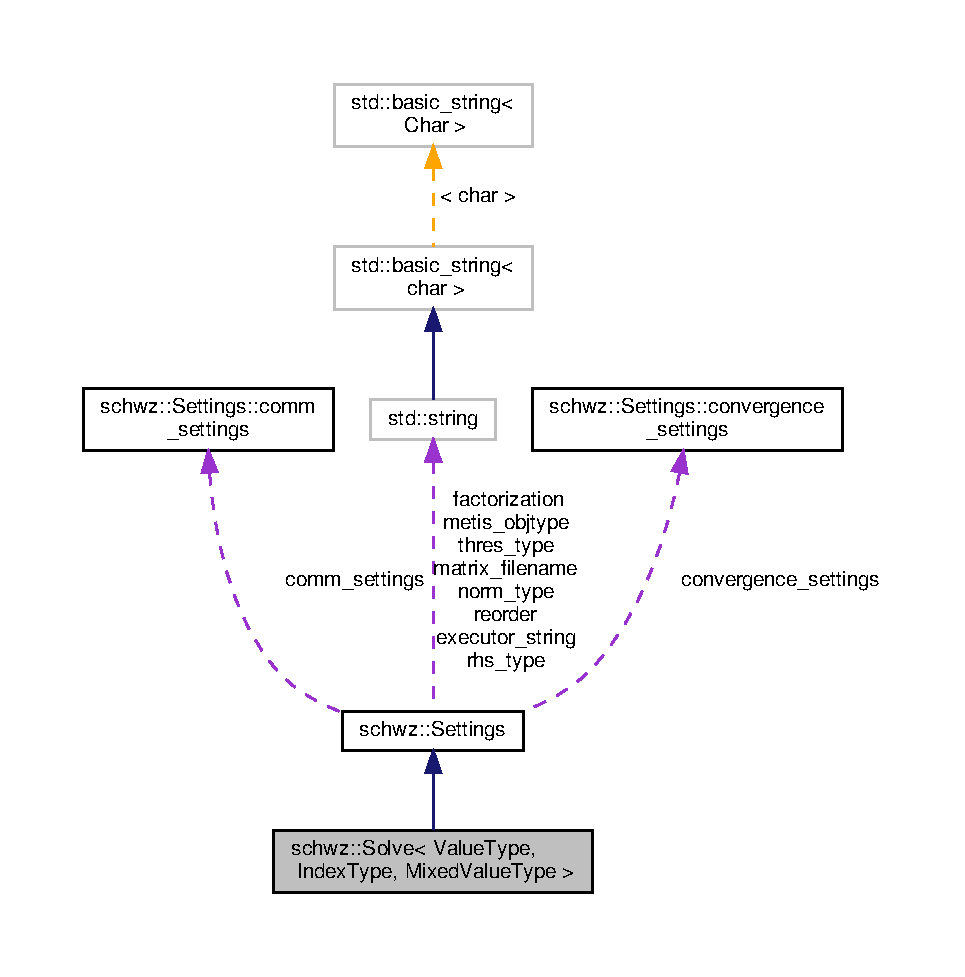
\includegraphics[width=350pt]{classschwz_1_1Solve__coll__graph}
\end{center}
\end{figure}
\subsection*{Public Member Functions}
\begin{DoxyCompactItemize}
\item 
\mbox{\Hypertarget{classschwz_1_1Solve_a24250987949518cc92649066d3ce147d}\label{classschwz_1_1Solve_a24250987949518cc92649066d3ce147d}} 
{\bfseries Solve} (const \hyperlink{structschwz_1_1Settings}{Settings} \&settings)
\end{DoxyCompactItemize}
\subsection*{Friends}
\begin{DoxyCompactItemize}
\item 
\mbox{\Hypertarget{classschwz_1_1Solve_a7044b349fe5363eeace2d1a56b38f650}\label{classschwz_1_1Solve_a7044b349fe5363eeace2d1a56b38f650}} 
class {\bfseries Initialize$<$ Value\+Type, Index\+Type $>$}
\end{DoxyCompactItemize}
\subsection*{Additional Inherited Members}


\subsection{Detailed Description}
\subsubsection*{template$<$typename Value\+Type = gko\+::default\+\_\+precision, typename Index\+Type = gko\+::int32$>$\newline
class schwz\+::\+Solve$<$ Value\+Type, Index\+Type $>$}

The Solver class the provides the solver and the convergence checking methods. 


\begin{DoxyTemplParams}{Template Parameters}
{\em Value\+Type} & The type of the floating point values. \\
\hline
{\em Index\+Type} & The type of the index type values.\\
\hline
\end{DoxyTemplParams}
\hyperlink{group__solve}{Solve} 

The documentation for this class was generated from the following files\+:\begin{DoxyCompactItemize}
\item 
solve.\+hpp (6e759ed)\item 
/home/runner/work/schwarz-\/lib/schwarz-\/lib/source/solve.\+cpp (6e759ed)\end{DoxyCompactItemize}

\hypertarget{classschwz_1_1SolverRAS}{}\section{schwz\+:\+:Solver\+R\+AS$<$ Value\+Type, Index\+Type $>$ Class Template Reference}
\label{classschwz_1_1SolverRAS}\index{schwz\+::\+Solver\+R\+A\+S$<$ Value\+Type, Index\+Type $>$@{schwz\+::\+Solver\+R\+A\+S$<$ Value\+Type, Index\+Type $>$}}


An implementation of the solver interface using the R\+AS solver.  




{\ttfamily \#include $<$restricted\+\_\+schwarz.\+hpp$>$}



Collaboration diagram for schwz\+:\+:Solver\+R\+AS$<$ Value\+Type, Index\+Type $>$\+:
\nopagebreak
\begin{figure}[H]
\begin{center}
\leavevmode
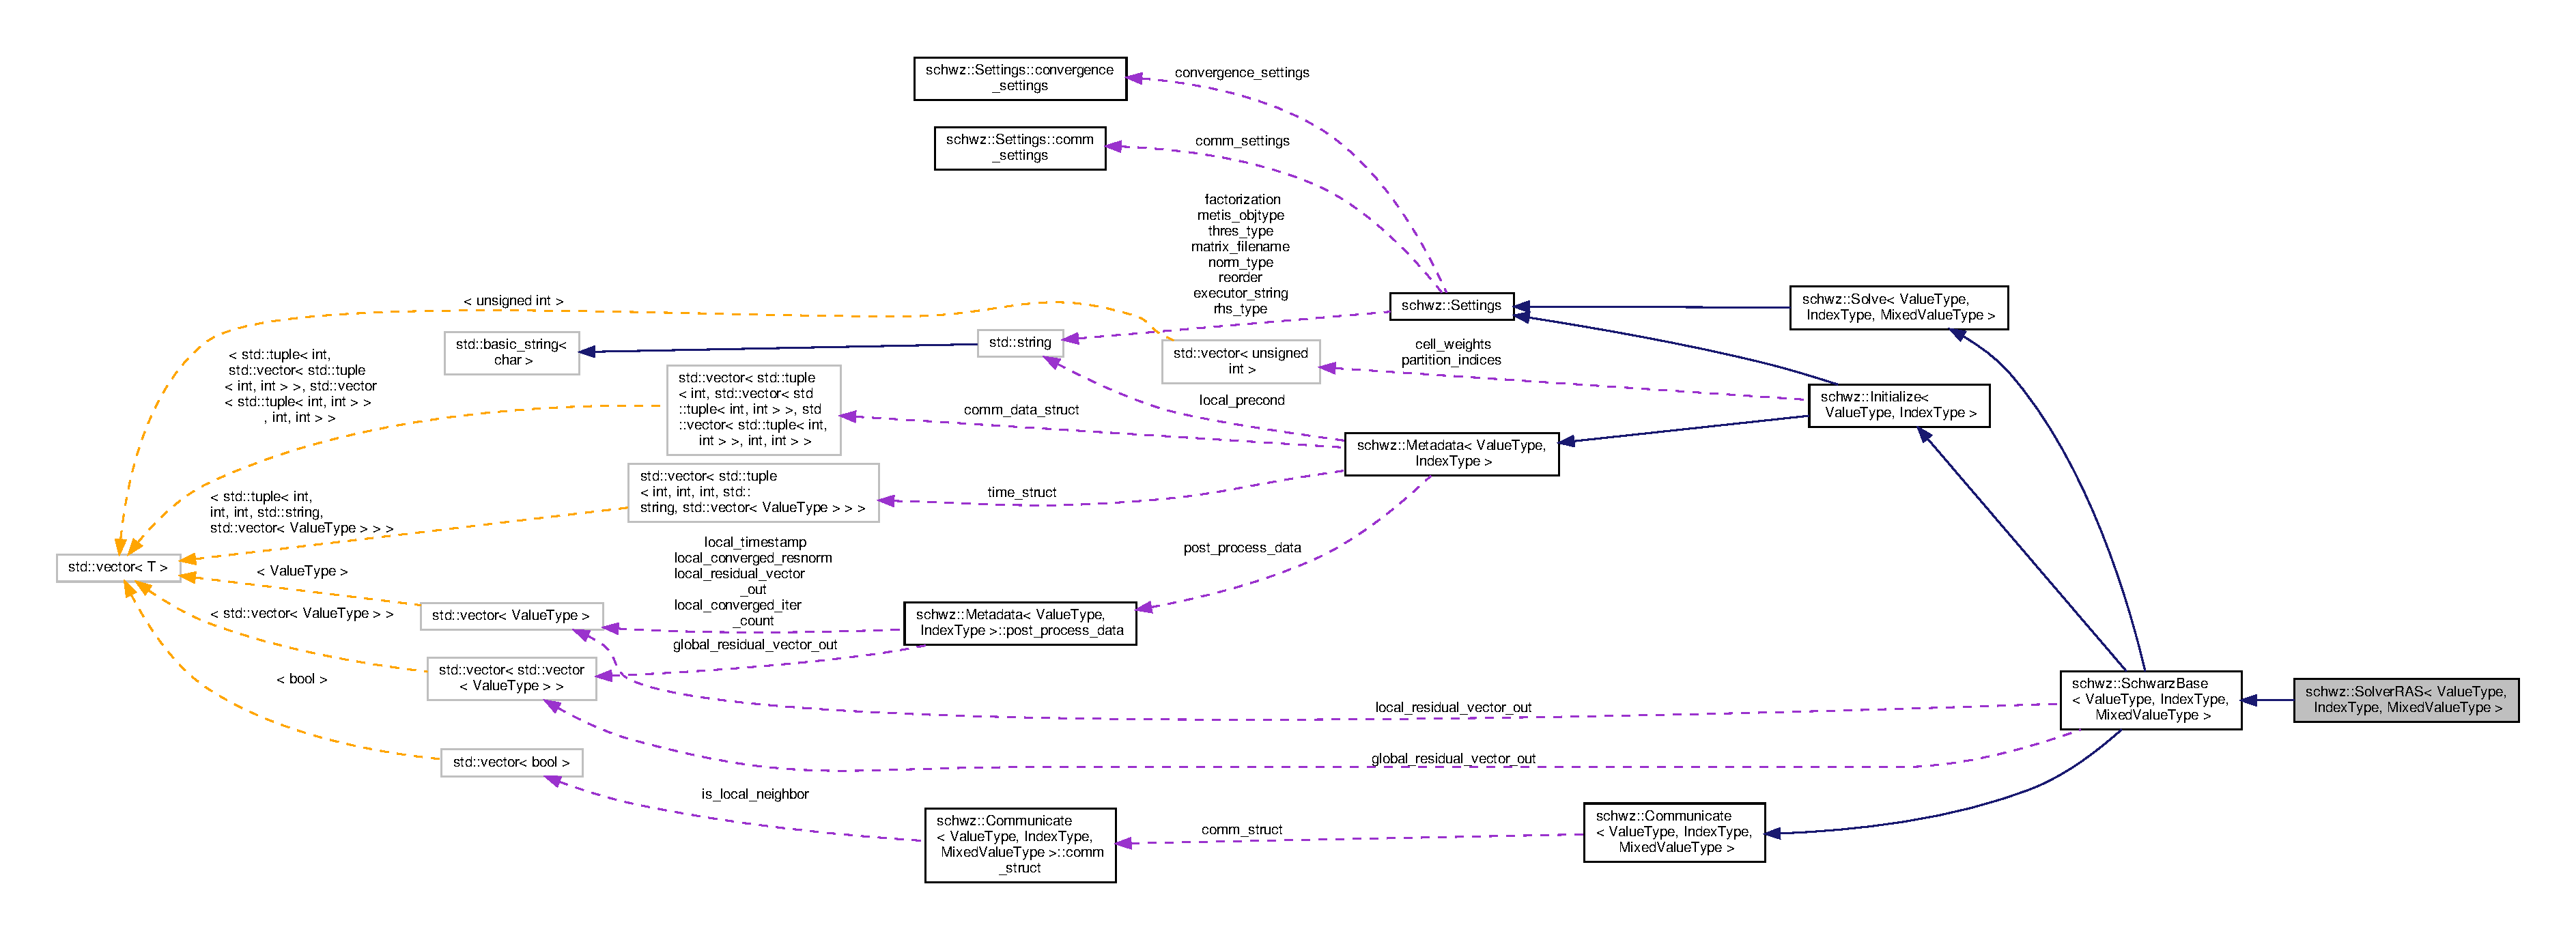
\includegraphics[width=350pt]{classschwz_1_1SolverRAS__coll__graph}
\end{center}
\end{figure}
\subsection*{Public Member Functions}
\begin{DoxyCompactItemize}
\item 
\hyperlink{classschwz_1_1SolverRAS_a3af020a3c088ad73024c00b2af4910f0}{Solver\+R\+AS} (\hyperlink{structschwz_1_1Settings}{Settings} \&settings, \hyperlink{structschwz_1_1Metadata}{Metadata}$<$ Value\+Type, Index\+Type $>$ \&metadata)
\begin{DoxyCompactList}\small\item\em The constructor that takes in the user settings and a metadata struct containing the solver metadata. \end{DoxyCompactList}\item 
void \hyperlink{classschwz_1_1SolverRAS_aebbdd245b7019af802606ad95a8e3a5a}{setup\+\_\+local\+\_\+matrices} (\hyperlink{structschwz_1_1Settings}{Settings} \&settings, \hyperlink{structschwz_1_1Metadata}{Metadata}$<$ Value\+Type, Index\+Type $>$ \&metadata, std\+::vector$<$ unsigned int $>$ \&\hyperlink{classschwz_1_1Initialize_a007426e21221298b6dca9b7c9fbd1c10}{partition\+\_\+indices}, std\+::shared\+\_\+ptr$<$ gko\+::matrix\+::\+Csr$<$ Value\+Type, Index\+Type $>$$>$ \&\hyperlink{classschwz_1_1SchwarzBase_a3539b68fb6ff07a8f58b1f990976dc90}{global\+\_\+matrix}, std\+::shared\+\_\+ptr$<$ gko\+::matrix\+::\+Csr$<$ Value\+Type, Index\+Type $>$$>$ \&\hyperlink{classschwz_1_1SchwarzBase_a64bdd55bbab23c6e21d0621cd84a299b}{local\+\_\+matrix}, std\+::shared\+\_\+ptr$<$ gko\+::matrix\+::\+Csr$<$ Value\+Type, Index\+Type $>$$>$ \&\hyperlink{classschwz_1_1SchwarzBase_a1e9742522b50a7bebe936b6540694f72}{interface\+\_\+matrix}) override
\begin{DoxyCompactList}\small\item\em Sets up the local and the interface matrices from the global matrix and the partition indices. \end{DoxyCompactList}\item 
\mbox{\Hypertarget{classschwz_1_1SolverRAS_a167b67ab0fb9d46244e9de563a682b43}\label{classschwz_1_1SolverRAS_a167b67ab0fb9d46244e9de563a682b43}} 
void \hyperlink{classschwz_1_1SolverRAS_a167b67ab0fb9d46244e9de563a682b43}{setup\+\_\+comm\+\_\+buffers} () override
\begin{DoxyCompactList}\small\item\em Sets up the communication buffers needed for the boundary exchange. \end{DoxyCompactList}\item 
void \hyperlink{classschwz_1_1SolverRAS_a8cd640aa073c0890d6121dc3afb3eaac}{setup\+\_\+windows} (const \hyperlink{structschwz_1_1Settings}{Settings} \&settings, const \hyperlink{structschwz_1_1Metadata}{Metadata}$<$ Value\+Type, Index\+Type $>$ \&metadata, std\+::shared\+\_\+ptr$<$ gko\+::matrix\+::\+Dense$<$ Value\+Type $>$$>$ \&main\+\_\+buffer) override
\begin{DoxyCompactList}\small\item\em Sets up the windows needed for the asynchronous communication. \end{DoxyCompactList}\item 
void \hyperlink{classschwz_1_1SolverRAS_a30a7b9e8ae4852fce06e407ea620ddbb}{exchange\+\_\+boundary} (const \hyperlink{structschwz_1_1Settings}{Settings} \&settings, const \hyperlink{structschwz_1_1Metadata}{Metadata}$<$ Value\+Type, Index\+Type $>$ \&metadata, std\+::shared\+\_\+ptr$<$ gko\+::matrix\+::\+Dense$<$ Value\+Type $>$$>$ \&\hyperlink{classschwz_1_1SchwarzBase_a8e6f088b8a7112af2ce27285d8d91bcc}{global\+\_\+solution}) override
\begin{DoxyCompactList}\small\item\em Exchanges the elements of the solution vector. \end{DoxyCompactList}\item 
void \hyperlink{classschwz_1_1SolverRAS_a974f6e6be558338a37bdc65f34afdb26}{update\+\_\+boundary} (const \hyperlink{structschwz_1_1Settings}{Settings} \&settings, const \hyperlink{structschwz_1_1Metadata}{Metadata}$<$ Value\+Type, Index\+Type $>$ \&metadata, std\+::shared\+\_\+ptr$<$ gko\+::matrix\+::\+Dense$<$ Value\+Type $>$$>$ \&\hyperlink{classschwz_1_1SchwarzBase_a29ef68da307b6de9b8ae878df8fb19d4}{local\+\_\+solution}, const std\+::shared\+\_\+ptr$<$ gko\+::matrix\+::\+Dense$<$ Value\+Type $>$$>$ \&\hyperlink{classschwz_1_1SchwarzBase_ac28b3e811e6016f31836fe366ff56eb7}{local\+\_\+rhs}, const std\+::shared\+\_\+ptr$<$ gko\+::matrix\+::\+Dense$<$ Value\+Type $>$$>$ \&\hyperlink{classschwz_1_1SchwarzBase_a8e6f088b8a7112af2ce27285d8d91bcc}{global\+\_\+solution}, const std\+::shared\+\_\+ptr$<$ gko\+::matrix\+::\+Csr$<$ Value\+Type, Index\+Type $>$$>$ \&\hyperlink{classschwz_1_1SchwarzBase_a1e9742522b50a7bebe936b6540694f72}{interface\+\_\+matrix}) override
\begin{DoxyCompactList}\small\item\em Update the values into local vector from obtained from the neighboring sub-\/domains using the interface matrix. \end{DoxyCompactList}\end{DoxyCompactItemize}
\subsection*{Additional Inherited Members}


\subsection{Detailed Description}
\subsubsection*{template$<$typename Value\+Type = gko\+::default\+\_\+precision, typename Index\+Type = gko\+::int32$>$\newline
class schwz\+::\+Solver\+R\+A\+S$<$ Value\+Type, Index\+Type $>$}

An implementation of the solver interface using the R\+AS solver. 


\begin{DoxyTemplParams}{Template Parameters}
{\em Value\+Type} & The type of the floating point values. \\
\hline
{\em Index\+Type} & The type of the index type values. \\
\hline
\end{DoxyTemplParams}


\subsection{Constructor \& Destructor Documentation}
\mbox{\Hypertarget{classschwz_1_1SolverRAS_a3af020a3c088ad73024c00b2af4910f0}\label{classschwz_1_1SolverRAS_a3af020a3c088ad73024c00b2af4910f0}} 
\index{schwz\+::\+Solver\+R\+AS@{schwz\+::\+Solver\+R\+AS}!Solver\+R\+AS@{Solver\+R\+AS}}
\index{Solver\+R\+AS@{Solver\+R\+AS}!schwz\+::\+Solver\+R\+AS@{schwz\+::\+Solver\+R\+AS}}
\subsubsection{\texorpdfstring{Solver\+R\+A\+S()}{SolverRAS()}}
{\footnotesize\ttfamily template$<$typename Value\+Type , typename Index\+Type $>$ \\
\hyperlink{classschwz_1_1SolverRAS}{schwz\+::\+Solver\+R\+AS}$<$ Value\+Type, Index\+Type $>$\+::\hyperlink{classschwz_1_1SolverRAS}{Solver\+R\+AS} (\begin{DoxyParamCaption}\item[{\hyperlink{structschwz_1_1Settings}{Settings} \&}]{settings,  }\item[{\hyperlink{structschwz_1_1Metadata}{Metadata}$<$ Value\+Type, Index\+Type $>$ \&}]{metadata }\end{DoxyParamCaption})}



The constructor that takes in the user settings and a metadata struct containing the solver metadata. 


\begin{DoxyParams}{Parameters}
{\em settings} & The settings struct. \\
\hline
{\em metadata} & The metadata struct. \\
\hline
{\em data} & The additional data struct. \\
\hline
\end{DoxyParams}


\subsection{Member Function Documentation}
\mbox{\Hypertarget{classschwz_1_1SolverRAS_a30a7b9e8ae4852fce06e407ea620ddbb}\label{classschwz_1_1SolverRAS_a30a7b9e8ae4852fce06e407ea620ddbb}} 
\index{schwz\+::\+Solver\+R\+AS@{schwz\+::\+Solver\+R\+AS}!exchange\+\_\+boundary@{exchange\+\_\+boundary}}
\index{exchange\+\_\+boundary@{exchange\+\_\+boundary}!schwz\+::\+Solver\+R\+AS@{schwz\+::\+Solver\+R\+AS}}
\subsubsection{\texorpdfstring{exchange\+\_\+boundary()}{exchange\_boundary()}}
{\footnotesize\ttfamily template$<$typename Value\+Type , typename Index\+Type $>$ \\
void \hyperlink{classschwz_1_1SolverRAS}{schwz\+::\+Solver\+R\+AS}$<$ Value\+Type, Index\+Type $>$\+::exchange\+\_\+boundary (\begin{DoxyParamCaption}\item[{const \hyperlink{structschwz_1_1Settings}{Settings} \&}]{settings,  }\item[{const \hyperlink{structschwz_1_1Metadata}{Metadata}$<$ Value\+Type, Index\+Type $>$ \&}]{metadata,  }\item[{std\+::shared\+\_\+ptr$<$ gko\+::matrix\+::\+Dense$<$ Value\+Type $>$$>$ \&}]{global\+\_\+solution }\end{DoxyParamCaption})\hspace{0.3cm}{\ttfamily [override]}, {\ttfamily [virtual]}}



Exchanges the elements of the solution vector. 


\begin{DoxyParams}{Parameters}
{\em settings} & The settings struct. \\
\hline
{\em metadata} & The metadata struct. \\
\hline
{\em global\+\_\+solution} & The solution vector being exchanged between the subdomains. \\
\hline
\end{DoxyParams}


Implements \hyperlink{classschwz_1_1Communicate_a9f305bc37b86b1cf9369acdf6fe32f7d}{schwz\+::\+Communicate$<$ Value\+Type, Index\+Type $>$}.



References schwz\+::\+Settings\+::comm\+\_\+settings\+::enable\+\_\+onesided, and schwz\+::\+Schwarz\+Base$<$ Value\+Type, Index\+Type $>$\+::global\+\_\+solution.

\mbox{\Hypertarget{classschwz_1_1SolverRAS_aebbdd245b7019af802606ad95a8e3a5a}\label{classschwz_1_1SolverRAS_aebbdd245b7019af802606ad95a8e3a5a}} 
\index{schwz\+::\+Solver\+R\+AS@{schwz\+::\+Solver\+R\+AS}!setup\+\_\+local\+\_\+matrices@{setup\+\_\+local\+\_\+matrices}}
\index{setup\+\_\+local\+\_\+matrices@{setup\+\_\+local\+\_\+matrices}!schwz\+::\+Solver\+R\+AS@{schwz\+::\+Solver\+R\+AS}}
\subsubsection{\texorpdfstring{setup\+\_\+local\+\_\+matrices()}{setup\_local\_matrices()}}
{\footnotesize\ttfamily template$<$typename Value\+Type , typename Index\+Type $>$ \\
void \hyperlink{classschwz_1_1SolverRAS}{schwz\+::\+Solver\+R\+AS}$<$ Value\+Type, Index\+Type $>$\+::setup\+\_\+local\+\_\+matrices (\begin{DoxyParamCaption}\item[{\hyperlink{structschwz_1_1Settings}{Settings} \&}]{settings,  }\item[{\hyperlink{structschwz_1_1Metadata}{Metadata}$<$ Value\+Type, Index\+Type $>$ \&}]{metadata,  }\item[{std\+::vector$<$ unsigned int $>$ \&}]{partition\+\_\+indices,  }\item[{std\+::shared\+\_\+ptr$<$ gko\+::matrix\+::\+Csr$<$ Value\+Type, Index\+Type $>$$>$ \&}]{global\+\_\+matrix,  }\item[{std\+::shared\+\_\+ptr$<$ gko\+::matrix\+::\+Csr$<$ Value\+Type, Index\+Type $>$$>$ \&}]{local\+\_\+matrix,  }\item[{std\+::shared\+\_\+ptr$<$ gko\+::matrix\+::\+Csr$<$ Value\+Type, Index\+Type $>$$>$ \&}]{interface\+\_\+matrix }\end{DoxyParamCaption})\hspace{0.3cm}{\ttfamily [override]}, {\ttfamily [virtual]}}



Sets up the local and the interface matrices from the global matrix and the partition indices. 


\begin{DoxyParams}{Parameters}
{\em settings} & The settings struct. \\
\hline
{\em metadata} & The metadata struct. \\
\hline
{\em partition\+\_\+indices} & The array containing the partition indices. \\
\hline
{\em global\+\_\+matrix} & The global system matrix. \\
\hline
{\em local\+\_\+matrix} & The local system matrix. \\
\hline
{\em interface\+\_\+matrix} & The interface matrix containing the interface and the overlap data mainly used for exchanging values between different sub-\/domains. \\
\hline
{\em local\+\_\+perm} & The local permutation, obtained through R\+CM or M\+E\+T\+IS. \\
\hline
\end{DoxyParams}


Implements \hyperlink{classschwz_1_1Initialize_ad24764a4ded54c2af6a5111ba8c8228f}{schwz\+::\+Initialize$<$ Value\+Type, Index\+Type $>$}.



References schwz\+::\+Metadata$<$ Value\+Type, Index\+Type $>$\+::comm\+\_\+size, schwz\+::\+Settings\+::executor, schwz\+::\+Metadata$<$ Value\+Type, Index\+Type $>$\+::first\+\_\+row, schwz\+::\+Schwarz\+Base$<$ Value\+Type, Index\+Type $>$\+::global\+\_\+matrix, schwz\+::\+Metadata$<$ Value\+Type, Index\+Type $>$\+::global\+\_\+size, schwz\+::\+Metadata$<$ Value\+Type, Index\+Type $>$\+::global\+\_\+to\+\_\+local, schwz\+::\+Metadata$<$ Value\+Type, Index\+Type $>$\+::i\+\_\+permutation, schwz\+::\+Schwarz\+Base$<$ Value\+Type, Index\+Type $>$\+::interface\+\_\+matrix, schwz\+::\+Schwarz\+Base$<$ Value\+Type, Index\+Type $>$\+::local\+\_\+matrix, schwz\+::\+Metadata$<$ Value\+Type, Index\+Type $>$\+::local\+\_\+size, schwz\+::\+Metadata$<$ Value\+Type, Index\+Type $>$\+::local\+\_\+size\+\_\+o, schwz\+::\+Metadata$<$ Value\+Type, Index\+Type $>$\+::local\+\_\+size\+\_\+x, schwz\+::\+Metadata$<$ Value\+Type, Index\+Type $>$\+::local\+\_\+to\+\_\+global, schwz\+::\+Metadata$<$ Value\+Type, Index\+Type $>$\+::my\+\_\+rank, schwz\+::\+Metadata$<$ Value\+Type, Index\+Type $>$\+::num\+\_\+subdomains, schwz\+::\+Settings\+::overlap, schwz\+::\+Metadata$<$ Value\+Type, Index\+Type $>$\+::overlap\+\_\+row, schwz\+::\+Metadata$<$ Value\+Type, Index\+Type $>$\+::overlap\+\_\+size, and schwz\+::\+Metadata$<$ Value\+Type, Index\+Type $>$\+::permutation.

\mbox{\Hypertarget{classschwz_1_1SolverRAS_a8cd640aa073c0890d6121dc3afb3eaac}\label{classschwz_1_1SolverRAS_a8cd640aa073c0890d6121dc3afb3eaac}} 
\index{schwz\+::\+Solver\+R\+AS@{schwz\+::\+Solver\+R\+AS}!setup\+\_\+windows@{setup\+\_\+windows}}
\index{setup\+\_\+windows@{setup\+\_\+windows}!schwz\+::\+Solver\+R\+AS@{schwz\+::\+Solver\+R\+AS}}
\subsubsection{\texorpdfstring{setup\+\_\+windows()}{setup\_windows()}}
{\footnotesize\ttfamily template$<$typename Value\+Type , typename Index\+Type $>$ \\
void \hyperlink{classschwz_1_1SolverRAS}{schwz\+::\+Solver\+R\+AS}$<$ Value\+Type, Index\+Type $>$\+::setup\+\_\+windows (\begin{DoxyParamCaption}\item[{const \hyperlink{structschwz_1_1Settings}{Settings} \&}]{settings,  }\item[{const \hyperlink{structschwz_1_1Metadata}{Metadata}$<$ Value\+Type, Index\+Type $>$ \&}]{metadata,  }\item[{std\+::shared\+\_\+ptr$<$ gko\+::matrix\+::\+Dense$<$ Value\+Type $>$$>$ \&}]{main\+\_\+buffer }\end{DoxyParamCaption})\hspace{0.3cm}{\ttfamily [override]}, {\ttfamily [virtual]}}



Sets up the windows needed for the asynchronous communication. 


\begin{DoxyParams}{Parameters}
{\em settings} & The settings struct. \\
\hline
{\em metadata} & The metadata struct. \\
\hline
{\em main\+\_\+buffer} & The main buffer being exchanged between the subdomains. \\
\hline
\end{DoxyParams}


Implements \hyperlink{classschwz_1_1Communicate_ab41e8e19e90ce2d53234cbec2cdb3b38}{schwz\+::\+Communicate$<$ Value\+Type, Index\+Type $>$}.



References schwz\+::\+Settings\+::comm\+\_\+settings\+::enable\+\_\+get, schwz\+::\+Settings\+::comm\+\_\+settings\+::enable\+\_\+lock\+\_\+all, schwz\+::\+Settings\+::comm\+\_\+settings\+::enable\+\_\+one\+\_\+by\+\_\+one, schwz\+::\+Settings\+::comm\+\_\+settings\+::enable\+\_\+onesided, schwz\+::\+Settings\+::comm\+\_\+settings\+::enable\+\_\+overlap, schwz\+::\+Settings\+::comm\+\_\+settings\+::enable\+\_\+put, schwz\+::\+Settings\+::executor, schwz\+::\+Communicate$<$ Value\+Type, Index\+Type $>$\+::comm\+\_\+struct\+::get\+\_\+displacements, schwz\+::\+Communicate$<$ Value\+Type, Index\+Type $>$\+::comm\+\_\+struct\+::get\+\_\+request, schwz\+::\+Communicate$<$ Value\+Type, Index\+Type $>$\+::comm\+\_\+struct\+::global\+\_\+get, schwz\+::\+Communicate$<$ Value\+Type, Index\+Type $>$\+::comm\+\_\+struct\+::global\+\_\+put, schwz\+::\+Schwarz\+Base$<$ Value\+Type, Index\+Type $>$\+::global\+\_\+solution, schwz\+::\+Communicate$<$ Value\+Type, Index\+Type $>$\+::comm\+\_\+struct\+::is\+\_\+local\+\_\+neighbor, schwz\+::\+Metadata$<$ Value\+Type, Index\+Type $>$\+::iter\+\_\+count, schwz\+::\+Communicate$<$ Value\+Type, Index\+Type $>$\+::comm\+\_\+struct\+::local\+\_\+get, schwz\+::\+Communicate$<$ Value\+Type, Index\+Type $>$\+::comm\+\_\+struct\+::local\+\_\+neighbors\+\_\+in, schwz\+::\+Communicate$<$ Value\+Type, Index\+Type $>$\+::comm\+\_\+struct\+::local\+\_\+neighbors\+\_\+out, schwz\+::\+Communicate$<$ Value\+Type, Index\+Type $>$\+::comm\+\_\+struct\+::local\+\_\+num\+\_\+neighbors\+\_\+in, schwz\+::\+Communicate$<$ Value\+Type, Index\+Type $>$\+::comm\+\_\+struct\+::local\+\_\+num\+\_\+neighbors\+\_\+out, schwz\+::\+Communicate$<$ Value\+Type, Index\+Type $>$\+::comm\+\_\+struct\+::local\+\_\+put, schwz\+::\+Metadata$<$ Value\+Type, Index\+Type $>$\+::local\+\_\+size\+\_\+o, schwz\+::\+Schwarz\+Base$<$ Value\+Type, Index\+Type $>$\+::local\+\_\+solution, schwz\+::\+Communicate$<$ Value\+Type, Index\+Type $>$\+::comm\+\_\+struct\+::neighbors\+\_\+in, schwz\+::\+Communicate$<$ Value\+Type, Index\+Type $>$\+::comm\+\_\+struct\+::neighbors\+\_\+out, schwz\+::\+Communicate$<$ Value\+Type, Index\+Type $>$\+::comm\+\_\+struct\+::num\+\_\+neighbors\+\_\+in, schwz\+::\+Communicate$<$ Value\+Type, Index\+Type $>$\+::comm\+\_\+struct\+::num\+\_\+neighbors\+\_\+out, schwz\+::\+Metadata$<$ Value\+Type, Index\+Type $>$\+::num\+\_\+subdomains, schwz\+::\+Communicate$<$ Value\+Type, Index\+Type $>$\+::comm\+\_\+struct\+::put\+\_\+displacements, schwz\+::\+Communicate$<$ Value\+Type, Index\+Type $>$\+::comm\+\_\+struct\+::put\+\_\+request, schwz\+::\+Communicate$<$ Value\+Type, Index\+Type $>$\+::comm\+\_\+struct\+::recv\+\_\+buffer, schwz\+::\+Communicate$<$ Value\+Type, Index\+Type $>$\+::comm\+\_\+struct\+::remote\+\_\+get, schwz\+::\+Communicate$<$ Value\+Type, Index\+Type $>$\+::comm\+\_\+struct\+::remote\+\_\+put, schwz\+::\+Communicate$<$ Value\+Type, Index\+Type $>$\+::comm\+\_\+struct\+::send\+\_\+buffer, schwz\+::\+Communicate$<$ Value\+Type, Index\+Type $>$\+::comm\+\_\+struct\+::window\+\_\+recv\+\_\+buffer, schwz\+::\+Communicate$<$ Value\+Type, Index\+Type $>$\+::comm\+\_\+struct\+::window\+\_\+send\+\_\+buffer, and schwz\+::\+Communicate$<$ Value\+Type, Index\+Type $>$\+::comm\+\_\+struct\+::window\+\_\+x.

\mbox{\Hypertarget{classschwz_1_1SolverRAS_a974f6e6be558338a37bdc65f34afdb26}\label{classschwz_1_1SolverRAS_a974f6e6be558338a37bdc65f34afdb26}} 
\index{schwz\+::\+Solver\+R\+AS@{schwz\+::\+Solver\+R\+AS}!update\+\_\+boundary@{update\+\_\+boundary}}
\index{update\+\_\+boundary@{update\+\_\+boundary}!schwz\+::\+Solver\+R\+AS@{schwz\+::\+Solver\+R\+AS}}
\subsubsection{\texorpdfstring{update\+\_\+boundary()}{update\_boundary()}}
{\footnotesize\ttfamily template$<$typename Value\+Type , typename Index\+Type $>$ \\
void \hyperlink{classschwz_1_1SolverRAS}{schwz\+::\+Solver\+R\+AS}$<$ Value\+Type, Index\+Type $>$\+::update\+\_\+boundary (\begin{DoxyParamCaption}\item[{const \hyperlink{structschwz_1_1Settings}{Settings} \&}]{settings,  }\item[{const \hyperlink{structschwz_1_1Metadata}{Metadata}$<$ Value\+Type, Index\+Type $>$ \&}]{metadata,  }\item[{std\+::shared\+\_\+ptr$<$ gko\+::matrix\+::\+Dense$<$ Value\+Type $>$$>$ \&}]{local\+\_\+solution,  }\item[{const std\+::shared\+\_\+ptr$<$ gko\+::matrix\+::\+Dense$<$ Value\+Type $>$$>$ \&}]{local\+\_\+rhs,  }\item[{const std\+::shared\+\_\+ptr$<$ gko\+::matrix\+::\+Dense$<$ Value\+Type $>$$>$ \&}]{global\+\_\+solution,  }\item[{const std\+::shared\+\_\+ptr$<$ gko\+::matrix\+::\+Csr$<$ Value\+Type, Index\+Type $>$$>$ \&}]{interface\+\_\+matrix }\end{DoxyParamCaption})\hspace{0.3cm}{\ttfamily [override]}, {\ttfamily [virtual]}}



Update the values into local vector from obtained from the neighboring sub-\/domains using the interface matrix. 


\begin{DoxyParams}{Parameters}
{\em settings} & The settings struct. \\
\hline
{\em metadata} & The metadata struct. \\
\hline
{\em local\+\_\+solution} & The local solution vector in the subdomain. \\
\hline
{\em local\+\_\+rhs} & The local right hand side vector in the subdomain. \\
\hline
{\em global\+\_\+solution} & The workspace solution vector. \\
\hline
{\em global\+\_\+old\+\_\+solution} & The global solution vector of the previous iteration. \\
\hline
{\em interface\+\_\+matrix} & The interface matrix containing the interface and the overlap data mainly used for exchanging values between different sub-\/domains. \\
\hline
\end{DoxyParams}


Implements \hyperlink{classschwz_1_1Communicate_aa1332376dfc67f5384527be90df7cbea}{schwz\+::\+Communicate$<$ Value\+Type, Index\+Type $>$}.



References schwz\+::\+Settings\+::executor, schwz\+::\+Schwarz\+Base$<$ Value\+Type, Index\+Type $>$\+::global\+\_\+solution, schwz\+::\+Schwarz\+Base$<$ Value\+Type, Index\+Type $>$\+::interface\+\_\+matrix, schwz\+::\+Schwarz\+Base$<$ Value\+Type, Index\+Type $>$\+::local\+\_\+rhs, schwz\+::\+Metadata$<$ Value\+Type, Index\+Type $>$\+::local\+\_\+size\+\_\+x, schwz\+::\+Schwarz\+Base$<$ Value\+Type, Index\+Type $>$\+::local\+\_\+solution, schwz\+::\+Metadata$<$ Value\+Type, Index\+Type $>$\+::num\+\_\+subdomains, and schwz\+::\+Settings\+::overlap.



The documentation for this class was generated from the following files\+:\begin{DoxyCompactItemize}
\item 
restricted\+\_\+schwarz.\+hpp (6e759ed)\item 
/home/runner/work/schwarz-\/lib/schwarz-\/lib/source/restricted\+\_\+schwarz.\+cpp (6e759ed)\end{DoxyCompactItemize}

\hypertarget{classUmfpackError}{}\section{Umfpack\+Error Class Reference}
\label{classUmfpackError}\index{Umfpack\+Error@{Umfpack\+Error}}


\hyperlink{classUmfpackError}{Umfpack\+Error} is thrown when a M\+E\+T\+IS routine throws a non-\/zero error code.  




{\ttfamily \#include $<$exception.\+hpp$>$}



Collaboration diagram for Umfpack\+Error\+:
\nopagebreak
\begin{figure}[H]
\begin{center}
\leavevmode
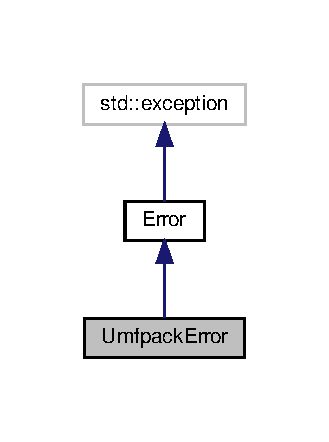
\includegraphics[width=158pt]{classUmfpackError__coll__graph}
\end{center}
\end{figure}
\subsection*{Public Member Functions}
\begin{DoxyCompactItemize}
\item 
\hyperlink{classUmfpackError_a3df702dc59370f9ff8f097f8657d3fff}{Umfpack\+Error} (const std\+::string \&file, int line, const std\+::string \&func, int error\+\_\+code)
\begin{DoxyCompactList}\small\item\em Initializes a M\+E\+T\+IS error. \end{DoxyCompactList}\end{DoxyCompactItemize}


\subsection{Detailed Description}
\hyperlink{classUmfpackError}{Umfpack\+Error} is thrown when a M\+E\+T\+IS routine throws a non-\/zero error code. 

\subsection{Constructor \& Destructor Documentation}
\mbox{\Hypertarget{classUmfpackError_a3df702dc59370f9ff8f097f8657d3fff}\label{classUmfpackError_a3df702dc59370f9ff8f097f8657d3fff}} 
\index{Umfpack\+Error@{Umfpack\+Error}!Umfpack\+Error@{Umfpack\+Error}}
\index{Umfpack\+Error@{Umfpack\+Error}!Umfpack\+Error@{Umfpack\+Error}}
\subsubsection{\texorpdfstring{Umfpack\+Error()}{UmfpackError()}}
{\footnotesize\ttfamily Umfpack\+Error\+::\+Umfpack\+Error (\begin{DoxyParamCaption}\item[{const std\+::string \&}]{file,  }\item[{int}]{line,  }\item[{const std\+::string \&}]{func,  }\item[{int}]{error\+\_\+code }\end{DoxyParamCaption})\hspace{0.3cm}{\ttfamily [inline]}}



Initializes a M\+E\+T\+IS error. 


\begin{DoxyParams}{Parameters}
{\em file} & The name of the offending source file \\
\hline
{\em line} & The source code line number where the error occurred \\
\hline
{\em func} & The name of the M\+E\+T\+IS routine that failed \\
\hline
{\em error\+\_\+code} & The resulting M\+E\+T\+IS error code \\
\hline
\end{DoxyParams}


The documentation for this class was generated from the following files\+:\begin{DoxyCompactItemize}
\item 
exception.\+hpp (04a42d4)\item 
/home/runner/work/schwarz-\/lib/schwarz-\/lib/source/exception.\+cpp (04a42d4)\end{DoxyCompactItemize}

\hypertarget{structschwz_1_1Utils}{}\section{schwz\+:\+:Utils$<$ Value\+Type, Index\+Type $>$ Struct Template Reference}
\label{structschwz_1_1Utils}\index{schwz\+::\+Utils$<$ Value\+Type, Index\+Type $>$@{schwz\+::\+Utils$<$ Value\+Type, Index\+Type $>$}}


The utilities class which provides some checks and basic utilities.  




{\ttfamily \#include $<$utils.\+hpp$>$}

\subsection*{Static Public Member Functions}
\begin{DoxyCompactItemize}
\item 
\mbox{\Hypertarget{structschwz_1_1Utils_a6f65fc83d6270453712a2600bab557ce}\label{structschwz_1_1Utils_a6f65fc83d6270453712a2600bab557ce}} 
static int {\bfseries get\+\_\+local\+\_\+rank} (M\+P\+I\+\_\+\+Comm mpi\+\_\+communicator)
\item 
\mbox{\Hypertarget{structschwz_1_1Utils_a33d613297cb2b53634c1ed2b44fe595c}\label{structschwz_1_1Utils_a33d613297cb2b53634c1ed2b44fe595c}} 
static int {\bfseries get\+\_\+local\+\_\+num\+\_\+procs} (M\+P\+I\+\_\+\+Comm mpi\+\_\+communicator)
\item 
\mbox{\Hypertarget{structschwz_1_1Utils_a18df4f61989071e018f64ac7d7a1d6f1}\label{structschwz_1_1Utils_a18df4f61989071e018f64ac7d7a1d6f1}} 
static bool {\bfseries check\+\_\+subd\+\_\+locality} (M\+P\+I\+\_\+\+Comm mpi\+\_\+communicator, int neighbor\+\_\+rank, int my\+\_\+rank)
\item 
\mbox{\Hypertarget{structschwz_1_1Utils_a6f0494e5c7d6be0585e26efd1d1fa64c}\label{structschwz_1_1Utils_a6f0494e5c7d6be0585e26efd1d1fa64c}} 
static void {\bfseries print\+\_\+matrix} (const gko\+::matrix\+::\+Csr$<$ Value\+Type, Index\+Type $>$ $\ast$matrix, int rank, std\+::string name)
\item 
\mbox{\Hypertarget{structschwz_1_1Utils_a1abe3d1bde2091a0361f8beadb925f70}\label{structschwz_1_1Utils_a1abe3d1bde2091a0361f8beadb925f70}} 
static void {\bfseries print\+\_\+vector} (const gko\+::matrix\+::\+Dense$<$ Value\+Type $>$ $\ast$vector, int rank, std\+::string name)
\item 
\mbox{\Hypertarget{structschwz_1_1Utils_a391ddf4f24fb8d7c7ffacf8f046f94b5}\label{structschwz_1_1Utils_a391ddf4f24fb8d7c7ffacf8f046f94b5}} 
static int {\bfseries find\+\_\+duplicates} (Index\+Type val, std\+::size\+\_\+t index, const Index\+Type $\ast$data, std\+::size\+\_\+t length)
\item 
\mbox{\Hypertarget{structschwz_1_1Utils_a324726628a2cc9e0021069f5a060a140}\label{structschwz_1_1Utils_a324726628a2cc9e0021069f5a060a140}} 
static bool {\bfseries assert\+\_\+correct\+\_\+permutation} (const gko\+::matrix\+::\+Permutation$<$ Index\+Type $>$ $\ast$input\+\_\+perm)
\item 
\mbox{\Hypertarget{structschwz_1_1Utils_a6a86d7ed4bb4e8256378d0f5c31a20df}\label{structschwz_1_1Utils_a6a86d7ed4bb4e8256378d0f5c31a20df}} 
static bool {\bfseries assert\+\_\+correct\+\_\+cuda\+\_\+devices} (int num\+\_\+devices, int my\+\_\+rank)
\end{DoxyCompactItemize}


\subsection{Detailed Description}
\subsubsection*{template$<$typename Value\+Type = gko\+::default\+\_\+precision, typename Index\+Type = gko\+::int32$>$\newline
struct schwz\+::\+Utils$<$ Value\+Type, Index\+Type $>$}

The utilities class which provides some checks and basic utilities. 


\begin{DoxyTemplParams}{Template Parameters}
{\em Value\+Type} & The type of the floating point values. \\
\hline
{\em Index\+Type} & The type of the index type values.\\
\hline
\end{DoxyTemplParams}
\hyperlink{group__utils}{Utils} 

The documentation for this struct was generated from the following files\+:\begin{DoxyCompactItemize}
\item 
utils.\+hpp (f9e9a80)\item 
/home/runner/work/schwarz-\/lib/schwarz-\/lib/source/utils.\+cpp (f9e9a80)\end{DoxyCompactItemize}

%--- End generated contents ---

% Index
\backmatter
\newpage
\phantomsection
\clearemptydoublepage
\addcontentsline{toc}{chapter}{Index}
\printindex

\end{document}
